\documentclass[a4paper, 11pt]{scrbook}

\usepackage{style}
\usepackage{fullpage}

% Flag per escludere le immagini
\newif\iffigureon
\figureonfalse

% THEOREM ENVIORMMENT e.g. \newtheorem{comando}{nome}[numerazione]
\theoremstyle{definition}
\newtheorem{definition}{Definizione}[chapter]
\newtheorem{example}[definition]{Esempio}
\newtheorem{exercise}[definition]{Esercizio}

\theoremstyle{remark}
\newtheorem{oss}[definition]{Osservazione}

\theoremstyle{plain}
\newtheorem{thm}[definition]{Teorema}
\newtheorem{proposition}[definition]{Proposizione}
\newtheorem{lemma}[definition]{Lemma}

\newenvironment{solution}{\renewcommand\qedsymbol{}\begin{proof}[Soluzione]}{\end{proof}}

\numberwithin{equation}{chapter}

% DOCUMENT
\title{Introduzione ai sistemi dinamici I}
\author{SciSNS-2017}

\begin{document}
\frontmatter
\maketitle
Quest'opera è stata rilasciata con licenza Creative Commons Attribuzione - Non commerciale - Condividi allo stesso modo 4.0 Internazionale. Per leggere una copia della licenza visita il sito web \url{http://creativecommons.org/licenses/by-nc-sa/4.0/}.
\iffigureon
\begin{center}
    \href{http://creativecommons.org/licenses/by-nc-sa/4.0/}{\includegraphics[scale = 0.8]{img/by-nc-sa}}
\end{center}
\fi

Il progetto è ospitato su GitHub, dove si può trovare la versione più recente, al link \url{https://github.com/SciSNS-2017/Sistemi-Dinamici}. Ogni suggerimento (errori, soluzioni di esercizi, contributi vari, ecc.) è sempre gradito e può essere segnalato creando una \emph{issue} su GitHub oppure contattando direttamente gli autori.

\tableofcontents

\mainmatter
\chapter{Lezioni}
\section{Lezione del 09/10/2018 [Marmi]}
\begin{definition}[gruppo]
	Un gruppo è una coppia $ \mathcal{G} \coloneqq (G, \star) $ dove $ G $ è un insieme e $ {\star \colon G \times G \to G} $ è un'operazione binaria che gode delle seguenti proprietà
	\begin{enumerate}[label=(\roman*)]
		\item \emph{associativa}: $ \forall g_1, g_2, g_3 \in G, \ g_1 \star (g_2 \star g_3) = (g_1 \star g_2) \star g_3 $;
		\item \emph{elemento neutro sinistro}: $  \exists e \in G : \forall g \in G, \ g \star e = g $;
		\item \emph{inverso sinistro}: $ \forall g \in G, \exists g^{-1} \in G : g \star g^{-1} = e $.
	\end{enumerate}
	A partire da queste si mostra facilmente che l'elemento neutro destro è anche elemento neutro sinistro, l'inverso destro è anche inverso sinistro, che l'elemento neutro e l'inverso sono unici. \\
	Se non ci sono ambiguità circa l'operazione definita su $ G $ indicheremo più semplicemente il gruppo $ \mathcal{G} $ facendo riferimento al solo insieme $ G $. 
\end{definition}

\begin{definition}[sistema dinamico] \label{def:sistema-dinamico}
	Un sistema dinamico è una terna $ (\mathcal{G}, \mathcal{X}, \Phi) $ dove $ {\mathcal{G} \coloneqq (G, \star)} $ è un (semi-)gruppo\footnote{Per \emph{semigruppo} si intende una coppia $ (G,\star) $ dove $ \star $ è associativa.}, $ \mathcal{X} $ è uno spazio, cioè un insieme $ X $ dotato di una qualche struttura, e 
	\begin{align*}
		\Phi \colon G \times X & \to X \\
		(g, x) & \mapsto \Phi(g, x) = \Phi_g(x)
	\end{align*}
	è un'applicazione tale che
	\begin{enumerate}[label=(\roman*)]
		\item $ \forall x \in X, \ \Phi_e(x) = x $ dove $ e $ è l'elemento neutro di $ G $, cioè $ \Phi_e = \Id_X $;
		\item $ \forall g_1, g_2 \in G, \forall x \in X, \ \Phi_{(g_1 \star g_2)}(x) = (\Phi_{g1} \circ \Phi_{g_2})(x) $ cioè $ \Phi_{(g_1 \star g_2)} = \Phi_{g1} \circ \Phi_{g_2} $.
	\end{enumerate}
	Più brevemente diciamo che un sistema dinamico è l'\emph{azione} di un gruppo $ G $ su uno spazio $ X $ definita da una mappa $ \Phi $. 
\end{definition}

Nella maggior parte dei casi useremo come gruppo insiemi numerici $ \N $, $ \Z $ e $ \R $ con le usuali operazioni. Nei primi due casi parleremo di sistemi a \emph{tempo discreto} mentre nell'ultimo di sistemi a \emph{tempo continuo}. Come spazio $ \mathcal{X} $ useremo spesso uno \emph{spazio metrico compatto} (e.g. la sfera $ \S^d $, il toro $ \T^d $ o un intervallo chiuso $ [a, b] $), uno \emph{spazio di misura} o gli insiemi $ \R^d $ e $ \C $ con le usuali strutture. Se non ci sono ambiguità circa la struttura definita su $ X $ indicheremo più semplicemente lo spazio $ \mathcal{X} $ facendo rifermento al solo insieme $ X $. \\

Per quanto riguarda la mappa $ \Phi $ osserviamo che per definizione $ \Phi_g \in \End{(X)} $ ovvero è un \emph{endomorfismo} su $ X $. Tuttavia spesso penseremo a $ \Phi_g \in \Aut{(X)} $ ovvero un \emph{automorfismo} cioè un endomorfismo invertibile. \\

Una tipo di sistema dinamico a tempo discreto di uso frequente è l'iterazione di una mappa da $ X $ in sé. Data $ f \in \End{(X)} $, per ogni $ n \in \N $ poniamo $ f^n \coloneqq f \circ \cdots \circ f $ ($ f $ composta $ n $ volte) con la convenzione che $ f^1 = f $ e $ f^0 = \Id_X $. Se consideriamo $ \N $ con l'operazione di addizione, l'applicazione $ \Phi^f $ data da $ \Phi_n^f(x) \coloneqq f^n(x) $ definisce un sistema dinamico. \\
Se prendiamo $ f \in \Aut{(X)} $ possiamo considerare la stessa costruzione usando come gruppo $ \Z $ e definendo $ f^{-n} $ come l'inversa di $ f^n $. \\
Nel seguito quando diremo che $ f \colon X \to X $ è un sistema dinamico sottintenderemo la costruzione appena data nell'esempio seguente a meno di ulteriori precisazioni. 


\begin{example}
	Partendo dalla costruzione appena data possiamo prendere $ X = [0, 1] $ e per $ \alpha \in \R $ la funzione $ f(x) \coloneqq x + \alpha \pmod{1} $. Osserviamo che essendo $ f $ invertibile possiamo definire come sopra l'applicazione $ \Phi $ su $ \Z $. Il sistema così definito è un prototipo di \emph{sistema periodico} se $ \alpha \in \Q $ e di \emph{sistema quasi-periodico} se $ \alpha \notin \Q $. 
	\iffigureon
	\begin{figure}[h!]
		\centering
		\definecolor{ududff}{rgb}{0.30196078431372547,0.30196078431372547,1.}
\definecolor{uuuuuu}{rgb}{0.26666666666666666,0.26666666666666666,0.26666666666666666}
\definecolor{ttqqqq}{rgb}{0.2,0.,0.}
\definecolor{zzttqq}{rgb}{0.6,0.2,0.}
\begin{tikzpicture}[line cap=round,line join=round,>=triangle 45,x=4.0cm,y=4.0cm]
%\clip(-0.1,-0.1) rectangle (1.1,1.1);
\fill[line width=2.pt,color=zzttqq,fill=zzttqq,fill opacity=0.10000000149011612] (0.,0.) -- (1.,0.) -- (1.,1.) -- (0.,1.) -- cycle;
\draw [line width=2.pt,color=zzttqq] (0.,0.)-- (1.,0.);
\draw [line width=2.pt,color=zzttqq] (1.,0.)-- (1.,1.);
\draw [line width=2.pt,color=zzttqq] (1.,1.)-- (0.,1.);
\draw [line width=2.pt,color=zzttqq] (0.,1.)-- (0.,0.);
\draw[line width=2.pt,dotted] (8.000000000003847E-7,0.6666666666666667) -- (0.0,0.6666666666666667);
\draw[line width=2.pt,dotted] (0.0,0.6666666666666667) -- (0.0024999956818200016,0.6666666666666667);
\draw[line width=2.pt,dotted] (0.0024999956818200016,0.6666666666666667) -- (0.004999991363640003,0.6666666666666667);
\draw[line width=2.pt,dotted] (0.004999991363640003,0.6666666666666667) -- (0.007499987045460005,0.6666666666666667);
\draw[line width=2.pt,dotted] (0.007499987045460005,0.6666666666666667) -- (0.009999982727280006,0.6666666666666667);
\draw[line width=2.pt,dotted] (0.009999982727280006,0.6666666666666667) -- (0.012499978409100007,0.6666666666666667);
\draw[line width=2.pt,dotted] (0.012499978409100007,0.6666666666666667) -- (0.014999974090920009,0.6666666666666667);
\draw[line width=2.pt,dotted] (0.014999974090920009,0.6666666666666667) -- (0.01749996977274001,0.6666666666666667);
\draw[line width=2.pt,dotted] (0.01749996977274001,0.6666666666666667) -- (0.019999965454560013,0.6666666666666667);
\draw[line width=2.pt,dotted] (0.019999965454560013,0.6666666666666667) -- (0.022499961136380014,0.6666666666666667);
\draw[line width=2.pt,dotted] (0.022499961136380014,0.6666666666666667) -- (0.024999956818200015,0.6666666666666667);
\draw[line width=2.pt,dotted] (0.024999956818200015,0.6666666666666667) -- (0.027499952500020016,0.6666666666666667);
\draw[line width=2.pt,dotted] (0.027499952500020016,0.6666666666666667) -- (0.029999948181840017,0.6666666666666667);
\draw[line width=2.pt,dotted] (0.029999948181840017,0.6666666666666667) -- (0.03249994386366002,0.6666666666666667);
\draw[line width=2.pt,dotted] (0.03249994386366002,0.6666666666666667) -- (0.03499993954548002,0.6666666666666667);
\draw[line width=2.pt,dotted] (0.03499993954548002,0.6666666666666667) -- (0.037499935227300024,0.6666666666666667);
\draw[line width=2.pt,dotted] (0.037499935227300024,0.6666666666666667) -- (0.039999930909120025,0.6666666666666667);
\draw[line width=2.pt,dotted] (0.039999930909120025,0.6666666666666667) -- (0.042499926590940026,0.6666666666666667);
\draw[line width=2.pt,dotted] (0.042499926590940026,0.6666666666666667) -- (0.04499992227276003,0.6666666666666667);
\draw[line width=2.pt,dotted] (0.04499992227276003,0.6666666666666667) -- (0.04749991795458003,0.6666666666666667);
\draw[line width=2.pt,dotted] (0.04749991795458003,0.6666666666666667) -- (0.04999991363640003,0.6666666666666667);
\draw[line width=2.pt,dotted] (0.04999991363640003,0.6666666666666667) -- (0.05249990931822003,0.6666666666666667);
\draw[line width=2.pt,dotted] (0.05249990931822003,0.6666666666666667) -- (0.05499990500004003,0.6666666666666667);
\draw[line width=2.pt,dotted] (0.05499990500004003,0.6666666666666667) -- (0.05749990068186003,0.6666666666666667);
\draw[line width=2.pt,dotted] (0.05749990068186003,0.6666666666666667) -- (0.059999896363680034,0.6666666666666667);
\draw[line width=2.pt,dotted] (0.059999896363680034,0.6666666666666667) -- (0.062499892045500036,0.6666666666666667);
\draw[line width=2.pt,dotted] (0.062499892045500036,0.6666666666666667) -- (0.06499988772732004,0.6666666666666667);
\draw[line width=2.pt,dotted] (0.06499988772732004,0.6666666666666667) -- (0.06749988340914005,0.6666666666666667);
\draw[line width=2.pt,dotted] (0.06749988340914005,0.6666666666666667) -- (0.06999987909096006,0.6666666666666667);
\draw[line width=2.pt,dotted] (0.06999987909096006,0.6666666666666667) -- (0.07249987477278007,0.6666666666666667);
\draw[line width=2.pt,dotted] (0.07249987477278007,0.6666666666666667) -- (0.07499987045460008,0.6666666666666667);
\draw[line width=2.pt,dotted] (0.07499987045460008,0.6666666666666667) -- (0.07749986613642008,0.6666666666666667);
\draw[line width=2.pt,dotted] (0.07749986613642008,0.6666666666666667) -- (0.07999986181824009,0.6666666666666667);
\draw[line width=2.pt,dotted] (0.07999986181824009,0.6666666666666667) -- (0.0824998575000601,0.6666666666666667);
\draw[line width=2.pt,dotted] (0.0824998575000601,0.6666666666666667) -- (0.08499985318188011,0.6666666666666667);
\draw[line width=2.pt,dotted] (0.08499985318188011,0.6666666666666667) -- (0.08749984886370012,0.6666666666666667);
\draw[line width=2.pt,dotted] (0.08749984886370012,0.6666666666666667) -- (0.08999984454552012,0.6666666666666667);
\draw[line width=2.pt,dotted] (0.08999984454552012,0.6666666666666667) -- (0.09249984022734013,0.6666666666666667);
\draw[line width=2.pt,dotted] (0.09249984022734013,0.6666666666666667) -- (0.09499983590916014,0.6666666666666667);
\draw[line width=2.pt,dotted] (0.09499983590916014,0.6666666666666667) -- (0.09749983159098015,0.6666666666666667);
\draw[line width=2.pt,dotted] (0.09749983159098015,0.6666666666666667) -- (0.09999982727280016,0.6666666666666667);
\draw[line width=2.pt,dotted] (0.09999982727280016,0.6666666666666667) -- (0.10249982295462017,0.6666666666666667);
\draw[line width=2.pt,dotted] (0.10249982295462017,0.6666666666666667) -- (0.10499981863644017,0.6666666666666667);
\draw[line width=2.pt,dotted] (0.10499981863644017,0.6666666666666667) -- (0.10749981431826018,0.6666666666666667);
\draw[line width=2.pt,dotted] (0.10749981431826018,0.6666666666666667) -- (0.10999981000008019,0.6666666666666667);
\draw[line width=2.pt,dotted] (0.10999981000008019,0.6666666666666667) -- (0.1124998056819002,0.6666666666666667);
\draw[line width=2.pt,dotted] (0.1124998056819002,0.6666666666666667) -- (0.1149998013637202,0.6666666666666667);
\draw[line width=2.pt,dotted] (0.1149998013637202,0.6666666666666667) -- (0.11749979704554021,0.6666666666666667);
\draw[line width=2.pt,dotted] (0.11749979704554021,0.6666666666666667) -- (0.11999979272736022,0.6666666666666667);
\draw[line width=2.pt,dotted] (0.11999979272736022,0.6666666666666667) -- (0.12249978840918023,0.6666666666666667);
\draw[line width=2.pt,dotted] (0.12249978840918023,0.6666666666666667) -- (0.12499978409100024,0.6666666666666667);
\draw[line width=2.pt,dotted] (0.12499978409100024,0.6666666666666667) -- (0.12749977977282023,0.6666666666666667);
\draw[line width=2.pt,dotted] (0.12749977977282023,0.6666666666666667) -- (0.12999977545464023,0.6666666666666667);
\draw[line width=2.pt,dotted] (0.12999977545464023,0.6666666666666667) -- (0.13249977113646022,0.6666666666666667);
\draw[line width=2.pt,dotted] (0.13249977113646022,0.6666666666666667) -- (0.13499976681828021,0.6666666666666667);
\draw[line width=2.pt,dotted] (0.13499976681828021,0.6666666666666667) -- (0.1374997625001002,0.6666666666666667);
\draw[line width=2.pt,dotted] (0.1374997625001002,0.6666666666666667) -- (0.1399997581819202,0.6666666666666667);
\draw[line width=2.pt,dotted] (0.1399997581819202,0.6666666666666667) -- (0.1424997538637402,0.6666666666666667);
\draw[line width=2.pt,dotted] (0.1424997538637402,0.6666666666666667) -- (0.1449997495455602,0.6666666666666667);
\draw[line width=2.pt,dotted] (0.1449997495455602,0.6666666666666667) -- (0.14749974522738019,0.6666666666666667);
\draw[line width=2.pt,dotted] (0.14749974522738019,0.6666666666666667) -- (0.14999974090920018,0.6666666666666667);
\draw[line width=2.pt,dotted] (0.14999974090920018,0.6666666666666667) -- (0.15249973659102017,0.6666666666666667);
\draw[line width=2.pt,dotted] (0.15249973659102017,0.6666666666666667) -- (0.15499973227284017,0.6666666666666667);
\draw[line width=2.pt,dotted] (0.15499973227284017,0.6666666666666667) -- (0.15749972795466016,0.6666666666666667);
\draw[line width=2.pt,dotted] (0.15749972795466016,0.6666666666666667) -- (0.15999972363648016,0.6666666666666667);
\draw[line width=2.pt,dotted] (0.15999972363648016,0.6666666666666667) -- (0.16249971931830015,0.6666666666666667);
\draw[line width=2.pt,dotted] (0.16249971931830015,0.6666666666666667) -- (0.16499971500012015,0.6666666666666667);
\draw[line width=2.pt,dotted] (0.16499971500012015,0.6666666666666667) -- (0.16749971068194014,0.6666666666666667);
\draw[line width=2.pt,dotted] (0.16749971068194014,0.6666666666666667) -- (0.16999970636376013,0.6666666666666667);
\draw[line width=2.pt,dotted] (0.16999970636376013,0.6666666666666667) -- (0.17249970204558013,0.6666666666666667);
\draw[line width=2.pt,dotted] (0.17249970204558013,0.6666666666666667) -- (0.17499969772740012,0.6666666666666667);
\draw[line width=2.pt,dotted] (0.17499969772740012,0.6666666666666667) -- (0.17749969340922012,0.6666666666666667);
\draw[line width=2.pt,dotted] (0.17749969340922012,0.6666666666666667) -- (0.1799996890910401,0.6666666666666667);
\draw[line width=2.pt,dotted] (0.1799996890910401,0.6666666666666667) -- (0.1824996847728601,0.6666666666666667);
\draw[line width=2.pt,dotted] (0.1824996847728601,0.6666666666666667) -- (0.1849996804546801,0.6666666666666667);
\draw[line width=2.pt,dotted] (0.1849996804546801,0.6666666666666667) -- (0.1874996761365001,0.6666666666666667);
\draw[line width=2.pt,dotted] (0.1874996761365001,0.6666666666666667) -- (0.1899996718183201,0.6666666666666667);
\draw[line width=2.pt,dotted] (0.1899996718183201,0.6666666666666667) -- (0.19249966750014008,0.6666666666666667);
\draw[line width=2.pt,dotted] (0.19249966750014008,0.6666666666666667) -- (0.19499966318196008,0.6666666666666667);
\draw[line width=2.pt,dotted] (0.19499966318196008,0.6666666666666667) -- (0.19749965886378007,0.6666666666666667);
\draw[line width=2.pt,dotted] (0.19749965886378007,0.6666666666666667) -- (0.19999965454560006,0.6666666666666667);
\draw[line width=2.pt,dotted] (0.19999965454560006,0.6666666666666667) -- (0.20249965022742006,0.6666666666666667);
\draw[line width=2.pt,dotted] (0.20249965022742006,0.6666666666666667) -- (0.20499964590924005,0.6666666666666667);
\draw[line width=2.pt,dotted] (0.20499964590924005,0.6666666666666667) -- (0.20749964159106005,0.6666666666666667);
\draw[line width=2.pt,dotted] (0.20749964159106005,0.6666666666666667) -- (0.20999963727288004,0.6666666666666667);
\draw[line width=2.pt,dotted] (0.20999963727288004,0.6666666666666667) -- (0.21249963295470004,0.6666666666666667);
\draw[line width=2.pt,dotted] (0.21249963295470004,0.6666666666666667) -- (0.21499962863652003,0.6666666666666667);
\draw[line width=2.pt,dotted] (0.21499962863652003,0.6666666666666667) -- (0.21749962431834002,0.6666666666666667);
\draw[line width=2.pt,dotted] (0.21749962431834002,0.6666666666666667) -- (0.21999962000016002,0.6666666666666667);
\draw[line width=2.pt,dotted] (0.21999962000016002,0.6666666666666667) -- (0.22249961568198,0.6666666666666667);
\draw[line width=2.pt,dotted] (0.22249961568198,0.6666666666666667) -- (0.2249996113638,0.6666666666666667);
\draw[line width=2.pt,dotted] (0.2249996113638,0.6666666666666667) -- (0.22749960704562,0.6666666666666667);
\draw[line width=2.pt,dotted] (0.22749960704562,0.6666666666666667) -- (0.22999960272744,0.6666666666666667);
\draw[line width=2.pt,dotted] (0.22999960272744,0.6666666666666667) -- (0.23249959840926,0.6666666666666667);
\draw[line width=2.pt,dotted] (0.23249959840926,0.6666666666666667) -- (0.23499959409107998,0.6666666666666667);
\draw[line width=2.pt,dotted] (0.23499959409107998,0.6666666666666667) -- (0.23749958977289998,0.6666666666666667);
\draw[line width=2.pt,dotted] (0.23749958977289998,0.6666666666666667) -- (0.23999958545471997,0.6666666666666667);
\draw[line width=2.pt,dotted] (0.23999958545471997,0.6666666666666667) -- (0.24249958113653997,0.6666666666666667);
\draw[line width=2.pt,dotted] (0.24249958113653997,0.6666666666666667) -- (0.24499957681835996,0.6666666666666667);
\draw[line width=2.pt,dotted] (0.24499957681835996,0.6666666666666667) -- (0.24749957250017995,0.6666666666666667);
\draw[line width=2.pt,dotted] (0.24749957250017995,0.6666666666666667) -- (0.24999956818199995,0.6666666666666667);
\draw[line width=2.pt,dotted] (0.24999956818199995,0.6666666666666667) -- (0.25249956386381994,0.6666666666666667);
\draw[line width=2.pt,dotted] (0.25249956386381994,0.6666666666666667) -- (0.25499955954563996,0.6666666666666667);
\draw[line width=2.pt,dotted] (0.25499955954563996,0.6666666666666667) -- (0.25749955522746,0.6666666666666667);
\draw[line width=2.pt,dotted] (0.25749955522746,0.6666666666666667) -- (0.25999955090928,0.6666666666666667);
\draw[line width=2.pt,dotted] (0.25999955090928,0.6666666666666667) -- (0.26249954659110003,0.6666666666666667);
\draw[line width=2.pt,dotted] (0.26249954659110003,0.6666666666666667) -- (0.26499954227292005,0.6666666666666667);
\draw[line width=2.pt,dotted] (0.26499954227292005,0.6666666666666667) -- (0.2674995379547401,0.6666666666666667);
\draw[line width=2.pt,dotted] (0.2674995379547401,0.6666666666666667) -- (0.2699995336365601,0.6666666666666667);
\draw[line width=2.pt,dotted] (0.2699995336365601,0.6666666666666667) -- (0.2724995293183801,0.6666666666666667);
\draw[line width=2.pt,dotted] (0.2724995293183801,0.6666666666666667) -- (0.27499952500020014,0.6666666666666667);
\draw[line width=2.pt,dotted] (0.27499952500020014,0.6666666666666667) -- (0.27749952068202016,0.6666666666666667);
\draw[line width=2.pt,dotted] (0.27749952068202016,0.6666666666666667) -- (0.2799995163638402,0.6666666666666667);
\draw[line width=2.pt,dotted] (0.2799995163638402,0.6666666666666667) -- (0.2824995120456602,0.6666666666666667);
\draw[line width=2.pt,dotted] (0.2824995120456602,0.6666666666666667) -- (0.28499950772748023,0.6666666666666667);
\draw[line width=2.pt,dotted] (0.28499950772748023,0.6666666666666667) -- (0.28749950340930025,0.6666666666666667);
\draw[line width=2.pt,dotted] (0.28749950340930025,0.6666666666666667) -- (0.28999949909112027,0.6666666666666667);
\draw[line width=2.pt,dotted] (0.28999949909112027,0.6666666666666667) -- (0.2924994947729403,0.6666666666666667);
\draw[line width=2.pt,dotted] (0.2924994947729403,0.6666666666666667) -- (0.2949994904547603,0.6666666666666667);
\draw[line width=2.pt,dotted] (0.2949994904547603,0.6666666666666667) -- (0.29749948613658034,0.6666666666666667);
\draw[line width=2.pt,dotted] (0.29749948613658034,0.6666666666666667) -- (0.29999948181840036,0.6666666666666667);
\draw[line width=2.pt,dotted] (0.29999948181840036,0.6666666666666667) -- (0.3024994775002204,0.6666666666666667);
\draw[line width=2.pt,dotted] (0.3024994775002204,0.6666666666666667) -- (0.3049994731820404,0.6666666666666667);
\draw[line width=2.pt,dotted] (0.3049994731820404,0.6666666666666667) -- (0.3074994688638604,0.6666666666666667);
\draw[line width=2.pt,dotted] (0.3074994688638604,0.6666666666666667) -- (0.30999946454568045,0.6666666666666667);
\draw[line width=2.pt,dotted] (0.30999946454568045,0.6666666666666667) -- (0.31249946022750047,0.6666666666666667);
\draw[line width=2.pt,dotted] (0.31249946022750047,0.6666666666666667) -- (0.3149994559093205,0.6666666666666667);
\draw[line width=2.pt,dotted] (0.3149994559093205,0.6666666666666667) -- (0.3174994515911405,0.6666666666666667);
\draw[line width=2.pt,dotted] (0.3174994515911405,0.6666666666666667) -- (0.31999944727296054,0.6666666666666667);
\draw[line width=2.pt,dotted] (0.31999944727296054,0.6666666666666667) -- (0.32249944295478056,0.6666666666666667);
\draw[line width=2.pt,dotted] (0.32249944295478056,0.6666666666666667) -- (0.3249994386366006,0.6666666666666667);
\draw[line width=2.pt,dotted] (0.3249994386366006,0.6666666666666667) -- (0.3274994343184206,0.6666666666666667);
\draw[line width=2.pt,dotted] (0.3274994343184206,0.6666666666666667) -- (0.3299994300002406,0.6666666666666667);
\draw[line width=2.pt,dotted] (0.3299994300002406,0.6666666666666667) -- (0.33249942568206065,0.6666666666666667);
\draw[line width=2.pt,dotted] (0.33249942568206065,0.6666666666666667) -- (0.33499942136388067,0.6666666666666667);
\draw[line width=2.pt,dotted] (0.33499942136388067,0.6666666666666667) -- (0.3374994170457007,0.6666666666666667);
\draw[line width=2.pt,dotted] (0.3374994170457007,0.6666666666666667) -- (0.3399994127275207,0.6666666666666667);
\draw[line width=2.pt,dotted] (0.3399994127275207,0.6666666666666667) -- (0.34249940840934073,0.6666666666666667);
\draw[line width=2.pt,dotted] (0.34249940840934073,0.6666666666666667) -- (0.34499940409116076,0.6666666666666667);
\draw[line width=2.pt,dotted] (0.34499940409116076,0.6666666666666667) -- (0.3474993997729808,0.6666666666666667);
\draw[line width=2.pt,dotted] (0.3474993997729808,0.6666666666666667) -- (0.3499993954548008,0.6666666666666667);
\draw[line width=2.pt,dotted] (0.3499993954548008,0.6666666666666667) -- (0.3524993911366208,0.6666666666666667);
\draw[line width=2.pt,dotted] (0.3524993911366208,0.6666666666666667) -- (0.35499938681844084,0.6666666666666667);
\draw[line width=2.pt,dotted] (0.35499938681844084,0.6666666666666667) -- (0.35749938250026086,0.6666666666666667);
\draw[line width=2.pt,dotted] (0.35749938250026086,0.6666666666666667) -- (0.3599993781820809,0.6666666666666667);
\draw[line width=2.pt,dotted] (0.3599993781820809,0.6666666666666667) -- (0.3624993738639009,0.6666666666666667);
\draw[line width=2.pt,dotted] (0.3624993738639009,0.6666666666666667) -- (0.36499936954572093,0.6666666666666667);
\draw[line width=2.pt,dotted] (0.36499936954572093,0.6666666666666667) -- (0.36749936522754095,0.6666666666666667);
\draw[line width=2.pt,dotted] (0.36749936522754095,0.6666666666666667) -- (0.369999360909361,0.6666666666666667);
\draw[line width=2.pt,dotted] (0.369999360909361,0.6666666666666667) -- (0.372499356591181,0.6666666666666667);
\draw[line width=2.pt,dotted] (0.372499356591181,0.6666666666666667) -- (0.374999352273001,0.6666666666666667);
\draw[line width=2.pt,dotted] (0.374999352273001,0.6666666666666667) -- (0.37749934795482104,0.6666666666666667);
\draw[line width=2.pt,dotted] (0.37749934795482104,0.6666666666666667) -- (0.37999934363664106,0.6666666666666667);
\draw[line width=2.pt,dotted] (0.37999934363664106,0.6666666666666667) -- (0.3824993393184611,0.6666666666666667);
\draw[line width=2.pt,dotted] (0.3824993393184611,0.6666666666666667) -- (0.3849993350002811,0.6666666666666667);
\draw[line width=2.pt,dotted] (0.3849993350002811,0.6666666666666667) -- (0.38749933068210113,0.6666666666666667);
\draw[line width=2.pt,dotted] (0.38749933068210113,0.6666666666666667) -- (0.38999932636392115,0.6666666666666667);
\draw[line width=2.pt,dotted] (0.38999932636392115,0.6666666666666667) -- (0.3924993220457412,0.6666666666666667);
\draw[line width=2.pt,dotted] (0.3924993220457412,0.6666666666666667) -- (0.3949993177275612,0.6666666666666667);
\draw[line width=2.pt,dotted] (0.3949993177275612,0.6666666666666667) -- (0.3974993134093812,0.6666666666666667);
\draw[line width=2.pt,dotted] (0.3974993134093812,0.6666666666666667) -- (0.39999930909120124,0.6666666666666667);
\draw[line width=2.pt,dotted] (0.39999930909120124,0.6666666666666667) -- (0.40249930477302126,0.6666666666666667);
\draw[line width=2.pt,dotted] (0.40249930477302126,0.6666666666666667) -- (0.4049993004548413,0.6666666666666667);
\draw[line width=2.pt,dotted] (0.4049993004548413,0.6666666666666667) -- (0.4074992961366613,0.6666666666666667);
\draw[line width=2.pt,dotted] (0.4074992961366613,0.6666666666666667) -- (0.4099992918184813,0.6666666666666667);
\draw[line width=2.pt,dotted] (0.4099992918184813,0.6666666666666667) -- (0.41249928750030135,0.6666666666666667);
\draw[line width=2.pt,dotted] (0.41249928750030135,0.6666666666666667) -- (0.41499928318212137,0.6666666666666667);
\draw[line width=2.pt,dotted] (0.41499928318212137,0.6666666666666667) -- (0.4174992788639414,0.6666666666666667);
\draw[line width=2.pt,dotted] (0.4174992788639414,0.6666666666666667) -- (0.4199992745457614,0.6666666666666667);
\draw[line width=2.pt,dotted] (0.4199992745457614,0.6666666666666667) -- (0.42249927022758144,0.6666666666666667);
\draw[line width=2.pt,dotted] (0.42249927022758144,0.6666666666666667) -- (0.42499926590940146,0.6666666666666667);
\draw[line width=2.pt,dotted] (0.42499926590940146,0.6666666666666667) -- (0.4274992615912215,0.6666666666666667);
\draw[line width=2.pt,dotted] (0.4274992615912215,0.6666666666666667) -- (0.4299992572730415,0.6666666666666667);
\draw[line width=2.pt,dotted] (0.4299992572730415,0.6666666666666667) -- (0.4324992529548615,0.6666666666666667);
\draw[line width=2.pt,dotted] (0.4324992529548615,0.6666666666666667) -- (0.43499924863668155,0.6666666666666667);
\draw[line width=2.pt,dotted] (0.43499924863668155,0.6666666666666667) -- (0.43749924431850157,0.6666666666666667);
\draw[line width=2.pt,dotted] (0.43749924431850157,0.6666666666666667) -- (0.4399992400003216,0.6666666666666667);
\draw[line width=2.pt,dotted] (0.4399992400003216,0.6666666666666667) -- (0.4424992356821416,0.6666666666666667);
\draw[line width=2.pt,dotted] (0.4424992356821416,0.6666666666666667) -- (0.44499923136396163,0.6666666666666667);
\draw[line width=2.pt,dotted] (0.44499923136396163,0.6666666666666667) -- (0.44749922704578166,0.6666666666666667);
\draw[line width=2.pt,dotted] (0.44749922704578166,0.6666666666666667) -- (0.4499992227276017,0.6666666666666667);
\draw[line width=2.pt,dotted] (0.4499992227276017,0.6666666666666667) -- (0.4524992184094217,0.6666666666666667);
\draw[line width=2.pt,dotted] (0.4524992184094217,0.6666666666666667) -- (0.4549992140912417,0.6666666666666667);
\draw[line width=2.pt,dotted] (0.4549992140912417,0.6666666666666667) -- (0.45749920977306174,0.6666666666666667);
\draw[line width=2.pt,dotted] (0.45749920977306174,0.6666666666666667) -- (0.45999920545488177,0.6666666666666667);
\draw[line width=2.pt,dotted] (0.45999920545488177,0.6666666666666667) -- (0.4624992011367018,0.6666666666666667);
\draw[line width=2.pt,dotted] (0.4624992011367018,0.6666666666666667) -- (0.4649991968185218,0.6666666666666667);
\draw[line width=2.pt,dotted] (0.4649991968185218,0.6666666666666667) -- (0.46749919250034183,0.6666666666666667);
\draw[line width=2.pt,dotted] (0.46749919250034183,0.6666666666666667) -- (0.46999918818216185,0.6666666666666667);
\draw[line width=2.pt,dotted] (0.46999918818216185,0.6666666666666667) -- (0.4724991838639819,0.6666666666666667);
\draw[line width=2.pt,dotted] (0.4724991838639819,0.6666666666666667) -- (0.4749991795458019,0.6666666666666667);
\draw[line width=2.pt,dotted] (0.4749991795458019,0.6666666666666667) -- (0.4774991752276219,0.6666666666666667);
\draw[line width=2.pt,dotted] (0.4774991752276219,0.6666666666666667) -- (0.47999917090944194,0.6666666666666667);
\draw[line width=2.pt,dotted] (0.47999917090944194,0.6666666666666667) -- (0.48249916659126196,0.6666666666666667);
\draw[line width=2.pt,dotted] (0.48249916659126196,0.6666666666666667) -- (0.484999162273082,0.6666666666666667);
\draw[line width=2.pt,dotted] (0.484999162273082,0.6666666666666667) -- (0.487499157954902,0.6666666666666667);
\draw[line width=2.pt,dotted] (0.487499157954902,0.6666666666666667) -- (0.48999915363672203,0.6666666666666667);
\draw[line width=2.pt,dotted] (0.48999915363672203,0.6666666666666667) -- (0.49249914931854205,0.6666666666666667);
\draw[line width=2.pt,dotted] (0.49249914931854205,0.6666666666666667) -- (0.4949991450003621,0.6666666666666667);
\draw[line width=2.pt,dotted] (0.4949991450003621,0.6666666666666667) -- (0.4974991406821821,0.6666666666666667);
\draw[line width=2.pt,dotted] (0.4974991406821821,0.6666666666666667) -- (0.4999991363640021,0.6666666666666667);
\draw[line width=2.pt,dotted] (0.4999991363640021,0.6666666666666667) -- (0.5024991320458221,0.6666666666666667);
\draw[line width=2.pt,dotted] (0.5024991320458221,0.6666666666666667) -- (0.5049991277276421,0.6666666666666667);
\draw[line width=2.pt,dotted] (0.5049991277276421,0.6666666666666667) -- (0.5074991234094621,0.6666666666666667);
\draw[line width=2.pt,dotted] (0.5074991234094621,0.6666666666666667) -- (0.5099991190912821,0.6666666666666667);
\draw[line width=2.pt,dotted] (0.5099991190912821,0.6666666666666667) -- (0.5124991147731022,0.6666666666666667);
\draw[line width=2.pt,dotted] (0.5124991147731022,0.6666666666666667) -- (0.5149991104549222,0.6666666666666667);
\draw[line width=2.pt,dotted] (0.5149991104549222,0.6666666666666667) -- (0.5174991061367422,0.6666666666666667);
\draw[line width=2.pt,dotted] (0.5174991061367422,0.6666666666666667) -- (0.5199991018185622,0.6666666666666667);
\draw[line width=2.pt,dotted] (0.5199991018185622,0.6666666666666667) -- (0.5224990975003823,0.6666666666666667);
\draw[line width=2.pt,dotted] (0.5224990975003823,0.6666666666666667) -- (0.5249990931822023,0.6666666666666667);
\draw[line width=2.pt,dotted] (0.5249990931822023,0.6666666666666667) -- (0.5274990888640223,0.6666666666666667);
\draw[line width=2.pt,dotted] (0.5274990888640223,0.6666666666666667) -- (0.5299990845458423,0.6666666666666667);
\draw[line width=2.pt,dotted] (0.5299990845458423,0.6666666666666667) -- (0.5324990802276623,0.6666666666666667);
\draw[line width=2.pt,dotted] (0.5324990802276623,0.6666666666666667) -- (0.5349990759094824,0.6666666666666667);
\draw[line width=2.pt,dotted] (0.5349990759094824,0.6666666666666667) -- (0.5374990715913024,0.6666666666666667);
\draw[line width=2.pt,dotted] (0.5374990715913024,0.6666666666666667) -- (0.5399990672731224,0.6666666666666667);
\draw[line width=2.pt,dotted] (0.5399990672731224,0.6666666666666667) -- (0.5424990629549424,0.6666666666666667);
\draw[line width=2.pt,dotted] (0.5424990629549424,0.6666666666666667) -- (0.5449990586367625,0.6666666666666667);
\draw[line width=2.pt,dotted] (0.5449990586367625,0.6666666666666667) -- (0.5474990543185825,0.6666666666666667);
\draw[line width=2.pt,dotted] (0.5474990543185825,0.6666666666666667) -- (0.5499990500004025,0.6666666666666667);
\draw[line width=2.pt,dotted] (0.5499990500004025,0.6666666666666667) -- (0.5524990456822225,0.6666666666666667);
\draw[line width=2.pt,dotted] (0.5524990456822225,0.6666666666666667) -- (0.5549990413640425,0.6666666666666667);
\draw[line width=2.pt,dotted] (0.5549990413640425,0.6666666666666667) -- (0.5574990370458626,0.6666666666666667);
\draw[line width=2.pt,dotted] (0.5574990370458626,0.6666666666666667) -- (0.5599990327276826,0.6666666666666667);
\draw[line width=2.pt,dotted] (0.5599990327276826,0.6666666666666667) -- (0.5624990284095026,0.6666666666666667);
\draw[line width=2.pt,dotted] (0.5624990284095026,0.6666666666666667) -- (0.5649990240913226,0.6666666666666667);
\draw[line width=2.pt,dotted] (0.5649990240913226,0.6666666666666667) -- (0.5674990197731427,0.6666666666666667);
\draw[line width=2.pt,dotted] (0.5674990197731427,0.6666666666666667) -- (0.5699990154549627,0.6666666666666667);
\draw[line width=2.pt,dotted] (0.5699990154549627,0.6666666666666667) -- (0.5724990111367827,0.6666666666666667);
\draw[line width=2.pt,dotted] (0.5724990111367827,0.6666666666666667) -- (0.5749990068186027,0.6666666666666667);
\draw[line width=2.pt,dotted] (0.5749990068186027,0.6666666666666667) -- (0.5774990025004227,0.6666666666666667);
\draw[line width=2.pt,dotted] (0.5774990025004227,0.6666666666666667) -- (0.5799989981822428,0.6666666666666667);
\draw[line width=2.pt,dotted] (0.5799989981822428,0.6666666666666667) -- (0.5824989938640628,0.6666666666666667);
\draw[line width=2.pt,dotted] (0.5824989938640628,0.6666666666666667) -- (0.5849989895458828,0.6666666666666667);
\draw[line width=2.pt,dotted] (0.5849989895458828,0.6666666666666667) -- (0.5874989852277028,0.6666666666666667);
\draw[line width=2.pt,dotted] (0.5874989852277028,0.6666666666666667) -- (0.5899989809095229,0.6666666666666667);
\draw[line width=2.pt,dotted] (0.5899989809095229,0.6666666666666667) -- (0.5924989765913429,0.6666666666666667);
\draw[line width=2.pt,dotted] (0.5924989765913429,0.6666666666666667) -- (0.5949989722731629,0.6666666666666667);
\draw[line width=2.pt,dotted] (0.5949989722731629,0.6666666666666667) -- (0.5974989679549829,0.6666666666666667);
\draw[line width=2.pt,dotted] (0.5974989679549829,0.6666666666666667) -- (0.5999989636368029,0.6666666666666667);
\draw[line width=2.pt,dotted] (0.5999989636368029,0.6666666666666667) -- (0.602498959318623,0.6666666666666667);
\draw[line width=2.pt,dotted] (0.602498959318623,0.6666666666666667) -- (0.604998955000443,0.6666666666666667);
\draw[line width=2.pt,dotted] (0.604998955000443,0.6666666666666667) -- (0.607498950682263,0.6666666666666667);
\draw[line width=2.pt,dotted] (0.607498950682263,0.6666666666666667) -- (0.609998946364083,0.6666666666666667);
\draw[line width=2.pt,dotted] (0.609998946364083,0.6666666666666667) -- (0.612498942045903,0.6666666666666667);
\draw[line width=2.pt,dotted] (0.612498942045903,0.6666666666666667) -- (0.6149989377277231,0.6666666666666667);
\draw[line width=2.pt,dotted] (0.6149989377277231,0.6666666666666667) -- (0.6174989334095431,0.6666666666666667);
\draw[line width=2.pt,dotted] (0.6174989334095431,0.6666666666666667) -- (0.6199989290913631,0.6666666666666667);
\draw[line width=2.pt,dotted] (0.6199989290913631,0.6666666666666667) -- (0.6224989247731831,0.6666666666666667);
\draw[line width=2.pt,dotted] (0.6224989247731831,0.6666666666666667) -- (0.6249989204550032,0.6666666666666667);
\draw[line width=2.pt,dotted] (0.6249989204550032,0.6666666666666667) -- (0.6274989161368232,0.6666666666666667);
\draw[line width=2.pt,dotted] (0.6274989161368232,0.6666666666666667) -- (0.6299989118186432,0.6666666666666667);
\draw[line width=2.pt,dotted] (0.6299989118186432,0.6666666666666667) -- (0.6324989075004632,0.6666666666666667);
\draw[line width=2.pt,dotted] (0.6324989075004632,0.6666666666666667) -- (0.6349989031822832,0.6666666666666667);
\draw[line width=2.pt,dotted] (0.6349989031822832,0.6666666666666667) -- (0.6374988988641033,0.6666666666666667);
\draw[line width=2.pt,dotted] (0.6374988988641033,0.6666666666666667) -- (0.6399988945459233,0.6666666666666667);
\draw[line width=2.pt,dotted] (0.6399988945459233,0.6666666666666667) -- (0.6424988902277433,0.6666666666666667);
\draw[line width=2.pt,dotted] (0.6424988902277433,0.6666666666666667) -- (0.6449988859095633,0.6666666666666667);
\draw[line width=2.pt,dotted] (0.6449988859095633,0.6666666666666667) -- (0.6474988815913834,0.6666666666666667);
\draw[line width=2.pt,dotted] (0.6474988815913834,0.6666666666666667) -- (0.6499988772732034,0.6666666666666667);
\draw[line width=2.pt,dotted] (0.6499988772732034,0.6666666666666667) -- (0.6524988729550234,0.6666666666666667);
\draw[line width=2.pt,dotted] (0.6524988729550234,0.6666666666666667) -- (0.6549988686368434,0.6666666666666667);
\draw[line width=2.pt,dotted] (0.6549988686368434,0.6666666666666667) -- (0.6574988643186634,0.6666666666666667);
\draw[line width=2.pt,dotted] (0.6574988643186634,0.6666666666666667) -- (0.6599988600004835,0.6666666666666667);
\draw[line width=2.pt,dotted] (0.6599988600004835,0.6666666666666667) -- (0.6624988556823035,0.6666666666666667);
\draw[line width=2.pt,dotted] (0.6624988556823035,0.6666666666666667) -- (0.6649988513641235,0.6666666666666667);
\draw[line width=2.pt,dotted] (0.6649988513641235,0.6666666666666667) -- (0.6674988470459435,0.6666666666666667);
\draw[line width=2.pt,dotted] (0.6674988470459435,0.6666666666666667) -- (0.6699988427277636,0.6666666666666667);
\draw[line width=2.pt,dotted] (0.6699988427277636,0.6666666666666667) -- (0.6724988384095836,0.6666666666666667);
\draw[line width=2.pt,dotted] (0.6724988384095836,0.6666666666666667) -- (0.6749988340914036,0.6666666666666667);
\draw[line width=2.pt,dotted] (0.6749988340914036,0.6666666666666667) -- (0.6774988297732236,0.6666666666666667);
\draw[line width=2.pt,dotted] (0.6774988297732236,0.6666666666666667) -- (0.6799988254550436,0.6666666666666667);
\draw[line width=2.pt,dotted] (0.6799988254550436,0.6666666666666667) -- (0.6824988211368637,0.6666666666666667);
\draw[line width=2.pt,dotted] (0.6824988211368637,0.6666666666666667) -- (0.6849988168186837,0.6666666666666667);
\draw[line width=2.pt,dotted] (0.6849988168186837,0.6666666666666667) -- (0.6874988125005037,0.6666666666666667);
\draw[line width=2.pt,dotted] (0.6874988125005037,0.6666666666666667) -- (0.6899988081823237,0.6666666666666667);
\draw[line width=2.pt,dotted] (0.6899988081823237,0.6666666666666667) -- (0.6924988038641438,0.6666666666666667);
\draw[line width=2.pt,dotted] (0.6924988038641438,0.6666666666666667) -- (0.6949987995459638,0.6666666666666667);
\draw[line width=2.pt,dotted] (0.6949987995459638,0.6666666666666667) -- (0.6974987952277838,0.6666666666666667);
\draw[line width=2.pt,dotted] (0.6974987952277838,0.6666666666666667) -- (0.6999987909096038,0.6666666666666667);
\draw[line width=2.pt,dotted] (0.6999987909096038,0.6666666666666667) -- (0.7024987865914238,0.6666666666666667);
\draw[line width=2.pt,dotted] (0.7024987865914238,0.6666666666666667) -- (0.7049987822732439,0.6666666666666667);
\draw[line width=2.pt,dotted] (0.7049987822732439,0.6666666666666667) -- (0.7074987779550639,0.6666666666666667);
\draw[line width=2.pt,dotted] (0.7074987779550639,0.6666666666666667) -- (0.7099987736368839,0.6666666666666667);
\draw[line width=2.pt,dotted] (0.7099987736368839,0.6666666666666667) -- (0.7124987693187039,0.6666666666666667);
\draw[line width=2.pt,dotted] (0.7124987693187039,0.6666666666666667) -- (0.714998765000524,0.6666666666666667);
\draw[line width=2.pt,dotted] (0.714998765000524,0.6666666666666667) -- (0.717498760682344,0.6666666666666667);
\draw[line width=2.pt,dotted] (0.717498760682344,0.6666666666666667) -- (0.719998756364164,0.6666666666666667);
\draw[line width=2.pt,dotted] (0.719998756364164,0.6666666666666667) -- (0.722498752045984,0.6666666666666667);
\draw[line width=2.pt,dotted] (0.722498752045984,0.6666666666666667) -- (0.724998747727804,0.6666666666666667);
\draw[line width=2.pt,dotted] (0.724998747727804,0.6666666666666667) -- (0.7274987434096241,0.6666666666666667);
\draw[line width=2.pt,dotted] (0.7274987434096241,0.6666666666666667) -- (0.7299987390914441,0.6666666666666667);
\draw[line width=2.pt,dotted] (0.7299987390914441,0.6666666666666667) -- (0.7324987347732641,0.6666666666666667);
\draw[line width=2.pt,dotted] (0.7324987347732641,0.6666666666666667) -- (0.7349987304550841,0.6666666666666667);
\draw[line width=2.pt,dotted] (0.7349987304550841,0.6666666666666667) -- (0.7374987261369041,0.6666666666666667);
\draw[line width=2.pt,dotted] (0.7374987261369041,0.6666666666666667) -- (0.7399987218187242,0.6666666666666667);
\draw[line width=2.pt,dotted] (0.7399987218187242,0.6666666666666667) -- (0.7424987175005442,0.6666666666666667);
\draw[line width=2.pt,dotted] (0.7424987175005442,0.6666666666666667) -- (0.7449987131823642,0.6666666666666667);
\draw[line width=2.pt,dotted] (0.7449987131823642,0.6666666666666667) -- (0.7474987088641842,0.6666666666666667);
\draw[line width=2.pt,dotted] (0.7474987088641842,0.6666666666666667) -- (0.7499987045460043,0.6666666666666667);
\draw[line width=2.pt,dotted] (0.7499987045460043,0.6666666666666667) -- (0.7524987002278243,0.6666666666666667);
\draw[line width=2.pt,dotted] (0.7524987002278243,0.6666666666666667) -- (0.7549986959096443,0.6666666666666667);
\draw[line width=2.pt,dotted] (0.7549986959096443,0.6666666666666667) -- (0.7574986915914643,0.6666666666666667);
\draw[line width=2.pt,dotted] (0.7574986915914643,0.6666666666666667) -- (0.7599986872732843,0.6666666666666667);
\draw[line width=2.pt,dotted] (0.7599986872732843,0.6666666666666667) -- (0.7624986829551044,0.6666666666666667);
\draw[line width=2.pt,dotted] (0.7624986829551044,0.6666666666666667) -- (0.7649986786369244,0.6666666666666667);
\draw[line width=2.pt,dotted] (0.7649986786369244,0.6666666666666667) -- (0.7674986743187444,0.6666666666666667);
\draw[line width=2.pt,dotted] (0.7674986743187444,0.6666666666666667) -- (0.7699986700005644,0.6666666666666667);
\draw[line width=2.pt,dotted] (0.7699986700005644,0.6666666666666667) -- (0.7724986656823845,0.6666666666666667);
\draw[line width=2.pt,dotted] (0.7724986656823845,0.6666666666666667) -- (0.7749986613642045,0.6666666666666667);
\draw[line width=2.pt,dotted] (0.7749986613642045,0.6666666666666667) -- (0.7774986570460245,0.6666666666666667);
\draw[line width=2.pt,dotted] (0.7774986570460245,0.6666666666666667) -- (0.7799986527278445,0.6666666666666667);
\draw[line width=2.pt,dotted] (0.7799986527278445,0.6666666666666667) -- (0.7824986484096645,0.6666666666666667);
\draw[line width=2.pt,dotted] (0.7824986484096645,0.6666666666666667) -- (0.7849986440914846,0.6666666666666667);
\draw[line width=2.pt,dotted] (0.7849986440914846,0.6666666666666667) -- (0.7874986397733046,0.6666666666666667);
\draw[line width=2.pt,dotted] (0.7874986397733046,0.6666666666666667) -- (0.7899986354551246,0.6666666666666667);
\draw[line width=2.pt,dotted] (0.7899986354551246,0.6666666666666667) -- (0.7924986311369446,0.6666666666666667);
\draw[line width=2.pt,dotted] (0.7924986311369446,0.6666666666666667) -- (0.7949986268187647,0.6666666666666667);
\draw[line width=2.pt,dotted] (0.7949986268187647,0.6666666666666667) -- (0.7974986225005847,0.6666666666666667);
\draw[line width=2.pt,dotted] (0.7974986225005847,0.6666666666666667) -- (0.7999986181824047,0.6666666666666667);
\draw[line width=2.pt,dotted] (0.7999986181824047,0.6666666666666667) -- (0.8024986138642247,0.6666666666666667);
\draw[line width=2.pt,dotted] (0.8024986138642247,0.6666666666666667) -- (0.8049986095460447,0.6666666666666667);
\draw[line width=2.pt,dotted] (0.8049986095460447,0.6666666666666667) -- (0.8074986052278648,0.6666666666666667);
\draw[line width=2.pt,dotted] (0.8074986052278648,0.6666666666666667) -- (0.8099986009096848,0.6666666666666667);
\draw[line width=2.pt,dotted] (0.8099986009096848,0.6666666666666667) -- (0.8124985965915048,0.6666666666666667);
\draw[line width=2.pt,dotted] (0.8124985965915048,0.6666666666666667) -- (0.8149985922733248,0.6666666666666667);
\draw[line width=2.pt,dotted] (0.8149985922733248,0.6666666666666667) -- (0.8174985879551449,0.6666666666666667);
\draw[line width=2.pt,dotted] (0.8174985879551449,0.6666666666666667) -- (0.8199985836369649,0.6666666666666667);
\draw[line width=2.pt,dotted] (0.8199985836369649,0.6666666666666667) -- (0.8224985793187849,0.6666666666666667);
\draw[line width=2.pt,dotted] (0.8224985793187849,0.6666666666666667) -- (0.8249985750006049,0.6666666666666667);
\draw[line width=2.pt,dotted] (0.8249985750006049,0.6666666666666667) -- (0.8274985706824249,0.6666666666666667);
\draw[line width=2.pt,dotted] (0.8274985706824249,0.6666666666666667) -- (0.829998566364245,0.6666666666666667);
\draw[line width=2.pt,dotted] (0.829998566364245,0.6666666666666667) -- (0.832498562046065,0.6666666666666667);
\draw[line width=2.pt,dotted] (0.832498562046065,0.6666666666666667) -- (0.834998557727885,0.6666666666666667);
\draw[line width=2.pt,dotted] (0.834998557727885,0.6666666666666667) -- (0.837498553409705,0.6666666666666667);
\draw[line width=2.pt,dotted] (0.837498553409705,0.6666666666666667) -- (0.839998549091525,0.6666666666666667);
\draw[line width=2.pt,dotted] (0.839998549091525,0.6666666666666667) -- (0.8424985447733451,0.6666666666666667);
\draw[line width=2.pt,dotted] (0.8424985447733451,0.6666666666666667) -- (0.8449985404551651,0.6666666666666667);
\draw[line width=2.pt,dotted] (0.8449985404551651,0.6666666666666667) -- (0.8474985361369851,0.6666666666666667);
\draw[line width=2.pt,dotted] (0.8474985361369851,0.6666666666666667) -- (0.8499985318188051,0.6666666666666667);
\draw[line width=2.pt,dotted] (0.8499985318188051,0.6666666666666667) -- (0.8524985275006252,0.6666666666666667);
\draw[line width=2.pt,dotted] (0.8524985275006252,0.6666666666666667) -- (0.8549985231824452,0.6666666666666667);
\draw[line width=2.pt,dotted] (0.8549985231824452,0.6666666666666667) -- (0.8574985188642652,0.6666666666666667);
\draw[line width=2.pt,dotted] (0.8574985188642652,0.6666666666666667) -- (0.8599985145460852,0.6666666666666667);
\draw[line width=2.pt,dotted] (0.8599985145460852,0.6666666666666667) -- (0.8624985102279052,0.6666666666666667);
\draw[line width=2.pt,dotted] (0.8624985102279052,0.6666666666666667) -- (0.8649985059097253,0.6666666666666667);
\draw[line width=2.pt,dotted] (0.8649985059097253,0.6666666666666667) -- (0.8674985015915453,0.6666666666666667);
\draw[line width=2.pt,dotted] (0.8674985015915453,0.6666666666666667) -- (0.8699984972733653,0.6666666666666667);
\draw[line width=2.pt,dotted] (0.8699984972733653,0.6666666666666667) -- (0.8724984929551853,0.6666666666666667);
\draw[line width=2.pt,dotted] (0.8724984929551853,0.6666666666666667) -- (0.8749984886370054,0.6666666666666667);
\draw[line width=2.pt,dotted] (0.8749984886370054,0.6666666666666667) -- (0.8774984843188254,0.6666666666666667);
\draw[line width=2.pt,dotted] (0.8774984843188254,0.6666666666666667) -- (0.8799984800006454,0.6666666666666667);
\draw[line width=2.pt,dotted] (0.8799984800006454,0.6666666666666667) -- (0.8824984756824654,0.6666666666666667);
\draw[line width=2.pt,dotted] (0.8824984756824654,0.6666666666666667) -- (0.8849984713642854,0.6666666666666667);
\draw[line width=2.pt,dotted] (0.8849984713642854,0.6666666666666667) -- (0.8874984670461055,0.6666666666666667);
\draw[line width=2.pt,dotted] (0.8874984670461055,0.6666666666666667) -- (0.8899984627279255,0.6666666666666667);
\draw[line width=2.pt,dotted] (0.8899984627279255,0.6666666666666667) -- (0.8924984584097455,0.6666666666666667);
\draw[line width=2.pt,dotted] (0.8924984584097455,0.6666666666666667) -- (0.8949984540915655,0.6666666666666667);
\draw[line width=2.pt,dotted] (0.8949984540915655,0.6666666666666667) -- (0.8974984497733856,0.6666666666666667);
\draw[line width=2.pt,dotted] (0.8974984497733856,0.6666666666666667) -- (0.8999984454552056,0.6666666666666667);
\draw[line width=2.pt,dotted] (0.8999984454552056,0.6666666666666667) -- (0.9024984411370256,0.6666666666666667);
\draw[line width=2.pt,dotted] (0.9024984411370256,0.6666666666666667) -- (0.9049984368188456,0.6666666666666667);
\draw[line width=2.pt,dotted] (0.9049984368188456,0.6666666666666667) -- (0.9074984325006656,0.6666666666666667);
\draw[line width=2.pt,dotted] (0.9074984325006656,0.6666666666666667) -- (0.9099984281824857,0.6666666666666667);
\draw[line width=2.pt,dotted] (0.9099984281824857,0.6666666666666667) -- (0.9124984238643057,0.6666666666666667);
\draw[line width=2.pt,dotted] (0.9124984238643057,0.6666666666666667) -- (0.9149984195461257,0.6666666666666667);
\draw[line width=2.pt,dotted] (0.9149984195461257,0.6666666666666667) -- (0.9174984152279457,0.6666666666666667);
\draw[line width=2.pt,dotted] (0.9174984152279457,0.6666666666666667) -- (0.9199984109097658,0.6666666666666667);
\draw[line width=2.pt,dotted] (0.9199984109097658,0.6666666666666667) -- (0.9224984065915858,0.6666666666666667);
\draw[line width=2.pt,dotted] (0.9224984065915858,0.6666666666666667) -- (0.9249984022734058,0.6666666666666667);
\draw[line width=2.pt,dotted] (0.9249984022734058,0.6666666666666667) -- (0.9274983979552258,0.6666666666666667);
\draw[line width=2.pt,dotted] (0.9274983979552258,0.6666666666666667) -- (0.9299983936370458,0.6666666666666667);
\draw[line width=2.pt,dotted] (0.9299983936370458,0.6666666666666667) -- (0.9324983893188659,0.6666666666666667);
\draw[line width=2.pt,dotted] (0.9324983893188659,0.6666666666666667) -- (0.9349983850006859,0.6666666666666667);
\draw[line width=2.pt,dotted] (0.9349983850006859,0.6666666666666667) -- (0.9374983806825059,0.6666666666666667);
\draw[line width=2.pt,dotted] (0.9374983806825059,0.6666666666666667) -- (0.9399983763643259,0.6666666666666667);
\draw[line width=2.pt,dotted] (0.9399983763643259,0.6666666666666667) -- (0.942498372046146,0.6666666666666667);
\draw[line width=2.pt,dotted] (0.942498372046146,0.6666666666666667) -- (0.944998367727966,0.6666666666666667);
\draw[line width=2.pt,dotted] (0.944998367727966,0.6666666666666667) -- (0.947498363409786,0.6666666666666667);
\draw[line width=2.pt,dotted] (0.947498363409786,0.6666666666666667) -- (0.949998359091606,0.6666666666666667);
\draw[line width=2.pt,dotted] (0.949998359091606,0.6666666666666667) -- (0.952498354773426,0.6666666666666667);
\draw[line width=2.pt,dotted] (0.952498354773426,0.6666666666666667) -- (0.9549983504552461,0.6666666666666667);
\draw[line width=2.pt,dotted] (0.9549983504552461,0.6666666666666667) -- (0.9574983461370661,0.6666666666666667);
\draw[line width=2.pt,dotted] (0.9574983461370661,0.6666666666666667) -- (0.9599983418188861,0.6666666666666667);
\draw[line width=2.pt,dotted] (0.9599983418188861,0.6666666666666667) -- (0.9624983375007061,0.6666666666666667);
\draw[line width=2.pt,dotted] (0.9624983375007061,0.6666666666666667) -- (0.9649983331825261,0.6666666666666667);
\draw[line width=2.pt,dotted] (0.9649983331825261,0.6666666666666667) -- (0.9674983288643462,0.6666666666666667);
\draw[line width=2.pt,dotted] (0.9674983288643462,0.6666666666666667) -- (0.9699983245461662,0.6666666666666667);
\draw[line width=2.pt,dotted] (0.9699983245461662,0.6666666666666667) -- (0.9724983202279862,0.6666666666666667);
\draw[line width=2.pt,dotted] (0.9724983202279862,0.6666666666666667) -- (0.9749983159098062,0.6666666666666667);
\draw[line width=2.pt,dotted] (0.9749983159098062,0.6666666666666667) -- (0.9774983115916263,0.6666666666666667);
\draw[line width=2.pt,dotted] (0.9774983115916263,0.6666666666666667) -- (0.9799983072734463,0.6666666666666667);
\draw[line width=2.pt,dotted] (0.9799983072734463,0.6666666666666667) -- (0.9824983029552663,0.6666666666666667);
\draw[line width=2.pt,dotted] (0.9824983029552663,0.6666666666666667) -- (0.9849982986370863,0.6666666666666667);
\draw[line width=2.pt,dotted] (0.9849982986370863,0.6666666666666667) -- (0.9874982943189063,0.6666666666666667);
\draw[line width=2.pt,dotted] (0.9874982943189063,0.6666666666666667) -- (0.9899982900007264,0.6666666666666667);
\draw[line width=2.pt,dotted] (0.9899982900007264,0.6666666666666667) -- (0.9924982856825464,0.6666666666666667);
\draw[line width=2.pt,dotted] (0.9924982856825464,0.6666666666666667) -- (0.9949982813643664,0.6666666666666667);
\draw[line width=2.pt,dotted] (0.9949982813643664,0.6666666666666667) -- (0.9974982770461864,0.6666666666666667);
\draw[line width=2.pt,dotted] (0.9974982770461864,0.6666666666666667) -- (0.9999982727280065,0.6666666666666667);
\draw [line width=2.pt,dotted] (0.3333333333333333,0.)-- (0.3333333333333333,1.);
\draw[line width=2.pt,color=ttqqqq] (0.33333440000000003,0.0) -- (0.33333440000000003,0.0);
\draw[line width=2.pt,color=ttqqqq] (0.33333440000000003,0.0) -- (0.33500106393116,0.001667730597826711);
\draw[line width=2.pt,color=ttqqqq] (0.33500106393116,0.001667730597826711) -- (0.33666772786232,0.003334394528986706);
\draw[line width=2.pt,color=ttqqqq] (0.33666772786232,0.003334394528986706) -- (0.33833439179348,0.005001058460146701);
\draw[line width=2.pt,color=ttqqqq] (0.33833439179348,0.005001058460146701) -- (0.34000105572464,0.006667722391306696);
\draw[line width=2.pt,color=ttqqqq] (0.34000105572464,0.006667722391306696) -- (0.3416677196558,0.008334386322466691);
\draw[line width=2.pt,color=ttqqqq] (0.3416677196558,0.008334386322466691) -- (0.34333438358696,0.010001050253626687);
\draw[line width=2.pt,color=ttqqqq] (0.34333438358696,0.010001050253626687) -- (0.34500104751812,0.011667714184786682);
\draw[line width=2.pt,color=ttqqqq] (0.34500104751812,0.011667714184786682) -- (0.34666771144928,0.013334378115946677);
\draw[line width=2.pt,color=ttqqqq] (0.34666771144928,0.013334378115946677) -- (0.34833437538044,0.015001042047106672);
\draw[line width=2.pt,color=ttqqqq] (0.34833437538044,0.015001042047106672) -- (0.3500010393116,0.016667705978266667);
\draw[line width=2.pt,color=ttqqqq] (0.3500010393116,0.016667705978266667) -- (0.35166770324276,0.018334369909426662);
\draw[line width=2.pt,color=ttqqqq] (0.35166770324276,0.018334369909426662) -- (0.35333436717391997,0.020001033840586657);
\draw[line width=2.pt,color=ttqqqq] (0.35333436717391997,0.020001033840586657) -- (0.35500103110507997,0.021667697771746652);
\draw[line width=2.pt,color=ttqqqq] (0.35500103110507997,0.021667697771746652) -- (0.35666769503623996,0.023334361702906647);
\draw[line width=2.pt,color=ttqqqq] (0.35666769503623996,0.023334361702906647) -- (0.35833435896739996,0.025001025634066643);
\draw[line width=2.pt,color=ttqqqq] (0.35833435896739996,0.025001025634066643) -- (0.36000102289855995,0.026667689565226638);
\draw[line width=2.pt,color=ttqqqq] (0.36000102289855995,0.026667689565226638) -- (0.36166768682971995,0.028334353496386633);
\draw[line width=2.pt,color=ttqqqq] (0.36166768682971995,0.028334353496386633) -- (0.36333435076087994,0.030001017427546628);
\draw[line width=2.pt,color=ttqqqq] (0.36333435076087994,0.030001017427546628) -- (0.36500101469203994,0.03166768135870662);
\draw[line width=2.pt,color=ttqqqq] (0.36500101469203994,0.03166768135870662) -- (0.36666767862319993,0.03333434528986662);
\draw[line width=2.pt,color=ttqqqq] (0.36666767862319993,0.03333434528986662) -- (0.36833434255435993,0.03500100922102661);
\draw[line width=2.pt,color=ttqqqq] (0.36833434255435993,0.03500100922102661) -- (0.3700010064855199,0.03666767315218661);
\draw[line width=2.pt,color=ttqqqq] (0.3700010064855199,0.03666767315218661) -- (0.3716676704166799,0.038334337083346604);
\draw[line width=2.pt,color=ttqqqq] (0.3716676704166799,0.038334337083346604) -- (0.3733343343478399,0.0400010010145066);
\draw[line width=2.pt,color=ttqqqq] (0.3733343343478399,0.0400010010145066) -- (0.3750009982789999,0.041667664945666594);
\draw[line width=2.pt,color=ttqqqq] (0.3750009982789999,0.041667664945666594) -- (0.3766676622101599,0.04333432887682659);
\draw[line width=2.pt,color=ttqqqq] (0.3766676622101599,0.04333432887682659) -- (0.3783343261413199,0.045000992807986584);
\draw[line width=2.pt,color=ttqqqq] (0.3783343261413199,0.045000992807986584) -- (0.3800009900724799,0.04666765673914658);
\draw[line width=2.pt,color=ttqqqq] (0.3800009900724799,0.04666765673914658) -- (0.3816676540036399,0.048334320670306574);
\draw[line width=2.pt,color=ttqqqq] (0.3816676540036399,0.048334320670306574) -- (0.3833343179347999,0.05000098460146657);
\draw[line width=2.pt,color=ttqqqq] (0.3833343179347999,0.05000098460146657) -- (0.3850009818659599,0.051667648532626564);
\draw[line width=2.pt,color=ttqqqq] (0.3850009818659599,0.051667648532626564) -- (0.3866676457971199,0.05333431246378656);
\draw[line width=2.pt,color=ttqqqq] (0.3866676457971199,0.05333431246378656) -- (0.38833430972827987,0.055000976394946555);
\draw[line width=2.pt,color=ttqqqq] (0.38833430972827987,0.055000976394946555) -- (0.39000097365943986,0.05666764032610655);
\draw[line width=2.pt,color=ttqqqq] (0.39000097365943986,0.05666764032610655) -- (0.39166763759059986,0.058334304257266545);
\draw[line width=2.pt,color=ttqqqq] (0.39166763759059986,0.058334304257266545) -- (0.39333430152175985,0.06000096818842654);
\draw[line width=2.pt,color=ttqqqq] (0.39333430152175985,0.06000096818842654) -- (0.39500096545291985,0.061667632119586535);
\draw[line width=2.pt,color=ttqqqq] (0.39500096545291985,0.061667632119586535) -- (0.39666762938407985,0.06333429605074653);
\draw[line width=2.pt,color=ttqqqq] (0.39666762938407985,0.06333429605074653) -- (0.39833429331523984,0.06500095998190653);
\draw[line width=2.pt,color=ttqqqq] (0.39833429331523984,0.06500095998190653) -- (0.40000095724639984,0.06666762391306652);
\draw[line width=2.pt,color=ttqqqq] (0.40000095724639984,0.06666762391306652) -- (0.40166762117755983,0.06833428784422652);
\draw[line width=2.pt,color=ttqqqq] (0.40166762117755983,0.06833428784422652) -- (0.4033342851087198,0.07000095177538651);
\draw[line width=2.pt,color=ttqqqq] (0.4033342851087198,0.07000095177538651) -- (0.4050009490398798,0.0716676157065465);
\draw[line width=2.pt,color=ttqqqq] (0.4050009490398798,0.0716676157065465) -- (0.4066676129710398,0.0733342796377065);
\draw[line width=2.pt,color=ttqqqq] (0.4066676129710398,0.0733342796377065) -- (0.4083342769021998,0.0750009435688665);
\draw[line width=2.pt,color=ttqqqq] (0.4083342769021998,0.0750009435688665) -- (0.4100009408333598,0.07666760750002649);
\draw[line width=2.pt,color=ttqqqq] (0.4100009408333598,0.07666760750002649) -- (0.4116676047645198,0.07833427143118649);
\draw[line width=2.pt,color=ttqqqq] (0.4116676047645198,0.07833427143118649) -- (0.4133342686956798,0.08000093536234648);
\draw[line width=2.pt,color=ttqqqq] (0.4133342686956798,0.08000093536234648) -- (0.4150009326268398,0.08166759929350648);
\draw[line width=2.pt,color=ttqqqq] (0.4150009326268398,0.08166759929350648) -- (0.4166675965579998,0.08333426322466647);
\draw[line width=2.pt,color=ttqqqq] (0.4166675965579998,0.08333426322466647) -- (0.4183342604891598,0.08500092715582647);
\draw[line width=2.pt,color=ttqqqq] (0.4183342604891598,0.08500092715582647) -- (0.4200009244203198,0.08666759108698646);
\draw[line width=2.pt,color=ttqqqq] (0.4200009244203198,0.08666759108698646) -- (0.42166758835147977,0.08833425501814646);
\draw[line width=2.pt,color=ttqqqq] (0.42166758835147977,0.08833425501814646) -- (0.42333425228263977,0.09000091894930645);
\draw[line width=2.pt,color=ttqqqq] (0.42333425228263977,0.09000091894930645) -- (0.42500091621379976,0.09166758288046645);
\draw[line width=2.pt,color=ttqqqq] (0.42500091621379976,0.09166758288046645) -- (0.42666758014495976,0.09333424681162644);
\draw[line width=2.pt,color=ttqqqq] (0.42666758014495976,0.09333424681162644) -- (0.42833424407611975,0.09500091074278644);
\draw[line width=2.pt,color=ttqqqq] (0.42833424407611975,0.09500091074278644) -- (0.43000090800727975,0.09666757467394643);
\draw[line width=2.pt,color=ttqqqq] (0.43000090800727975,0.09666757467394643) -- (0.43166757193843974,0.09833423860510643);
\draw[line width=2.pt,color=ttqqqq] (0.43166757193843974,0.09833423860510643) -- (0.43333423586959974,0.10000090253626642);
\draw[line width=2.pt,color=ttqqqq] (0.43333423586959974,0.10000090253626642) -- (0.43500089980075973,0.10166756646742642);
\draw[line width=2.pt,color=ttqqqq] (0.43500089980075973,0.10166756646742642) -- (0.43666756373191973,0.10333423039858641);
\draw[line width=2.pt,color=ttqqqq] (0.43666756373191973,0.10333423039858641) -- (0.4383342276630797,0.10500089432974641);
\draw[line width=2.pt,color=ttqqqq] (0.4383342276630797,0.10500089432974641) -- (0.4400008915942397,0.1066675582609064);
\draw[line width=2.pt,color=ttqqqq] (0.4400008915942397,0.1066675582609064) -- (0.4416675555253997,0.1083342221920664);
\draw[line width=2.pt,color=ttqqqq] (0.4416675555253997,0.1083342221920664) -- (0.4433342194565597,0.1100008861232264);
\draw[line width=2.pt,color=ttqqqq] (0.4433342194565597,0.1100008861232264) -- (0.4450008833877197,0.11166755005438639);
\draw[line width=2.pt,color=ttqqqq] (0.4450008833877197,0.11166755005438639) -- (0.4466675473188797,0.11333421398554638);
\draw[line width=2.pt,color=ttqqqq] (0.4466675473188797,0.11333421398554638) -- (0.4483342112500397,0.11500087791670638);
\draw[line width=2.pt,color=ttqqqq] (0.4483342112500397,0.11500087791670638) -- (0.4500008751811997,0.11666754184786637);
\draw[line width=2.pt,color=ttqqqq] (0.4500008751811997,0.11666754184786637) -- (0.4516675391123597,0.11833420577902637);
\draw[line width=2.pt,color=ttqqqq] (0.4516675391123597,0.11833420577902637) -- (0.4533342030435197,0.12000086971018636);
\draw[line width=2.pt,color=ttqqqq] (0.4533342030435197,0.12000086971018636) -- (0.4550008669746797,0.12166753364134636);
\draw[line width=2.pt,color=ttqqqq] (0.4550008669746797,0.12166753364134636) -- (0.45666753090583967,0.12333419757250635);
\draw[line width=2.pt,color=ttqqqq] (0.45666753090583967,0.12333419757250635) -- (0.45833419483699966,0.12500086150366635);
\draw[line width=2.pt,color=ttqqqq] (0.45833419483699966,0.12500086150366635) -- (0.46000085876815966,0.12666752543482634);
\draw[line width=2.pt,color=ttqqqq] (0.46000085876815966,0.12666752543482634) -- (0.46166752269931965,0.12833418936598634);
\draw[line width=2.pt,color=ttqqqq] (0.46166752269931965,0.12833418936598634) -- (0.46333418663047965,0.13000085329714633);
\draw[line width=2.pt,color=ttqqqq] (0.46333418663047965,0.13000085329714633) -- (0.46500085056163964,0.13166751722830633);
\draw[line width=2.pt,color=ttqqqq] (0.46500085056163964,0.13166751722830633) -- (0.46666751449279964,0.13333418115946633);
\draw[line width=2.pt,color=ttqqqq] (0.46666751449279964,0.13333418115946633) -- (0.46833417842395964,0.13500084509062632);
\draw[line width=2.pt,color=ttqqqq] (0.46833417842395964,0.13500084509062632) -- (0.47000084235511963,0.13666750902178632);
\draw[line width=2.pt,color=ttqqqq] (0.47000084235511963,0.13666750902178632) -- (0.4716675062862796,0.1383341729529463);
\draw[line width=2.pt,color=ttqqqq] (0.4716675062862796,0.1383341729529463) -- (0.4733341702174396,0.1400008368841063);
\draw[line width=2.pt,color=ttqqqq] (0.4733341702174396,0.1400008368841063) -- (0.4750008341485996,0.1416675008152663);
\draw[line width=2.pt,color=ttqqqq] (0.4750008341485996,0.1416675008152663) -- (0.4766674980797596,0.1433341647464263);
\draw[line width=2.pt,color=ttqqqq] (0.4766674980797596,0.1433341647464263) -- (0.4783341620109196,0.1450008286775863);
\draw[line width=2.pt,color=ttqqqq] (0.4783341620109196,0.1450008286775863) -- (0.4800008259420796,0.14666749260874629);
\draw[line width=2.pt,color=ttqqqq] (0.4800008259420796,0.14666749260874629) -- (0.4816674898732396,0.14833415653990628);
\draw[line width=2.pt,color=ttqqqq] (0.4816674898732396,0.14833415653990628) -- (0.4833341538043996,0.15000082047106628);
\draw[line width=2.pt,color=ttqqqq] (0.4833341538043996,0.15000082047106628) -- (0.4850008177355596,0.15166748440222627);
\draw[line width=2.pt,color=ttqqqq] (0.4850008177355596,0.15166748440222627) -- (0.4866674816667196,0.15333414833338627);
\draw[line width=2.pt,color=ttqqqq] (0.4866674816667196,0.15333414833338627) -- (0.4883341455978796,0.15500081226454626);
\draw[line width=2.pt,color=ttqqqq] (0.4883341455978796,0.15500081226454626) -- (0.49000080952903957,0.15666747619570626);
\draw[line width=2.pt,color=ttqqqq] (0.49000080952903957,0.15666747619570626) -- (0.49166747346019957,0.15833414012686625);
\draw[line width=2.pt,color=ttqqqq] (0.49166747346019957,0.15833414012686625) -- (0.49333413739135956,0.16000080405802625);
\draw[line width=2.pt,color=ttqqqq] (0.49333413739135956,0.16000080405802625) -- (0.49500080132251956,0.16166746798918624);
\draw[line width=2.pt,color=ttqqqq] (0.49500080132251956,0.16166746798918624) -- (0.49666746525367955,0.16333413192034624);
\draw[line width=2.pt,color=ttqqqq] (0.49666746525367955,0.16333413192034624) -- (0.49833412918483955,0.16500079585150623);
\draw[line width=2.pt,color=ttqqqq] (0.49833412918483955,0.16500079585150623) -- (0.5000007931159995,0.16666745978266623);
\draw[line width=2.pt,color=ttqqqq] (0.5000007931159995,0.16666745978266623) -- (0.5016674570471595,0.16833412371382622);
\draw[line width=2.pt,color=ttqqqq] (0.5016674570471595,0.16833412371382622) -- (0.5033341209783195,0.17000078764498622);
\draw[line width=2.pt,color=ttqqqq] (0.5033341209783195,0.17000078764498622) -- (0.5050007849094795,0.1716674515761462);
\draw[line width=2.pt,color=ttqqqq] (0.5050007849094795,0.1716674515761462) -- (0.5066674488406395,0.1733341155073062);
\draw[line width=2.pt,color=ttqqqq] (0.5066674488406395,0.1733341155073062) -- (0.5083341127717995,0.1750007794384662);
\draw[line width=2.pt,color=ttqqqq] (0.5083341127717995,0.1750007794384662) -- (0.5100007767029595,0.1766674433696262);
\draw[line width=2.pt,color=ttqqqq] (0.5100007767029595,0.1766674433696262) -- (0.5116674406341195,0.1783341073007862);
\draw[line width=2.pt,color=ttqqqq] (0.5116674406341195,0.1783341073007862) -- (0.5133341045652795,0.1800007712319462);
\draw[line width=2.pt,color=ttqqqq] (0.5133341045652795,0.1800007712319462) -- (0.5150007684964395,0.18166743516310618);
\draw[line width=2.pt,color=ttqqqq] (0.5150007684964395,0.18166743516310618) -- (0.5166674324275995,0.18333409909426618);
\draw[line width=2.pt,color=ttqqqq] (0.5166674324275995,0.18333409909426618) -- (0.5183340963587595,0.18500076302542617);
\draw[line width=2.pt,color=ttqqqq] (0.5183340963587595,0.18500076302542617) -- (0.5200007602899195,0.18666742695658617);
\draw[line width=2.pt,color=ttqqqq] (0.5200007602899195,0.18666742695658617) -- (0.5216674242210795,0.18833409088774616);
\draw[line width=2.pt,color=ttqqqq] (0.5216674242210795,0.18833409088774616) -- (0.5233340881522395,0.19000075481890616);
\draw[line width=2.pt,color=ttqqqq] (0.5233340881522395,0.19000075481890616) -- (0.5250007520833995,0.19166741875006615);
\draw[line width=2.pt,color=ttqqqq] (0.5250007520833995,0.19166741875006615) -- (0.5266674160145595,0.19333408268122615);
\draw[line width=2.pt,color=ttqqqq] (0.5266674160145595,0.19333408268122615) -- (0.5283340799457195,0.19500074661238614);
\draw[line width=2.pt,color=ttqqqq] (0.5283340799457195,0.19500074661238614) -- (0.5300007438768795,0.19666741054354614);
\draw[line width=2.pt,color=ttqqqq] (0.5300007438768795,0.19666741054354614) -- (0.5316674078080394,0.19833407447470613);
\draw[line width=2.pt,color=ttqqqq] (0.5316674078080394,0.19833407447470613) -- (0.5333340717391994,0.20000073840586613);
\draw[line width=2.pt,color=ttqqqq] (0.5333340717391994,0.20000073840586613) -- (0.5350007356703594,0.20166740233702612);
\draw[line width=2.pt,color=ttqqqq] (0.5350007356703594,0.20166740233702612) -- (0.5366673996015194,0.20333406626818612);
\draw[line width=2.pt,color=ttqqqq] (0.5366673996015194,0.20333406626818612) -- (0.5383340635326794,0.20500073019934612);
\draw[line width=2.pt,color=ttqqqq] (0.5383340635326794,0.20500073019934612) -- (0.5400007274638394,0.2066673941305061);
\draw[line width=2.pt,color=ttqqqq] (0.5400007274638394,0.2066673941305061) -- (0.5416673913949994,0.2083340580616661);
\draw[line width=2.pt,color=ttqqqq] (0.5416673913949994,0.2083340580616661) -- (0.5433340553261594,0.2100007219928261);
\draw[line width=2.pt,color=ttqqqq] (0.5433340553261594,0.2100007219928261) -- (0.5450007192573194,0.2116673859239861);
\draw[line width=2.pt,color=ttqqqq] (0.5450007192573194,0.2116673859239861) -- (0.5466673831884794,0.2133340498551461);
\draw[line width=2.pt,color=ttqqqq] (0.5466673831884794,0.2133340498551461) -- (0.5483340471196394,0.21500071378630609);
\draw[line width=2.pt,color=ttqqqq] (0.5483340471196394,0.21500071378630609) -- (0.5500007110507994,0.21666737771746608);
\draw[line width=2.pt,color=ttqqqq] (0.5500007110507994,0.21666737771746608) -- (0.5516673749819594,0.21833404164862608);
\draw[line width=2.pt,color=ttqqqq] (0.5516673749819594,0.21833404164862608) -- (0.5533340389131194,0.22000070557978607);
\draw[line width=2.pt,color=ttqqqq] (0.5533340389131194,0.22000070557978607) -- (0.5550007028442794,0.22166736951094607);
\draw[line width=2.pt,color=ttqqqq] (0.5550007028442794,0.22166736951094607) -- (0.5566673667754394,0.22333403344210606);
\draw[line width=2.pt,color=ttqqqq] (0.5566673667754394,0.22333403344210606) -- (0.5583340307065994,0.22500069737326606);
\draw[line width=2.pt,color=ttqqqq] (0.5583340307065994,0.22500069737326606) -- (0.5600006946377594,0.22666736130442605);
\draw[line width=2.pt,color=ttqqqq] (0.5600006946377594,0.22666736130442605) -- (0.5616673585689194,0.22833402523558605);
\draw[line width=2.pt,color=ttqqqq] (0.5616673585689194,0.22833402523558605) -- (0.5633340225000794,0.23000068916674604);
\draw[line width=2.pt,color=ttqqqq] (0.5633340225000794,0.23000068916674604) -- (0.5650006864312394,0.23166735309790604);
\draw[line width=2.pt,color=ttqqqq] (0.5650006864312394,0.23166735309790604) -- (0.5666673503623993,0.23333401702906603);
\draw[line width=2.pt,color=ttqqqq] (0.5666673503623993,0.23333401702906603) -- (0.5683340142935593,0.23500068096022603);
\draw[line width=2.pt,color=ttqqqq] (0.5683340142935593,0.23500068096022603) -- (0.5700006782247193,0.23666734489138602);
\draw[line width=2.pt,color=ttqqqq] (0.5700006782247193,0.23666734489138602) -- (0.5716673421558793,0.23833400882254602);
\draw[line width=2.pt,color=ttqqqq] (0.5716673421558793,0.23833400882254602) -- (0.5733340060870393,0.240000672753706);
\draw[line width=2.pt,color=ttqqqq] (0.5733340060870393,0.240000672753706) -- (0.5750006700181993,0.241667336684866);
\draw[line width=2.pt,color=ttqqqq] (0.5750006700181993,0.241667336684866) -- (0.5766673339493593,0.243334000616026);
\draw[line width=2.pt,color=ttqqqq] (0.5766673339493593,0.243334000616026) -- (0.5783339978805193,0.245000664547186);
\draw[line width=2.pt,color=ttqqqq] (0.5783339978805193,0.245000664547186) -- (0.5800006618116793,0.246667328478346);
\draw[line width=2.pt,color=ttqqqq] (0.5800006618116793,0.246667328478346) -- (0.5816673257428393,0.248333992409506);
\draw[line width=2.pt,color=ttqqqq] (0.5816673257428393,0.248333992409506) -- (0.5833339896739993,0.250000656340666);
\draw[line width=2.pt,color=ttqqqq] (0.5833339896739993,0.250000656340666) -- (0.5850006536051593,0.251667320271826);
\draw[line width=2.pt,color=ttqqqq] (0.5850006536051593,0.251667320271826) -- (0.5866673175363193,0.253333984202986);
\draw[line width=2.pt,color=ttqqqq] (0.5866673175363193,0.253333984202986) -- (0.5883339814674793,0.25500064813414597);
\draw[line width=2.pt,color=ttqqqq] (0.5883339814674793,0.25500064813414597) -- (0.5900006453986393,0.25666731206530596);
\draw[line width=2.pt,color=ttqqqq] (0.5900006453986393,0.25666731206530596) -- (0.5916673093297993,0.25833397599646596);
\draw[line width=2.pt,color=ttqqqq] (0.5916673093297993,0.25833397599646596) -- (0.5933339732609593,0.26000063992762595);
\draw[line width=2.pt,color=ttqqqq] (0.5933339732609593,0.26000063992762595) -- (0.5950006371921193,0.26166730385878595);
\draw[line width=2.pt,color=ttqqqq] (0.5950006371921193,0.26166730385878595) -- (0.5966673011232793,0.26333396778994594);
\draw[line width=2.pt,color=ttqqqq] (0.5966673011232793,0.26333396778994594) -- (0.5983339650544393,0.26500063172110594);
\draw[line width=2.pt,color=ttqqqq] (0.5983339650544393,0.26500063172110594) -- (0.6000006289855992,0.26666729565226593);
\draw[line width=2.pt,color=ttqqqq] (0.6000006289855992,0.26666729565226593) -- (0.6016672929167592,0.26833395958342593);
\draw[line width=2.pt,color=ttqqqq] (0.6016672929167592,0.26833395958342593) -- (0.6033339568479192,0.2700006235145859);
\draw[line width=2.pt,color=ttqqqq] (0.6033339568479192,0.2700006235145859) -- (0.6050006207790792,0.2716672874457459);
\draw[line width=2.pt,color=ttqqqq] (0.6050006207790792,0.2716672874457459) -- (0.6066672847102392,0.2733339513769059);
\draw[line width=2.pt,color=ttqqqq] (0.6066672847102392,0.2733339513769059) -- (0.6083339486413992,0.2750006153080659);
\draw[line width=2.pt,color=ttqqqq] (0.6083339486413992,0.2750006153080659) -- (0.6100006125725592,0.2766672792392259);
\draw[line width=2.pt,color=ttqqqq] (0.6100006125725592,0.2766672792392259) -- (0.6116672765037192,0.2783339431703859);
\draw[line width=2.pt,color=ttqqqq] (0.6116672765037192,0.2783339431703859) -- (0.6133339404348792,0.2800006071015459);
\draw[line width=2.pt,color=ttqqqq] (0.6133339404348792,0.2800006071015459) -- (0.6150006043660392,0.2816672710327059);
\draw[line width=2.pt,color=ttqqqq] (0.6150006043660392,0.2816672710327059) -- (0.6166672682971992,0.2833339349638659);
\draw[line width=2.pt,color=ttqqqq] (0.6166672682971992,0.2833339349638659) -- (0.6183339322283592,0.2850005988950259);
\draw[line width=2.pt,color=ttqqqq] (0.6183339322283592,0.2850005988950259) -- (0.6200005961595192,0.2866672628261859);
\draw[line width=2.pt,color=ttqqqq] (0.6200005961595192,0.2866672628261859) -- (0.6216672600906792,0.28833392675734587);
\draw[line width=2.pt,color=ttqqqq] (0.6216672600906792,0.28833392675734587) -- (0.6233339240218392,0.29000059068850587);
\draw[line width=2.pt,color=ttqqqq] (0.6233339240218392,0.29000059068850587) -- (0.6250005879529992,0.29166725461966586);
\draw[line width=2.pt,color=ttqqqq] (0.6250005879529992,0.29166725461966586) -- (0.6266672518841592,0.29333391855082586);
\draw[line width=2.pt,color=ttqqqq] (0.6266672518841592,0.29333391855082586) -- (0.6283339158153192,0.29500058248198585);
\draw[line width=2.pt,color=ttqqqq] (0.6283339158153192,0.29500058248198585) -- (0.6300005797464792,0.29666724641314585);
\draw[line width=2.pt,color=ttqqqq] (0.6300005797464792,0.29666724641314585) -- (0.6316672436776392,0.29833391034430584);
\draw[line width=2.pt,color=ttqqqq] (0.6316672436776392,0.29833391034430584) -- (0.6333339076087992,0.30000057427546584);
\draw[line width=2.pt,color=ttqqqq] (0.6333339076087992,0.30000057427546584) -- (0.6350005715399591,0.30166723820662583);
\draw[line width=2.pt,color=ttqqqq] (0.6350005715399591,0.30166723820662583) -- (0.6366672354711191,0.3033339021377858);
\draw[line width=2.pt,color=ttqqqq] (0.6366672354711191,0.3033339021377858) -- (0.6383338994022791,0.3050005660689458);
\draw[line width=2.pt,color=ttqqqq] (0.6383338994022791,0.3050005660689458) -- (0.6400005633334391,0.3066672300001058);
\draw[line width=2.pt,color=ttqqqq] (0.6400005633334391,0.3066672300001058) -- (0.6416672272645991,0.3083338939312658);
\draw[line width=2.pt,color=ttqqqq] (0.6416672272645991,0.3083338939312658) -- (0.6433338911957591,0.3100005578624258);
\draw[line width=2.pt,color=ttqqqq] (0.6433338911957591,0.3100005578624258) -- (0.6450005551269191,0.3116672217935858);
\draw[line width=2.pt,color=ttqqqq] (0.6450005551269191,0.3116672217935858) -- (0.6466672190580791,0.3133338857247458);
\draw[line width=2.pt,color=ttqqqq] (0.6466672190580791,0.3133338857247458) -- (0.6483338829892391,0.3150005496559058);
\draw[line width=2.pt,color=ttqqqq] (0.6483338829892391,0.3150005496559058) -- (0.6500005469203991,0.3166672135870658);
\draw[line width=2.pt,color=ttqqqq] (0.6500005469203991,0.3166672135870658) -- (0.6516672108515591,0.3183338775182258);
\draw[line width=2.pt,color=ttqqqq] (0.6516672108515591,0.3183338775182258) -- (0.6533338747827191,0.3200005414493858);
\draw[line width=2.pt,color=ttqqqq] (0.6533338747827191,0.3200005414493858) -- (0.6550005387138791,0.3216672053805458);
\draw[line width=2.pt,color=ttqqqq] (0.6550005387138791,0.3216672053805458) -- (0.6566672026450391,0.32333386931170577);
\draw[line width=2.pt,color=ttqqqq] (0.6566672026450391,0.32333386931170577) -- (0.6583338665761991,0.32500053324286576);
\draw[line width=2.pt,color=ttqqqq] (0.6583338665761991,0.32500053324286576) -- (0.6600005305073591,0.32666719717402576);
\draw[line width=2.pt,color=ttqqqq] (0.6600005305073591,0.32666719717402576) -- (0.6616671944385191,0.32833386110518575);
\draw[line width=2.pt,color=ttqqqq] (0.6616671944385191,0.32833386110518575) -- (0.6633338583696791,0.33000052503634575);
\draw[line width=2.pt,color=ttqqqq] (0.6633338583696791,0.33000052503634575) -- (0.6650005223008391,0.33166718896750574);
\draw[line width=2.pt,color=ttqqqq] (0.6650005223008391,0.33166718896750574) -- (0.666667186231999,0.33333385289866574);
\draw[line width=2.pt,color=ttqqqq] (0.666667186231999,0.33333385289866574) -- (0.668333850163159,0.33500051682982573);
\draw[line width=2.pt,color=ttqqqq] (0.668333850163159,0.33500051682982573) -- (0.670000514094319,0.33666718076098573);
\draw[line width=2.pt,color=ttqqqq] (0.670000514094319,0.33666718076098573) -- (0.671667178025479,0.3383338446921457);
\draw[line width=2.pt,color=ttqqqq] (0.671667178025479,0.3383338446921457) -- (0.673333841956639,0.3400005086233057);
\draw[line width=2.pt,color=ttqqqq] (0.673333841956639,0.3400005086233057) -- (0.675000505887799,0.3416671725544657);
\draw[line width=2.pt,color=ttqqqq] (0.675000505887799,0.3416671725544657) -- (0.676667169818959,0.3433338364856257);
\draw[line width=2.pt,color=ttqqqq] (0.676667169818959,0.3433338364856257) -- (0.678333833750119,0.3450005004167857);
\draw[line width=2.pt,color=ttqqqq] (0.678333833750119,0.3450005004167857) -- (0.680000497681279,0.3466671643479457);
\draw[line width=2.pt,color=ttqqqq] (0.680000497681279,0.3466671643479457) -- (0.681667161612439,0.3483338282791057);
\draw[line width=2.pt,color=ttqqqq] (0.681667161612439,0.3483338282791057) -- (0.683333825543599,0.3500004922102657);
\draw[line width=2.pt,color=ttqqqq] (0.683333825543599,0.3500004922102657) -- (0.685000489474759,0.3516671561414257);
\draw[line width=2.pt,color=ttqqqq] (0.685000489474759,0.3516671561414257) -- (0.686667153405919,0.3533338200725857);
\draw[line width=2.pt,color=ttqqqq] (0.686667153405919,0.3533338200725857) -- (0.688333817337079,0.3550004840037457);
\draw[line width=2.pt,color=ttqqqq] (0.688333817337079,0.3550004840037457) -- (0.690000481268239,0.35666714793490567);
\draw[line width=2.pt,color=ttqqqq] (0.690000481268239,0.35666714793490567) -- (0.691667145199399,0.35833381186606567);
\draw[line width=2.pt,color=ttqqqq] (0.691667145199399,0.35833381186606567) -- (0.693333809130559,0.36000047579722566);
\draw[line width=2.pt,color=ttqqqq] (0.693333809130559,0.36000047579722566) -- (0.695000473061719,0.36166713972838566);
\draw[line width=2.pt,color=ttqqqq] (0.695000473061719,0.36166713972838566) -- (0.696667136992879,0.36333380365954565);
\draw[line width=2.pt,color=ttqqqq] (0.696667136992879,0.36333380365954565) -- (0.698333800924039,0.36500046759070565);
\draw[line width=2.pt,color=ttqqqq] (0.698333800924039,0.36500046759070565) -- (0.700000464855199,0.36666713152186564);
\draw[line width=2.pt,color=ttqqqq] (0.700000464855199,0.36666713152186564) -- (0.701667128786359,0.36833379545302564);
\draw[line width=2.pt,color=ttqqqq] (0.701667128786359,0.36833379545302564) -- (0.703333792717519,0.37000045938418563);
\draw[line width=2.pt,color=ttqqqq] (0.703333792717519,0.37000045938418563) -- (0.7050004566486789,0.3716671233153456);
\draw[line width=2.pt,color=ttqqqq] (0.7050004566486789,0.3716671233153456) -- (0.7066671205798389,0.3733337872465056);
\draw[line width=2.pt,color=ttqqqq] (0.7066671205798389,0.3733337872465056) -- (0.7083337845109989,0.3750004511776656);
\draw[line width=2.pt,color=ttqqqq] (0.7083337845109989,0.3750004511776656) -- (0.7100004484421589,0.3766671151088256);
\draw[line width=2.pt,color=ttqqqq] (0.7100004484421589,0.3766671151088256) -- (0.7116671123733189,0.3783337790399856);
\draw[line width=2.pt,color=ttqqqq] (0.7116671123733189,0.3783337790399856) -- (0.7133337763044789,0.3800004429711456);
\draw[line width=2.pt,color=ttqqqq] (0.7133337763044789,0.3800004429711456) -- (0.7150004402356389,0.3816671069023056);
\draw[line width=2.pt,color=ttqqqq] (0.7150004402356389,0.3816671069023056) -- (0.7166671041667989,0.3833337708334656);
\draw[line width=2.pt,color=ttqqqq] (0.7166671041667989,0.3833337708334656) -- (0.7183337680979589,0.3850004347646256);
\draw[line width=2.pt,color=ttqqqq] (0.7183337680979589,0.3850004347646256) -- (0.7200004320291189,0.3866670986957856);
\draw[line width=2.pt,color=ttqqqq] (0.7200004320291189,0.3866670986957856) -- (0.7216670959602789,0.3883337626269456);
\draw[line width=2.pt,color=ttqqqq] (0.7216670959602789,0.3883337626269456) -- (0.7233337598914389,0.3900004265581056);
\draw[line width=2.pt,color=ttqqqq] (0.7233337598914389,0.3900004265581056) -- (0.7250004238225989,0.39166709048926557);
\draw[line width=2.pt,color=ttqqqq] (0.7250004238225989,0.39166709048926557) -- (0.7266670877537589,0.39333375442042556);
\draw[line width=2.pt,color=ttqqqq] (0.7266670877537589,0.39333375442042556) -- (0.7283337516849189,0.39500041835158556);
\draw[line width=2.pt,color=ttqqqq] (0.7283337516849189,0.39500041835158556) -- (0.7300004156160789,0.39666708228274555);
\draw[line width=2.pt,color=ttqqqq] (0.7300004156160789,0.39666708228274555) -- (0.7316670795472389,0.39833374621390555);
\draw[line width=2.pt,color=ttqqqq] (0.7316670795472389,0.39833374621390555) -- (0.7333337434783989,0.40000041014506554);
\draw[line width=2.pt,color=ttqqqq] (0.7333337434783989,0.40000041014506554) -- (0.7350004074095589,0.40166707407622554);
\draw[line width=2.pt,color=ttqqqq] (0.7350004074095589,0.40166707407622554) -- (0.7366670713407188,0.40333373800738553);
\draw[line width=2.pt,color=ttqqqq] (0.7366670713407188,0.40333373800738553) -- (0.7383337352718788,0.40500040193854553);
\draw[line width=2.pt,color=ttqqqq] (0.7383337352718788,0.40500040193854553) -- (0.7400003992030388,0.4066670658697055);
\draw[line width=2.pt,color=ttqqqq] (0.7400003992030388,0.4066670658697055) -- (0.7416670631341988,0.4083337298008655);
\draw[line width=2.pt,color=ttqqqq] (0.7416670631341988,0.4083337298008655) -- (0.7433337270653588,0.4100003937320255);
\draw[line width=2.pt,color=ttqqqq] (0.7433337270653588,0.4100003937320255) -- (0.7450003909965188,0.4116670576631855);
\draw[line width=2.pt,color=ttqqqq] (0.7450003909965188,0.4116670576631855) -- (0.7466670549276788,0.4133337215943455);
\draw[line width=2.pt,color=ttqqqq] (0.7466670549276788,0.4133337215943455) -- (0.7483337188588388,0.4150003855255055);
\draw[line width=2.pt,color=ttqqqq] (0.7483337188588388,0.4150003855255055) -- (0.7500003827899988,0.4166670494566655);
\draw[line width=2.pt,color=ttqqqq] (0.7500003827899988,0.4166670494566655) -- (0.7516670467211588,0.4183337133878255);
\draw[line width=2.pt,color=ttqqqq] (0.7516670467211588,0.4183337133878255) -- (0.7533337106523188,0.4200003773189855);
\draw[line width=2.pt,color=ttqqqq] (0.7533337106523188,0.4200003773189855) -- (0.7550003745834788,0.4216670412501455);
\draw[line width=2.pt,color=ttqqqq] (0.7550003745834788,0.4216670412501455) -- (0.7566670385146388,0.4233337051813055);
\draw[line width=2.pt,color=ttqqqq] (0.7566670385146388,0.4233337051813055) -- (0.7583337024457988,0.42500036911246547);
\draw[line width=2.pt,color=ttqqqq] (0.7583337024457988,0.42500036911246547) -- (0.7600003663769588,0.42666703304362547);
\draw[line width=2.pt,color=ttqqqq] (0.7600003663769588,0.42666703304362547) -- (0.7616670303081188,0.42833369697478546);
\draw[line width=2.pt,color=ttqqqq] (0.7616670303081188,0.42833369697478546) -- (0.7633336942392788,0.43000036090594546);
\draw[line width=2.pt,color=ttqqqq] (0.7633336942392788,0.43000036090594546) -- (0.7650003581704388,0.43166702483710545);
\draw[line width=2.pt,color=ttqqqq] (0.7650003581704388,0.43166702483710545) -- (0.7666670221015988,0.43333368876826545);
\draw[line width=2.pt,color=ttqqqq] (0.7666670221015988,0.43333368876826545) -- (0.7683336860327588,0.43500035269942544);
\draw[line width=2.pt,color=ttqqqq] (0.7683336860327588,0.43500035269942544) -- (0.7700003499639188,0.43666701663058544);
\draw[line width=2.pt,color=ttqqqq] (0.7700003499639188,0.43666701663058544) -- (0.7716670138950787,0.43833368056174543);
\draw[line width=2.pt,color=ttqqqq] (0.7716670138950787,0.43833368056174543) -- (0.7733336778262387,0.4400003444929054);
\draw[line width=2.pt,color=ttqqqq] (0.7733336778262387,0.4400003444929054) -- (0.7750003417573987,0.4416670084240654);
\draw[line width=2.pt,color=ttqqqq] (0.7750003417573987,0.4416670084240654) -- (0.7766670056885587,0.4433336723552254);
\draw[line width=2.pt,color=ttqqqq] (0.7766670056885587,0.4433336723552254) -- (0.7783336696197187,0.4450003362863854);
\draw[line width=2.pt,color=ttqqqq] (0.7783336696197187,0.4450003362863854) -- (0.7800003335508787,0.4466670002175454);
\draw[line width=2.pt,color=ttqqqq] (0.7800003335508787,0.4466670002175454) -- (0.7816669974820387,0.4483336641487054);
\draw[line width=2.pt,color=ttqqqq] (0.7816669974820387,0.4483336641487054) -- (0.7833336614131987,0.4500003280798654);
\draw[line width=2.pt,color=ttqqqq] (0.7833336614131987,0.4500003280798654) -- (0.7850003253443587,0.4516669920110254);
\draw[line width=2.pt,color=ttqqqq] (0.7850003253443587,0.4516669920110254) -- (0.7866669892755187,0.4533336559421854);
\draw[line width=2.pt,color=ttqqqq] (0.7866669892755187,0.4533336559421854) -- (0.7883336532066787,0.4550003198733454);
\draw[line width=2.pt,color=ttqqqq] (0.7883336532066787,0.4550003198733454) -- (0.7900003171378387,0.4566669838045054);
\draw[line width=2.pt,color=ttqqqq] (0.7900003171378387,0.4566669838045054) -- (0.7916669810689987,0.4583336477356654);
\draw[line width=2.pt,color=ttqqqq] (0.7916669810689987,0.4583336477356654) -- (0.7933336450001587,0.46000031166682537);
\draw[line width=2.pt,color=ttqqqq] (0.7933336450001587,0.46000031166682537) -- (0.7950003089313187,0.46166697559798536);
\draw[line width=2.pt,color=ttqqqq] (0.7950003089313187,0.46166697559798536) -- (0.7966669728624787,0.46333363952914536);
\draw[line width=2.pt,color=ttqqqq] (0.7966669728624787,0.46333363952914536) -- (0.7983336367936387,0.46500030346030535);
\draw[line width=2.pt,color=ttqqqq] (0.7983336367936387,0.46500030346030535) -- (0.8000003007247987,0.46666696739146535);
\draw[line width=2.pt,color=ttqqqq] (0.8000003007247987,0.46666696739146535) -- (0.8016669646559587,0.46833363132262534);
\draw[line width=2.pt,color=ttqqqq] (0.8016669646559587,0.46833363132262534) -- (0.8033336285871187,0.47000029525378534);
\draw[line width=2.pt,color=ttqqqq] (0.8033336285871187,0.47000029525378534) -- (0.8050002925182786,0.47166695918494533);
\draw[line width=2.pt,color=ttqqqq] (0.8050002925182786,0.47166695918494533) -- (0.8066669564494386,0.47333362311610533);
\draw[line width=2.pt,color=ttqqqq] (0.8066669564494386,0.47333362311610533) -- (0.8083336203805986,0.4750002870472653);
\draw[line width=2.pt,color=ttqqqq] (0.8083336203805986,0.4750002870472653) -- (0.8100002843117586,0.4766669509784253);
\draw[line width=2.pt,color=ttqqqq] (0.8100002843117586,0.4766669509784253) -- (0.8116669482429186,0.4783336149095853);
\draw[line width=2.pt,color=ttqqqq] (0.8116669482429186,0.4783336149095853) -- (0.8133336121740786,0.4800002788407453);
\draw[line width=2.pt,color=ttqqqq] (0.8133336121740786,0.4800002788407453) -- (0.8150002761052386,0.4816669427719053);
\draw[line width=2.pt,color=ttqqqq] (0.8150002761052386,0.4816669427719053) -- (0.8166669400363986,0.4833336067030653);
\draw[line width=2.pt,color=ttqqqq] (0.8166669400363986,0.4833336067030653) -- (0.8183336039675586,0.4850002706342253);
\draw[line width=2.pt,color=ttqqqq] (0.8183336039675586,0.4850002706342253) -- (0.8200002678987186,0.4866669345653853);
\draw[line width=2.pt,color=ttqqqq] (0.8200002678987186,0.4866669345653853) -- (0.8216669318298786,0.4883335984965453);
\draw[line width=2.pt,color=ttqqqq] (0.8216669318298786,0.4883335984965453) -- (0.8233335957610386,0.4900002624277053);
\draw[line width=2.pt,color=ttqqqq] (0.8233335957610386,0.4900002624277053) -- (0.8250002596921986,0.4916669263588653);
\draw[line width=2.pt,color=ttqqqq] (0.8250002596921986,0.4916669263588653) -- (0.8266669236233586,0.49333359029002527);
\draw[line width=2.pt,color=ttqqqq] (0.8266669236233586,0.49333359029002527) -- (0.8283335875545186,0.49500025422118527);
\draw[line width=2.pt,color=ttqqqq] (0.8283335875545186,0.49500025422118527) -- (0.8300002514856786,0.49666691815234526);
\draw[line width=2.pt,color=ttqqqq] (0.8300002514856786,0.49666691815234526) -- (0.8316669154168386,0.49833358208350526);
\draw[line width=2.pt,color=ttqqqq] (0.8316669154168386,0.49833358208350526) -- (0.8333335793479986,0.5000002460146653);
\draw[line width=2.pt,color=ttqqqq] (0.8333335793479986,0.5000002460146653) -- (0.8350002432791586,0.5016669099458253);
\draw[line width=2.pt,color=ttqqqq] (0.8350002432791586,0.5016669099458253) -- (0.8366669072103186,0.5033335738769853);
\draw[line width=2.pt,color=ttqqqq] (0.8366669072103186,0.5033335738769853) -- (0.8383335711414786,0.5050002378081453);
\draw[line width=2.pt,color=ttqqqq] (0.8383335711414786,0.5050002378081453) -- (0.8400002350726385,0.5066669017393053);
\draw[line width=2.pt,color=ttqqqq] (0.8400002350726385,0.5066669017393053) -- (0.8416668990037985,0.5083335656704653);
\draw[line width=2.pt,color=ttqqqq] (0.8416668990037985,0.5083335656704653) -- (0.8433335629349585,0.5100002296016253);
\draw[line width=2.pt,color=ttqqqq] (0.8433335629349585,0.5100002296016253) -- (0.8450002268661185,0.5116668935327853);
\draw[line width=2.pt,color=ttqqqq] (0.8450002268661185,0.5116668935327853) -- (0.8466668907972785,0.5133335574639453);
\draw[line width=2.pt,color=ttqqqq] (0.8466668907972785,0.5133335574639453) -- (0.8483335547284385,0.5150002213951053);
\draw[line width=2.pt,color=ttqqqq] (0.8483335547284385,0.5150002213951053) -- (0.8500002186595985,0.5166668853262653);
\draw[line width=2.pt,color=ttqqqq] (0.8500002186595985,0.5166668853262653) -- (0.8516668825907585,0.5183335492574253);
\draw[line width=2.pt,color=ttqqqq] (0.8516668825907585,0.5183335492574253) -- (0.8533335465219185,0.5200002131885852);
\draw[line width=2.pt,color=ttqqqq] (0.8533335465219185,0.5200002131885852) -- (0.8550002104530785,0.5216668771197452);
\draw[line width=2.pt,color=ttqqqq] (0.8550002104530785,0.5216668771197452) -- (0.8566668743842385,0.5233335410509052);
\draw[line width=2.pt,color=ttqqqq] (0.8566668743842385,0.5233335410509052) -- (0.8583335383153985,0.5250002049820652);
\draw[line width=2.pt,color=ttqqqq] (0.8583335383153985,0.5250002049820652) -- (0.8600002022465585,0.5266668689132252);
\draw[line width=2.pt,color=ttqqqq] (0.8600002022465585,0.5266668689132252) -- (0.8616668661777185,0.5283335328443852);
\draw[line width=2.pt,color=ttqqqq] (0.8616668661777185,0.5283335328443852) -- (0.8633335301088785,0.5300001967755452);
\draw[line width=2.pt,color=ttqqqq] (0.8633335301088785,0.5300001967755452) -- (0.8650001940400385,0.5316668607067052);
\draw[line width=2.pt,color=ttqqqq] (0.8650001940400385,0.5316668607067052) -- (0.8666668579711985,0.5333335246378652);
\draw[line width=2.pt,color=ttqqqq] (0.8666668579711985,0.5333335246378652) -- (0.8683335219023585,0.5350001885690252);
\draw[line width=2.pt,color=ttqqqq] (0.8683335219023585,0.5350001885690252) -- (0.8700001858335185,0.5366668525001852);
\draw[line width=2.pt,color=ttqqqq] (0.8700001858335185,0.5366668525001852) -- (0.8716668497646785,0.5383335164313452);
\draw[line width=2.pt,color=ttqqqq] (0.8716668497646785,0.5383335164313452) -- (0.8733335136958384,0.5400001803625052);
\draw[line width=2.pt,color=ttqqqq] (0.8733335136958384,0.5400001803625052) -- (0.8750001776269984,0.5416668442936652);
\draw[line width=2.pt,color=ttqqqq] (0.8750001776269984,0.5416668442936652) -- (0.8766668415581584,0.5433335082248252);
\draw[line width=2.pt,color=ttqqqq] (0.8766668415581584,0.5433335082248252) -- (0.8783335054893184,0.5450001721559852);
\draw[line width=2.pt,color=ttqqqq] (0.8783335054893184,0.5450001721559852) -- (0.8800001694204784,0.5466668360871452);
\draw[line width=2.pt,color=ttqqqq] (0.8800001694204784,0.5466668360871452) -- (0.8816668333516384,0.5483335000183052);
\draw[line width=2.pt,color=ttqqqq] (0.8816668333516384,0.5483335000183052) -- (0.8833334972827984,0.5500001639494652);
\draw[line width=2.pt,color=ttqqqq] (0.8833334972827984,0.5500001639494652) -- (0.8850001612139584,0.5516668278806252);
\draw[line width=2.pt,color=ttqqqq] (0.8850001612139584,0.5516668278806252) -- (0.8866668251451184,0.5533334918117851);
\draw[line width=2.pt,color=ttqqqq] (0.8866668251451184,0.5533334918117851) -- (0.8883334890762784,0.5550001557429451);
\draw[line width=2.pt,color=ttqqqq] (0.8883334890762784,0.5550001557429451) -- (0.8900001530074384,0.5566668196741051);
\draw[line width=2.pt,color=ttqqqq] (0.8900001530074384,0.5566668196741051) -- (0.8916668169385984,0.5583334836052651);
\draw[line width=2.pt,color=ttqqqq] (0.8916668169385984,0.5583334836052651) -- (0.8933334808697584,0.5600001475364251);
\draw[line width=2.pt,color=ttqqqq] (0.8933334808697584,0.5600001475364251) -- (0.8950001448009184,0.5616668114675851);
\draw[line width=2.pt,color=ttqqqq] (0.8950001448009184,0.5616668114675851) -- (0.8966668087320784,0.5633334753987451);
\draw[line width=2.pt,color=ttqqqq] (0.8966668087320784,0.5633334753987451) -- (0.8983334726632384,0.5650001393299051);
\draw[line width=2.pt,color=ttqqqq] (0.8983334726632384,0.5650001393299051) -- (0.9000001365943984,0.5666668032610651);
\draw[line width=2.pt,color=ttqqqq] (0.9000001365943984,0.5666668032610651) -- (0.9016668005255584,0.5683334671922251);
\draw[line width=2.pt,color=ttqqqq] (0.9016668005255584,0.5683334671922251) -- (0.9033334644567184,0.5700001311233851);
\draw[line width=2.pt,color=ttqqqq] (0.9033334644567184,0.5700001311233851) -- (0.9050001283878784,0.5716667950545451);
\draw[line width=2.pt,color=ttqqqq] (0.9050001283878784,0.5716667950545451) -- (0.9066667923190384,0.5733334589857051);
\draw[line width=2.pt,color=ttqqqq] (0.9066667923190384,0.5733334589857051) -- (0.9083334562501983,0.5750001229168651);
\draw[line width=2.pt,color=ttqqqq] (0.9083334562501983,0.5750001229168651) -- (0.9100001201813583,0.5766667868480251);
\draw[line width=2.pt,color=ttqqqq] (0.9100001201813583,0.5766667868480251) -- (0.9116667841125183,0.5783334507791851);
\draw[line width=2.pt,color=ttqqqq] (0.9116667841125183,0.5783334507791851) -- (0.9133334480436783,0.5800001147103451);
\draw[line width=2.pt,color=ttqqqq] (0.9133334480436783,0.5800001147103451) -- (0.9150001119748383,0.5816667786415051);
\draw[line width=2.pt,color=ttqqqq] (0.9150001119748383,0.5816667786415051) -- (0.9166667759059983,0.5833334425726651);
\draw[line width=2.pt,color=ttqqqq] (0.9166667759059983,0.5833334425726651) -- (0.9183334398371583,0.5850001065038251);
\draw[line width=2.pt,color=ttqqqq] (0.9183334398371583,0.5850001065038251) -- (0.9200001037683183,0.586666770434985);
\draw[line width=2.pt,color=ttqqqq] (0.9200001037683183,0.586666770434985) -- (0.9216667676994783,0.588333434366145);
\draw[line width=2.pt,color=ttqqqq] (0.9216667676994783,0.588333434366145) -- (0.9233334316306383,0.590000098297305);
\draw[line width=2.pt,color=ttqqqq] (0.9233334316306383,0.590000098297305) -- (0.9250000955617983,0.591666762228465);
\draw[line width=2.pt,color=ttqqqq] (0.9250000955617983,0.591666762228465) -- (0.9266667594929583,0.593333426159625);
\draw[line width=2.pt,color=ttqqqq] (0.9266667594929583,0.593333426159625) -- (0.9283334234241183,0.595000090090785);
\draw[line width=2.pt,color=ttqqqq] (0.9283334234241183,0.595000090090785) -- (0.9300000873552783,0.596666754021945);
\draw[line width=2.pt,color=ttqqqq] (0.9300000873552783,0.596666754021945) -- (0.9316667512864383,0.598333417953105);
\draw[line width=2.pt,color=ttqqqq] (0.9316667512864383,0.598333417953105) -- (0.9333334152175983,0.600000081884265);
\draw[line width=2.pt,color=ttqqqq] (0.9333334152175983,0.600000081884265) -- (0.9350000791487583,0.601666745815425);
\draw[line width=2.pt,color=ttqqqq] (0.9350000791487583,0.601666745815425) -- (0.9366667430799183,0.603333409746585);
\draw[line width=2.pt,color=ttqqqq] (0.9366667430799183,0.603333409746585) -- (0.9383334070110783,0.605000073677745);
\draw[line width=2.pt,color=ttqqqq] (0.9383334070110783,0.605000073677745) -- (0.9400000709422383,0.606666737608905);
\draw[line width=2.pt,color=ttqqqq] (0.9400000709422383,0.606666737608905) -- (0.9416667348733982,0.608333401540065);
\draw[line width=2.pt,color=ttqqqq] (0.9416667348733982,0.608333401540065) -- (0.9433333988045582,0.610000065471225);
\draw[line width=2.pt,color=ttqqqq] (0.9433333988045582,0.610000065471225) -- (0.9450000627357182,0.611666729402385);
\draw[line width=2.pt,color=ttqqqq] (0.9450000627357182,0.611666729402385) -- (0.9466667266668782,0.613333393333545);
\draw[line width=2.pt,color=ttqqqq] (0.9466667266668782,0.613333393333545) -- (0.9483333905980382,0.615000057264705);
\draw[line width=2.pt,color=ttqqqq] (0.9483333905980382,0.615000057264705) -- (0.9500000545291982,0.616666721195865);
\draw[line width=2.pt,color=ttqqqq] (0.9500000545291982,0.616666721195865) -- (0.9516667184603582,0.618333385127025);
\draw[line width=2.pt,color=ttqqqq] (0.9516667184603582,0.618333385127025) -- (0.9533333823915182,0.620000049058185);
\draw[line width=2.pt,color=ttqqqq] (0.9533333823915182,0.620000049058185) -- (0.9550000463226782,0.621666712989345);
\draw[line width=2.pt,color=ttqqqq] (0.9550000463226782,0.621666712989345) -- (0.9566667102538382,0.623333376920505);
\draw[line width=2.pt,color=ttqqqq] (0.9566667102538382,0.623333376920505) -- (0.9583333741849982,0.6250000408516649);
\draw[line width=2.pt,color=ttqqqq] (0.9583333741849982,0.6250000408516649) -- (0.9600000381161582,0.6266667047828249);
\draw[line width=2.pt,color=ttqqqq] (0.9600000381161582,0.6266667047828249) -- (0.9616667020473182,0.6283333687139849);
\draw[line width=2.pt,color=ttqqqq] (0.9616667020473182,0.6283333687139849) -- (0.9633333659784782,0.6300000326451449);
\draw[line width=2.pt,color=ttqqqq] (0.9633333659784782,0.6300000326451449) -- (0.9650000299096382,0.6316666965763049);
\draw[line width=2.pt,color=ttqqqq] (0.9650000299096382,0.6316666965763049) -- (0.9666666938407982,0.6333333605074649);
\draw[line width=2.pt,color=ttqqqq] (0.9666666938407982,0.6333333605074649) -- (0.9683333577719582,0.6350000244386249);
\draw[line width=2.pt,color=ttqqqq] (0.9683333577719582,0.6350000244386249) -- (0.9700000217031182,0.6366666883697849);
\draw[line width=2.pt,color=ttqqqq] (0.9700000217031182,0.6366666883697849) -- (0.9716666856342782,0.6383333523009449);
\draw[line width=2.pt,color=ttqqqq] (0.9716666856342782,0.6383333523009449) -- (0.9733333495654382,0.6400000162321049);
\draw[line width=2.pt,color=ttqqqq] (0.9733333495654382,0.6400000162321049) -- (0.9750000134965982,0.6416666801632649);
\draw[line width=2.pt,color=ttqqqq] (0.9750000134965982,0.6416666801632649) -- (0.9766666774277581,0.6433333440944249);
\draw[line width=2.pt,color=ttqqqq] (0.9766666774277581,0.6433333440944249) -- (0.9783333413589181,0.6450000080255849);
\draw[line width=2.pt,color=ttqqqq] (0.9783333413589181,0.6450000080255849) -- (0.9800000052900781,0.6466666719567449);
\draw[line width=2.pt,color=ttqqqq] (0.9800000052900781,0.6466666719567449) -- (0.9816666692212381,0.6483333358879049);
\draw[line width=2.pt,color=ttqqqq] (0.9816666692212381,0.6483333358879049) -- (0.9833333331523981,0.6499999998190649);
\draw[line width=2.pt,color=ttqqqq] (0.9833333331523981,0.6499999998190649) -- (0.9849999970835581,0.6516666637502249);
\draw[line width=2.pt,color=ttqqqq] (0.9849999970835581,0.6516666637502249) -- (0.9866666610147181,0.6533333276813849);
\draw[line width=2.pt,color=ttqqqq] (0.9866666610147181,0.6533333276813849) -- (0.9883333249458781,0.6549999916125449);
\draw[line width=2.pt,color=ttqqqq] (0.9883333249458781,0.6549999916125449) -- (0.9899999888770381,0.6566666555437048);
\draw[line width=2.pt,color=ttqqqq] (0.9899999888770381,0.6566666555437048) -- (0.9916666528081981,0.6583333194748648);
\draw[line width=2.pt,color=ttqqqq] (0.9916666528081981,0.6583333194748648) -- (0.9933333167393581,0.6599999834060248);
\draw[line width=2.pt,color=ttqqqq] (0.9933333167393581,0.6599999834060248) -- (0.9949999806705181,0.6616666473371848);
\draw[line width=2.pt,color=ttqqqq] (0.9949999806705181,0.6616666473371848) -- (0.9966666446016781,0.6633333112683448);
\draw[line width=2.pt,color=ttqqqq] (0.9966666446016781,0.6633333112683448) -- (0.9983333085328381,0.6649999751995048);
\draw[line width=2.pt,color=ttqqqq] (0.9983333085328381,0.6649999751995048) -- (0.9999999724639981,0.6666666391306648);
\begin{scriptsize}
\draw [fill=uuuuuu] (0.3333333333333333,0.) circle (2.0pt);
\draw[color=uuuuuu] (0.3196759221644974,-0.02930655467890276) node[anchor=north] {$(-\alpha,0)$};
%\draw [fill=ududff] (0.,0.) circle (2.5pt);
\draw[color=ududff] (-0.026553733343767833,-0.031319517792322914) node[anchor = north east] {$(0,0)$};
%\draw [fill=ududff] (0.,1.) circle (2.5pt);
\draw[color=ududff] (-0.04869632759138945,1.047628711000879) node[anchor = south east] {$(0,1)$};
%\draw [fill=ududff] (1.,0.) circle (2.5pt);
\draw[color=ududff] (1.0141481962944483,-0.031319517792322914) node[anchor = north west] {$(1,0)$};
\end{scriptsize}
\end{tikzpicture}

		\caption{\texttt{Completare questo schifo.}}
	\end{figure}
	\fi
\end{example}

Prendiamo come gruppo $ \R $ o $ [0, +\infty) $. In tale caso data l'applicazione $ \Phi_t(x) = \Phi(t, x) $ prende il nome di \emph{flusso} o \emph{semi-flusso} rispettivamente. \\

Un esempio di sistema dinamico a tempo continuo è dato da un'equazione differenziale ordinaria (ODE) del primo ordine\footnote{Di seguito considereremo quasi solo ODE del primo ordine in quanto equazioni differenziali di ordine superiore possono essere ricondotte a questa con il solito cambio di variabile a sistemi di ODE del primo ordine.} autonoma
\begin{equation} \label{eqn:ode-I-ordine}
	\begin{cases}
		\dot{x} = v(x) \\
		x(0) = x_0
	\end{cases}
\end{equation} 
dove $ x, x_0 \in \R^n $ e $ v \colon \R^n \to \R^n $ è un campo vettoriale. Se supponiamo che $ v $ sia di classe $ \mathcal{C}^1 $ allora abbiamo esistenza e unicità della soluzione \textcolor{red}{(e dipendenza continua dai parametri iniziali ??)}, cioè esiste $ \tau > 0 $ e un'unica funzione $ \phi \colon [0, \tau) \to \R^n $ tale che $ \phi(0) = x_0 $ e $ \phi'(t) = v(\phi(0)) $ per ogni $ t \in [0, \tau) $. \\
Se supponiamo per esempio che $ v $ sia un'applicazione lineare $ v(x) \coloneqq A x $ con $ A \in \mathrm{Mat}_{n \times n}(\R) $ allora abbiamo che la soluzione è prolungabile a tutto l'asse reale e introducendo la nozione di esponenziale di una matrice\footnote{%
	Data $ A \in \mathrm{Mat}_{n \times n}(\R) $ si pone 
	\[ \exp(A) \coloneqq \sum_{k = 0}^{+\infty} \frac{A^k}{k!}. \] 
}
si può scrivere nella forma 
\[ \phi(t) = \exp{\left(t \, A\right)} \, x_0. \]

\begin{definition}[Orbita e spazio delle orbite]
	Data $ f \in \Aut{(X)} $ e $ \Phi^f \colon \Z \times X \to X $ definiamo orbita di $ x \in X $ come 
	\[
	\mathcal{O}^f(x) \coloneqq \{f^n(x) : n \in \Z\}.
	\]
	Le orbite definiscono una naturale relazione di equivalenza $ x \sim y \iff \exists n \in \Z : y = f^n(x) \iff y \in \mathcal{O}^f(x) \iff x \in \mathcal{O}^f(y) $. Chiamiamo lo spazio quoziente $ \faktor{X}{\sim} $ spazio delle orbite. \textcolor{red}{Topologia quoziente?}
\end{definition}

\subsection{Flussi vs tempo discreto: il pendolo semplice e la mappa standard}
Solitamente siamo interessati al comportamento asintotico dell'azione di $ \Phi $ e pertanto più essere utile rendere discreto un flusso continuo. Dato un flusso $ \Phi_t $ con $ t \in \R $ possiamo considerare la funzione $ f = \Phi_{\tau} $ con $ \tau > 0 $ e la mappa $ \Phi_n^f \coloneqq f^{n/\tau} $ con $ n \in \tau \Z $ che è un sistema dinamico a tempo discreto. Tuttavia bisogna osservare che la \emph{discretizzazione} dell'equazione differenziale che definisce un sistema dinamico continuo non è un mero artificio algebrico e il sistema a tempo discreto ottenuto può differire in modo significativo dal \emph{fotografare} un sistema continuo a tempi discreti. 

\begin{example}[pendolo semplice]
	Consideriamo il sistema dinamico descritto dall'equazione differenziale del pendolo semplice ($ g = 1 $)
	\[
		\ddot{x} = \sin{x}
	\]
	che può essere portato nella forma della \eqref{eqn:ode-I-ordine} ponendo $ y = \dot{x} $ da cui 
	\[
		\begin{cases}
			\dot{x} = y \\
			\dot{y} = \sin{x}
		\end{cases}
		\quad \rightarrow \quad
		\begin{pmatrix}
			\dot{x} \\ \dot{y}
		\end{pmatrix}
		=
		\begin{pmatrix}
			y \\ \sin{x}
		\end{pmatrix}
	\]
	dove $ v(x, y) = (y, \sin{x}) $. Nel linguaggio della Definizione \ref{def:sistema-dinamico}, $ G \coloneqq \R $, $ X \coloneqq \S^1 \times \R  $ e $ {\Phi(t, (x, y)) \coloneqq (\phi(t), \phi'(t))} $ dove $ \phi \colon \R \to \R $ è una soluzione dell'equazione differenziale. \\
	\textcolor{red}{$ E = \frac{1}{2}y^2 + \cos{x} $ integrale primo del moto e spazio  delle fasi?} \\
	A fissato \emph{step} $ \mu $ trasformiamo l'equazione differenziale del secondo ordine in \footnote{%
		\[
			\ddot{x}(t) \approx \frac{\dot{x}(t) - \dot{x}(t - \mu)}{\mu} \approx \frac{\frac{x(t + \mu) - x(t)}{\mu} - \frac{x(t) - x(t - \mu)}{\mu}}{\mu} = \frac{x(t + \mu) - 2x(t) + x(t - \mu)}{\mu^2}
		\]
	}
	\[
		x(t + \mu) - 2 x(t) + x(t - \mu) = \mu^2 \sin(x(t)).
	\]
	Posto ora $ \epsilon = \mu^2 $, $ x = x(t) $, $ x' = x(t + \mu) $, $ y = x(t) - x(t - \mu) $ e $ y' = x(t + \mu) - x(t) $ otteniamo il seguente sistema 
	\[
		\begin{cases}
			x' = x + y' \\
			y' = \epsilon \sin{x} + y 
		\end{cases}
	\]
	che è la \emph{mappa standard}. \\
	\textcolor{red}{Commenti...}
	
	\iffigureon
	\begin{figure}
		\centering
		\includegraphics{img/standard-map/fase-pendolo}
		\caption{Ritratto di fase del pendolo semplice}
		\label{fig:pendolo-fase}
	\end{figure}
	
	\begin{figure}
		\centering
		\subfloat{%
			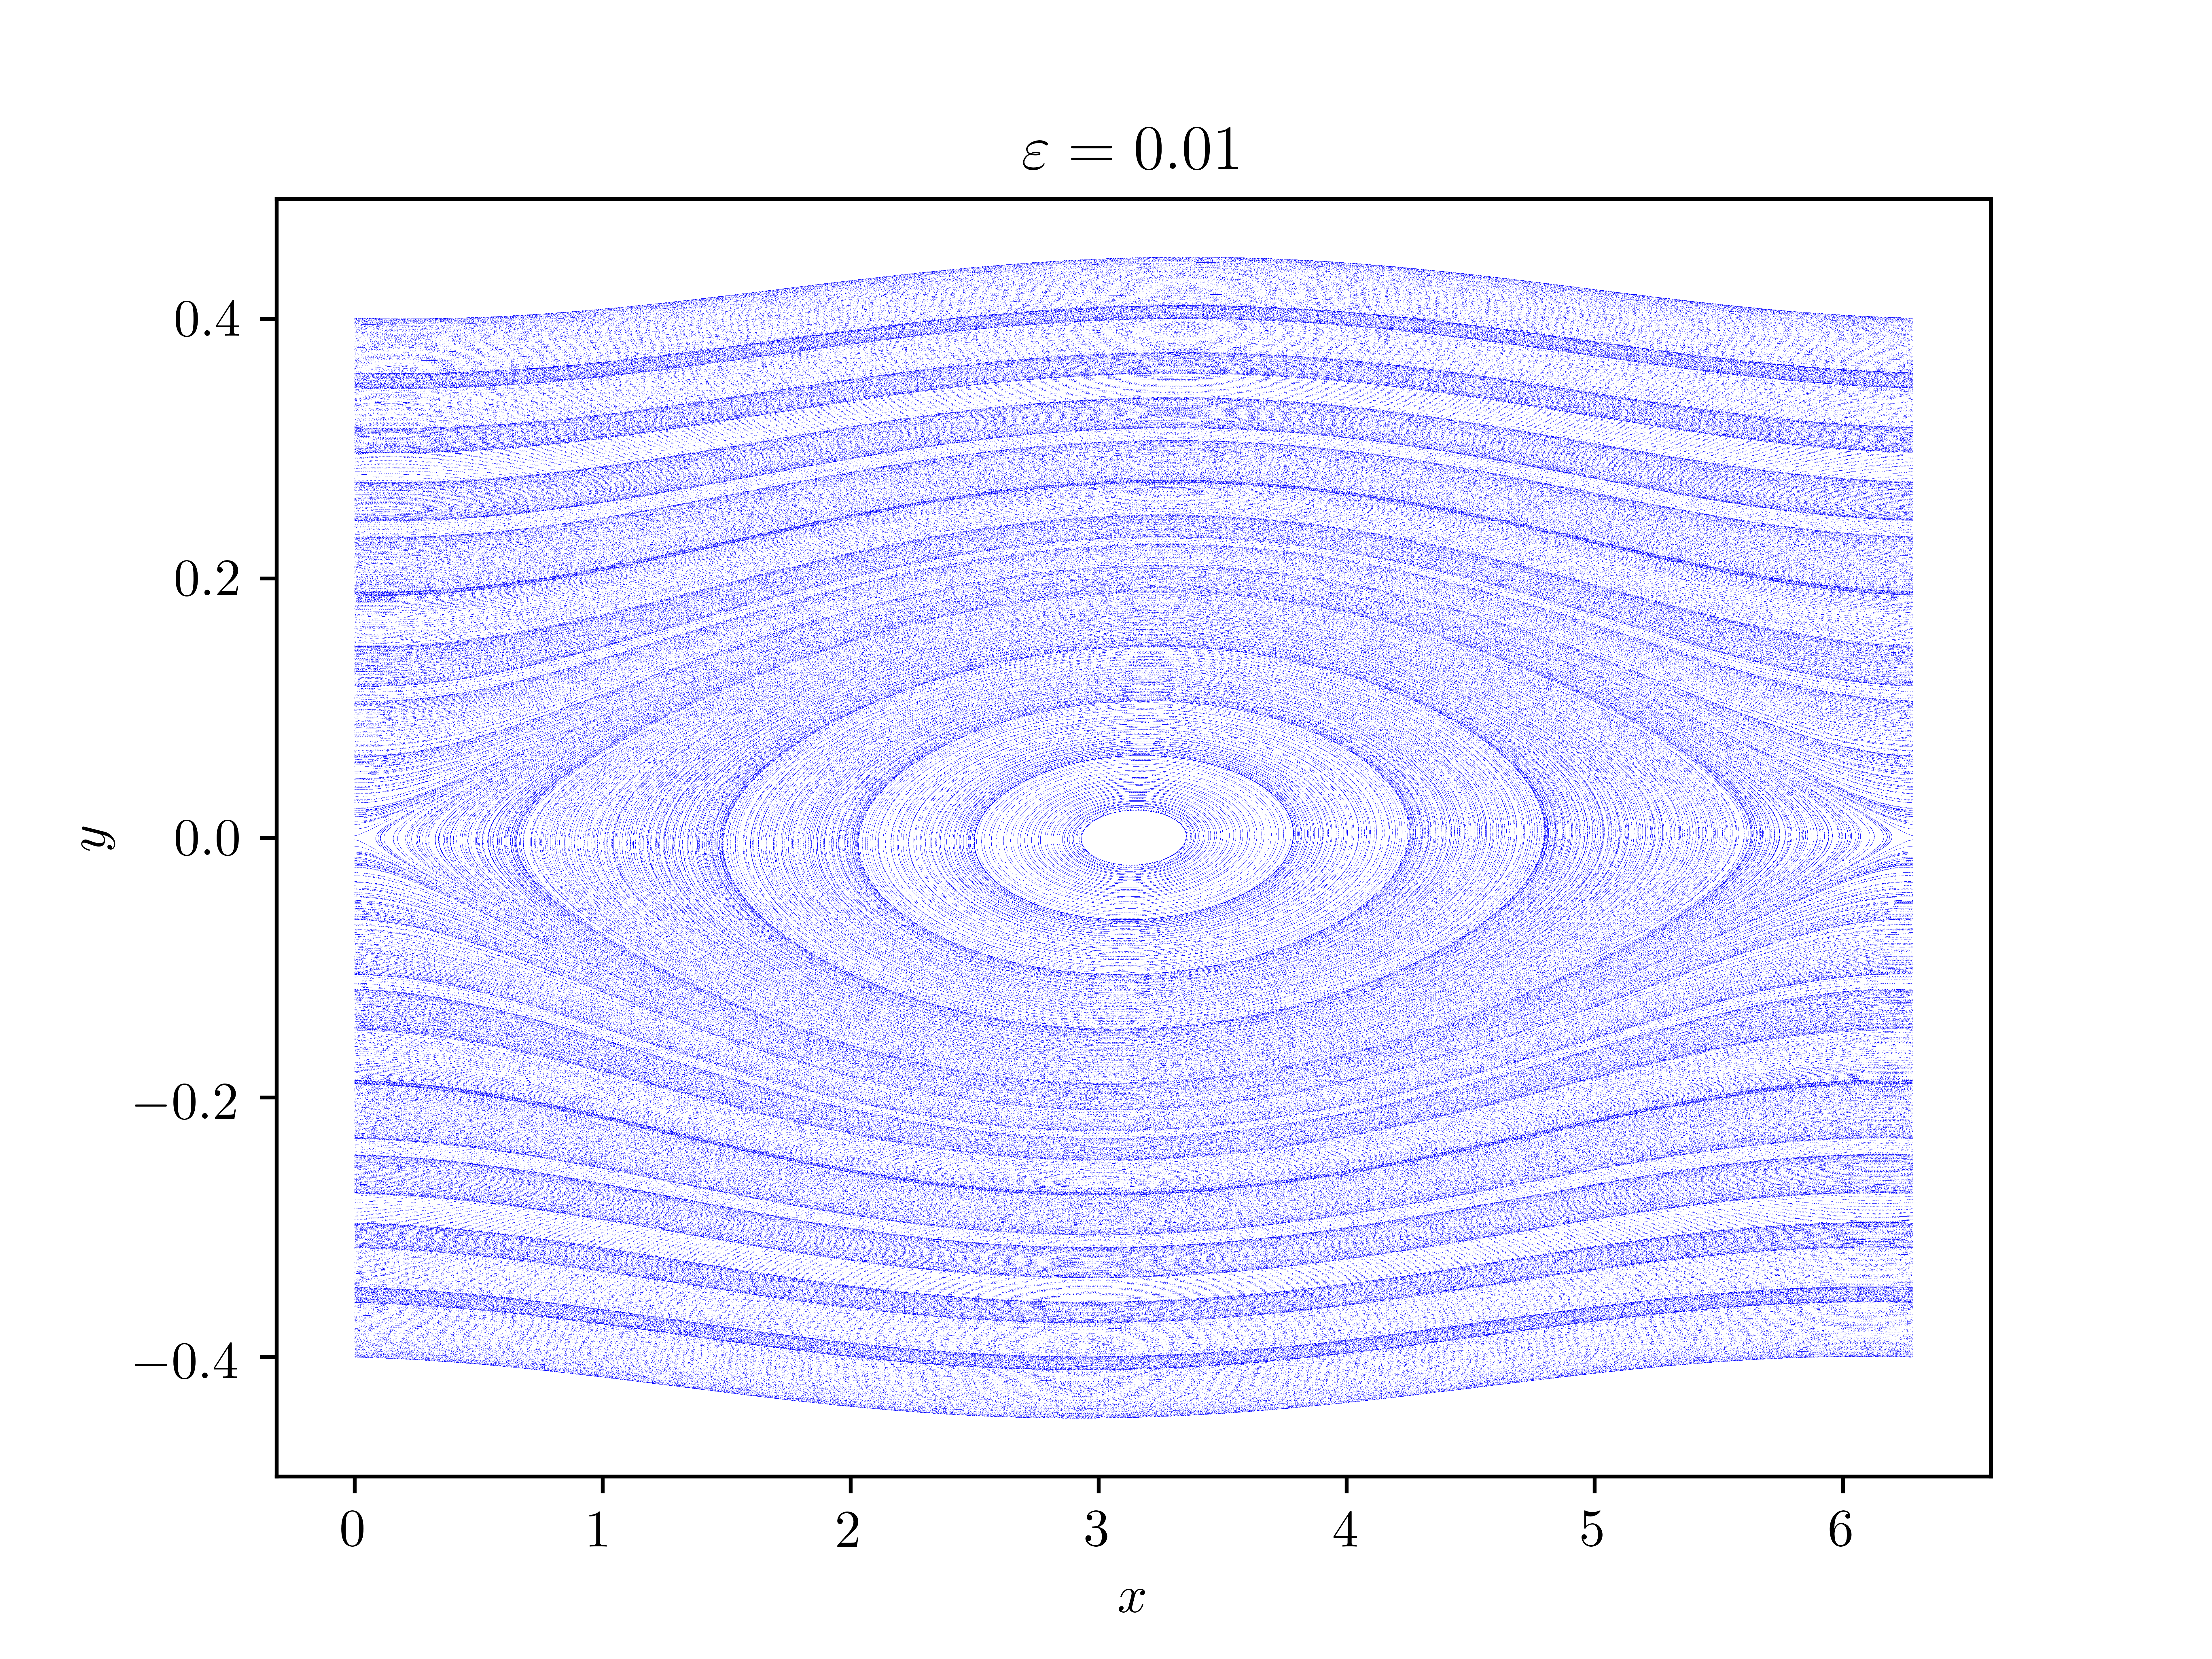
\includegraphics[width=0.5\textwidth]{img/standard-map/sm0}%
		} 
		\subfloat{%
			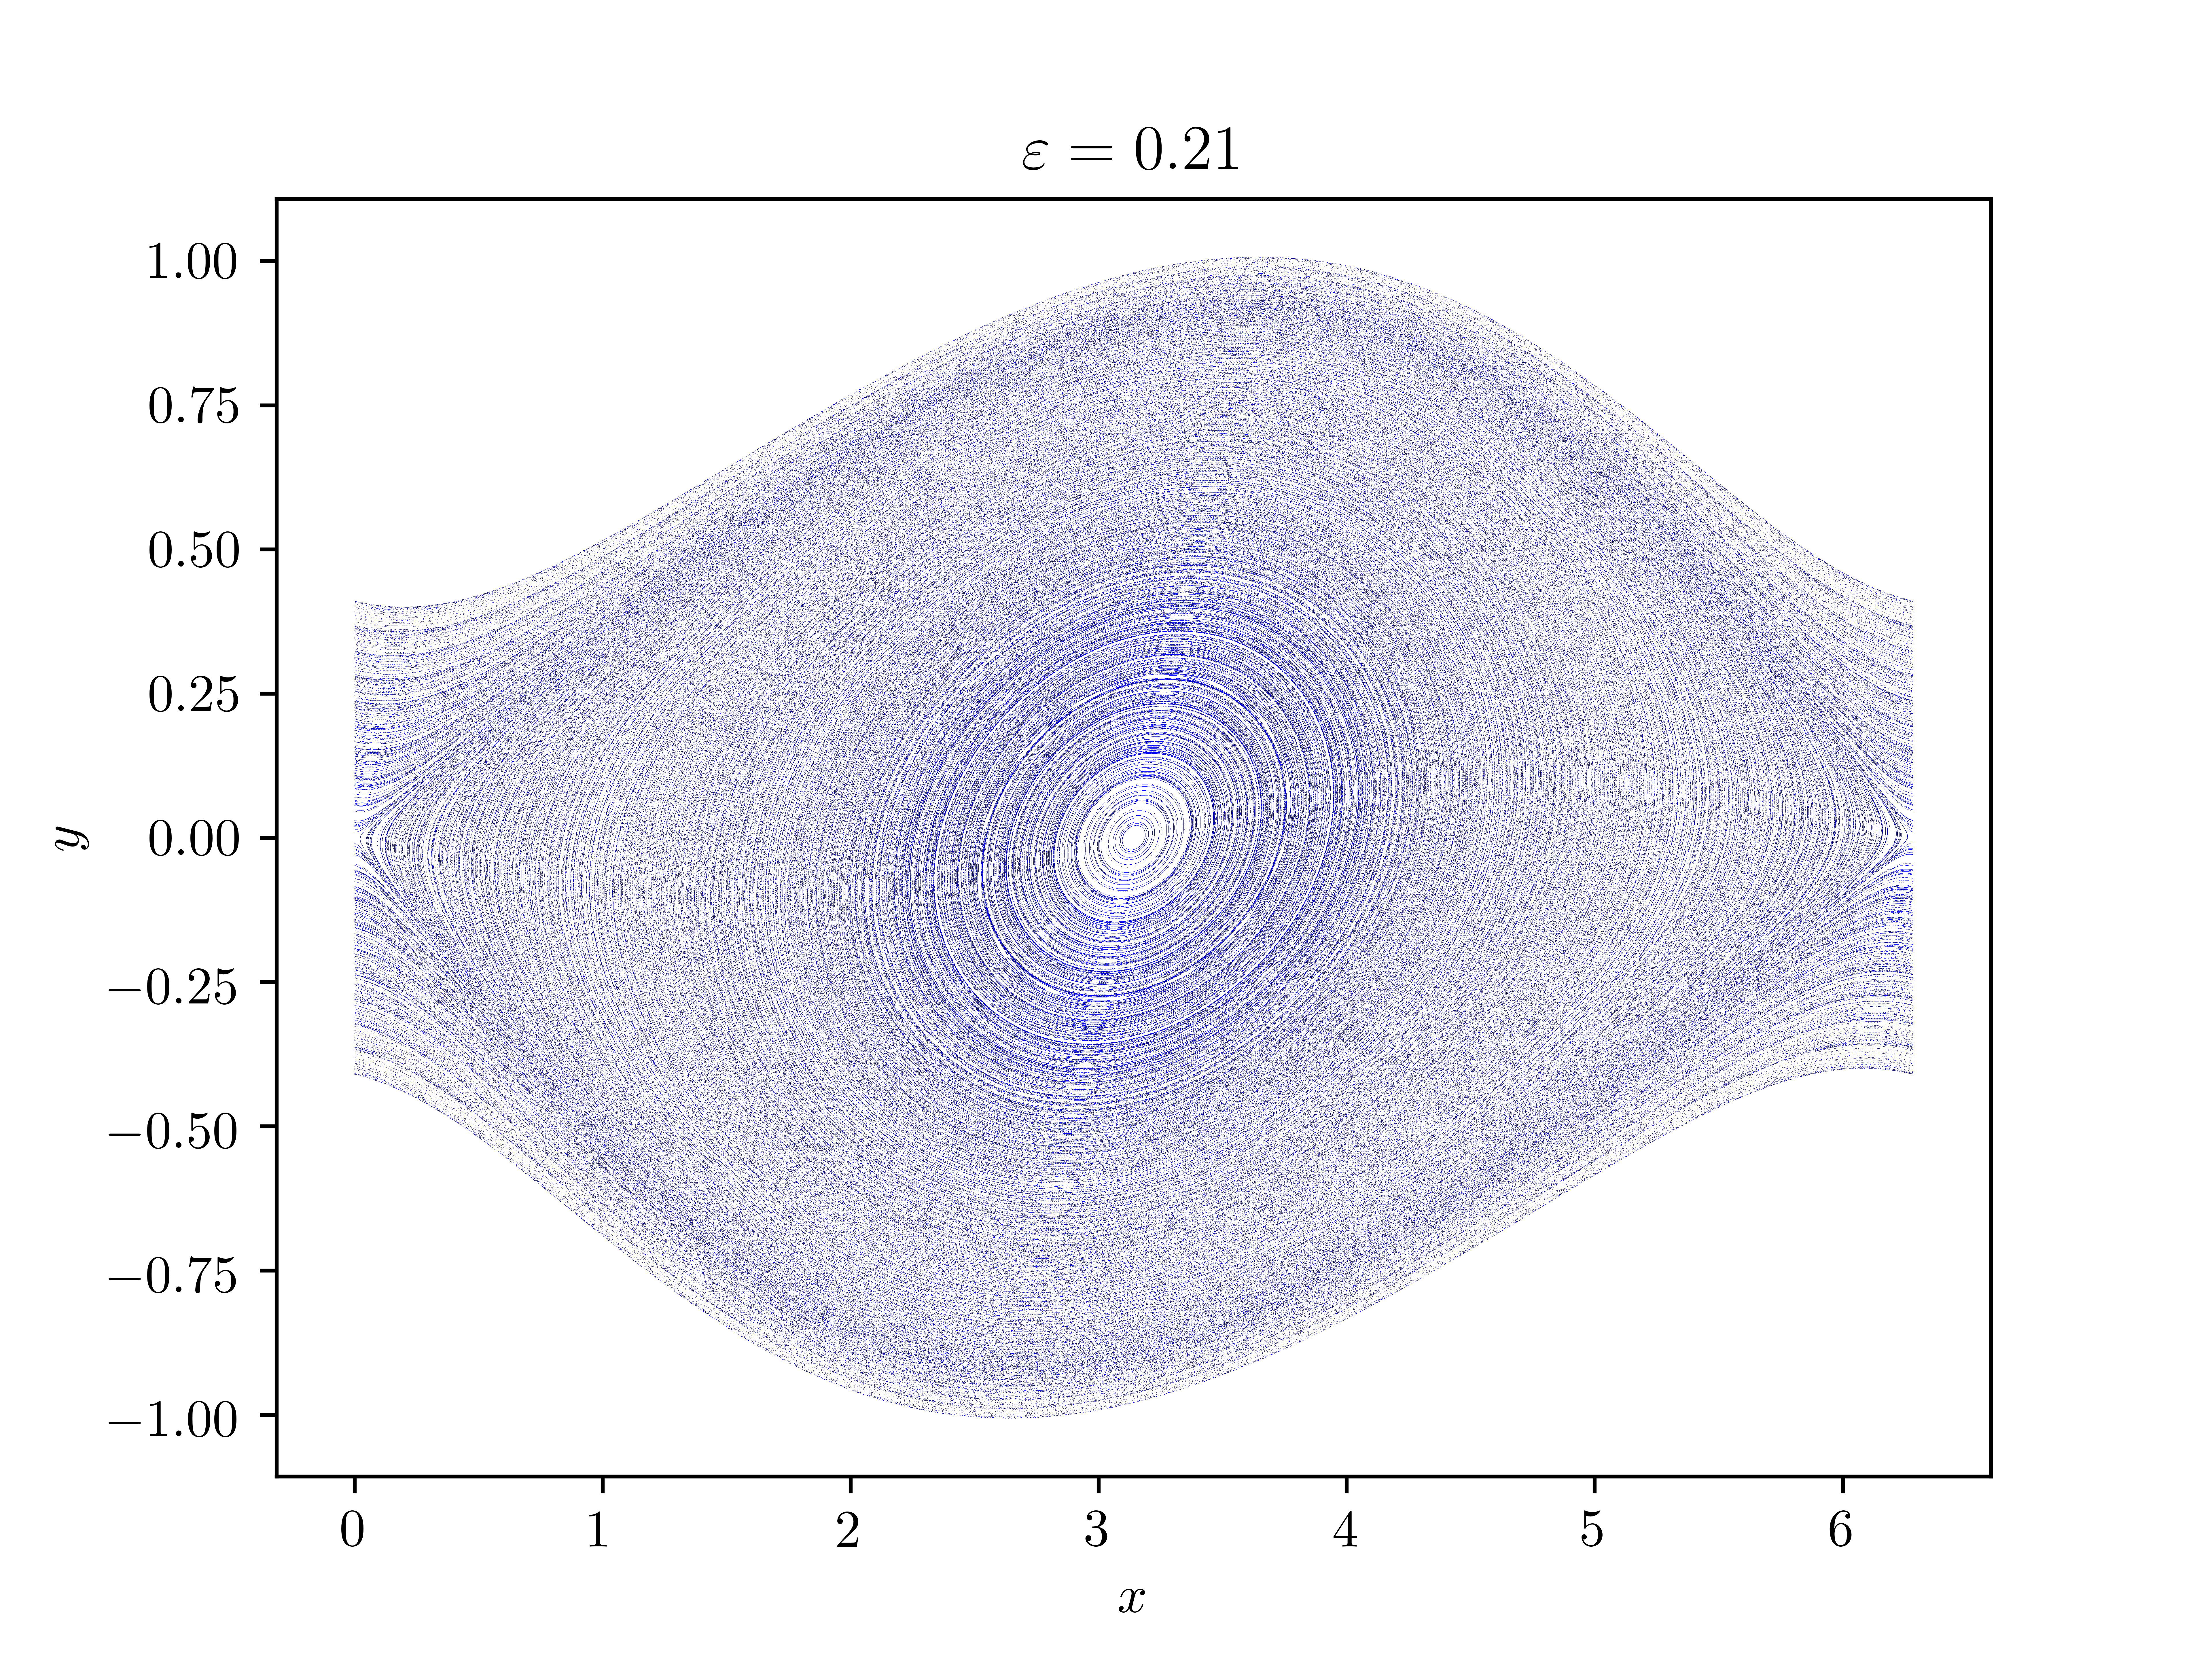
\includegraphics[width=0.5\textwidth]{img/standard-map/sm1}%
		} \hfill
		\subfloat{%
			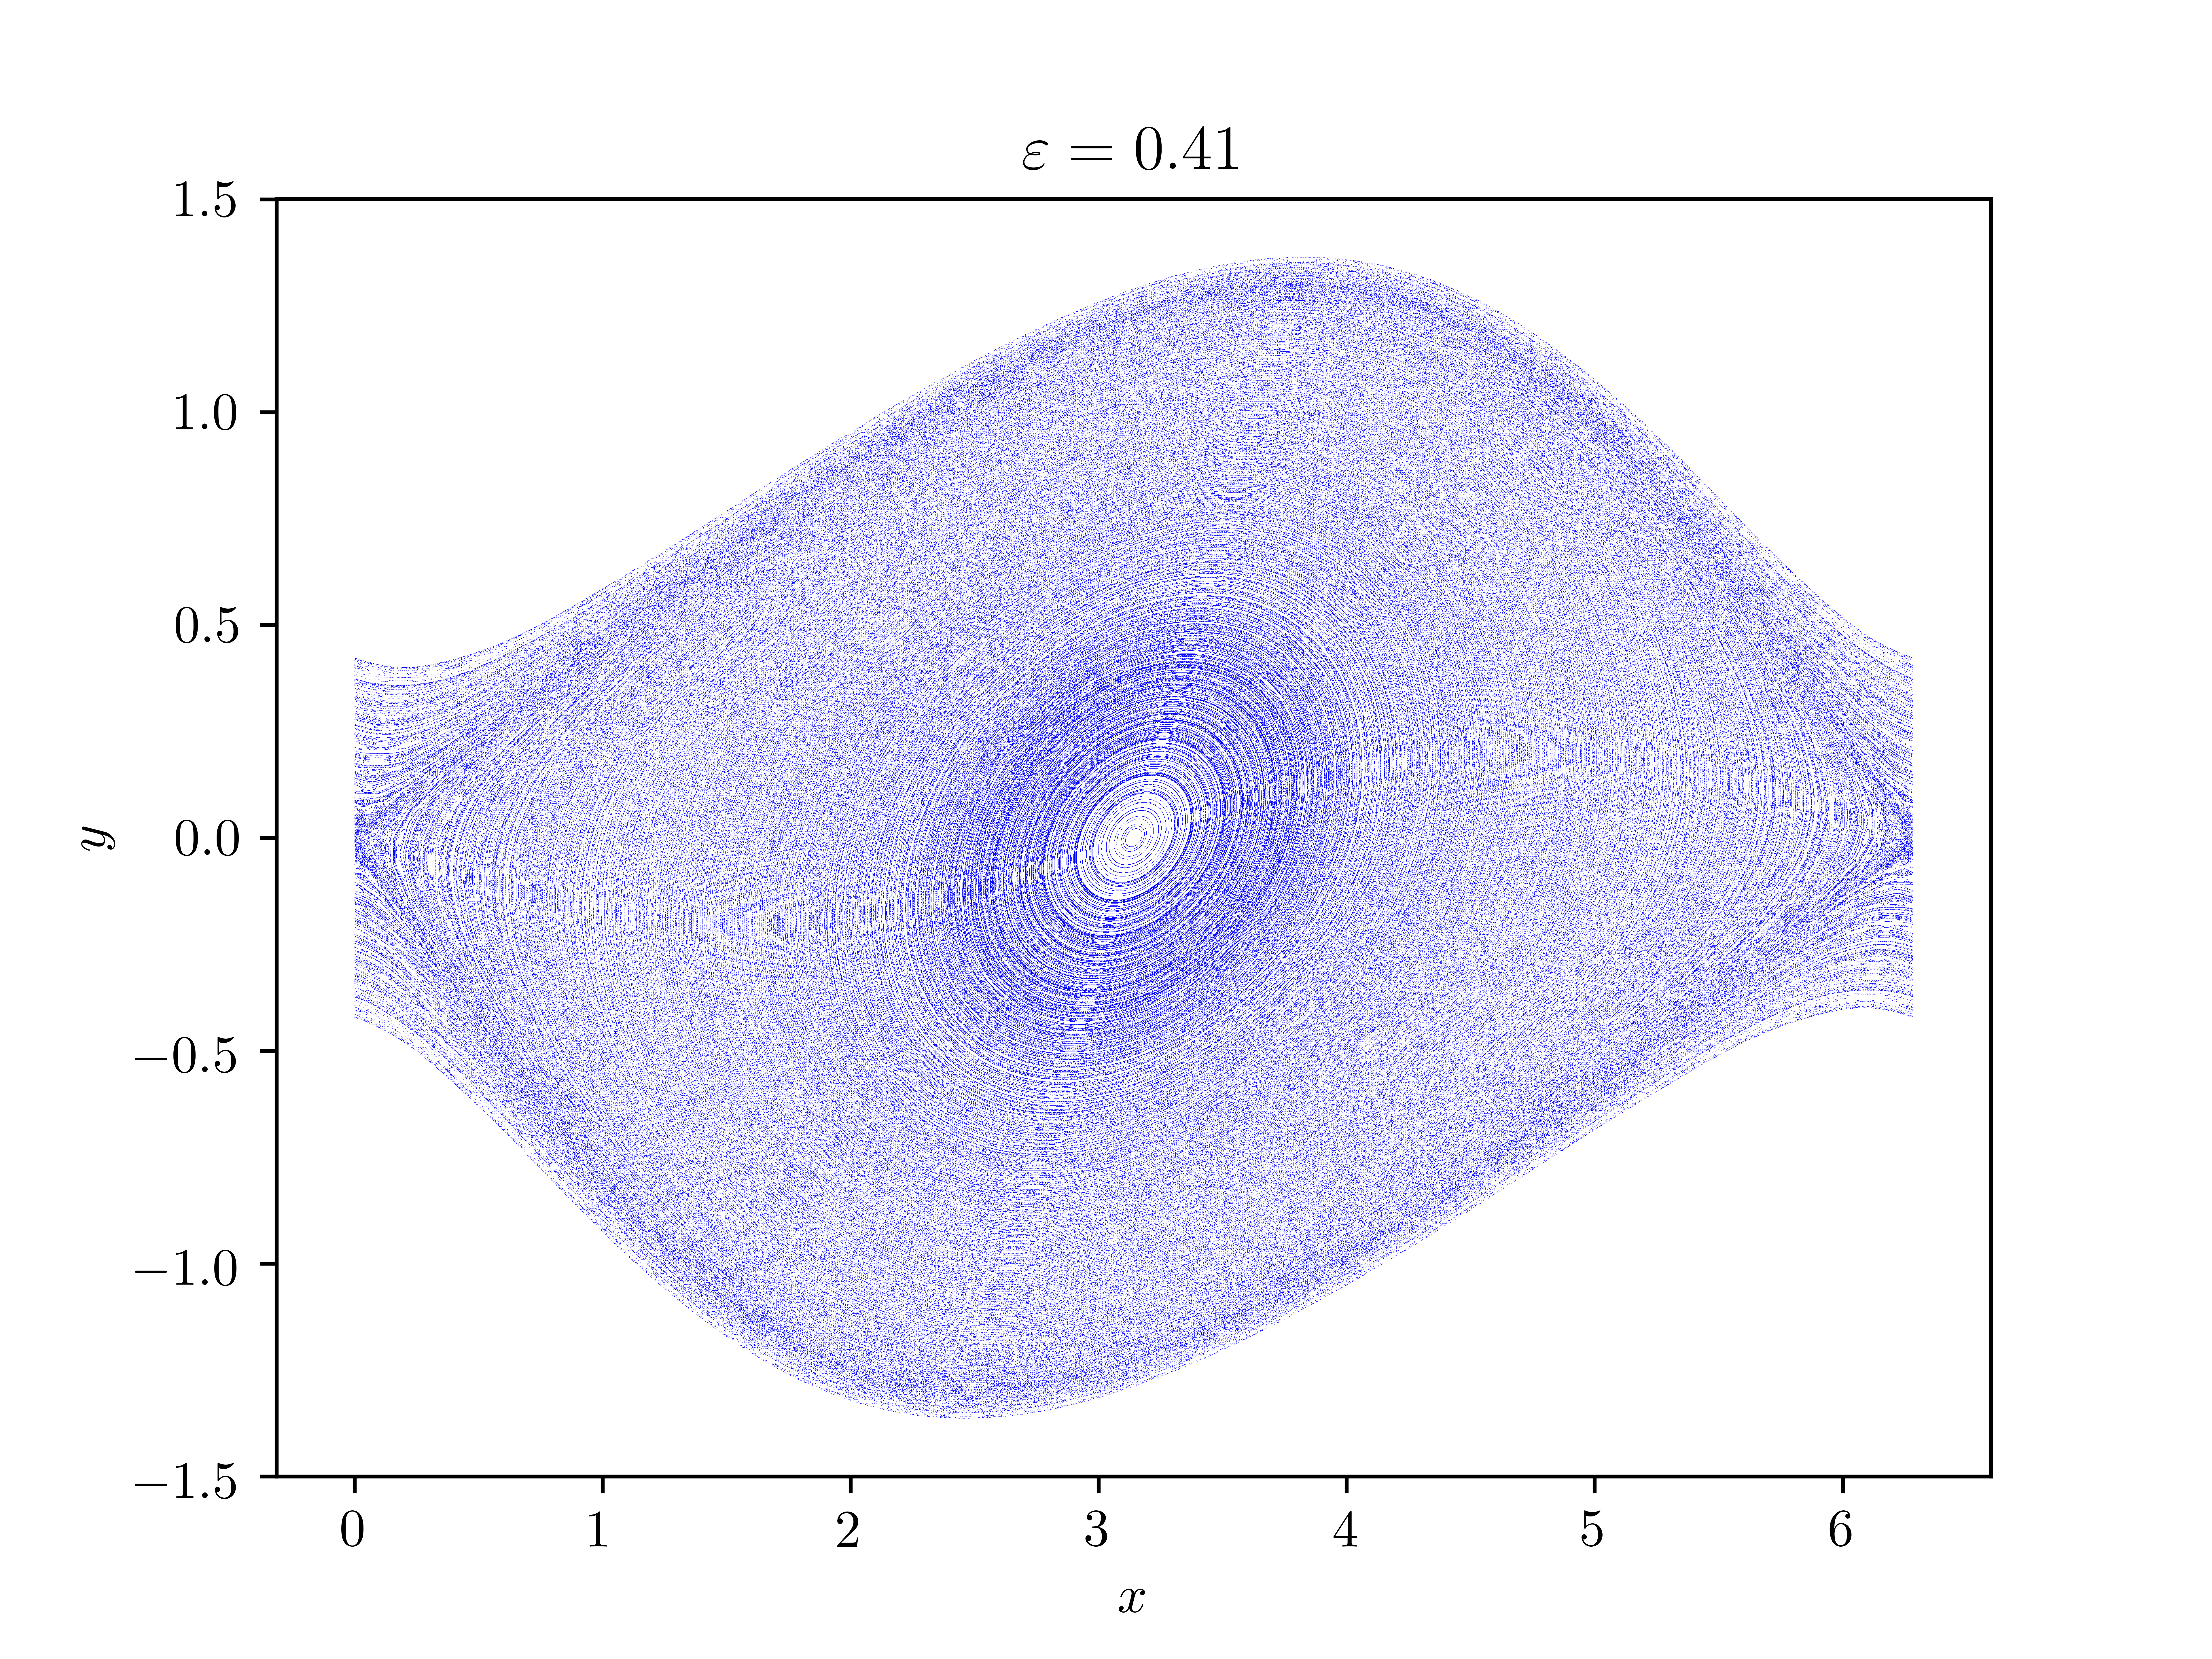
\includegraphics[width=0.5\textwidth]{img/standard-map/sm2}%
		} 
		\subfloat{%
			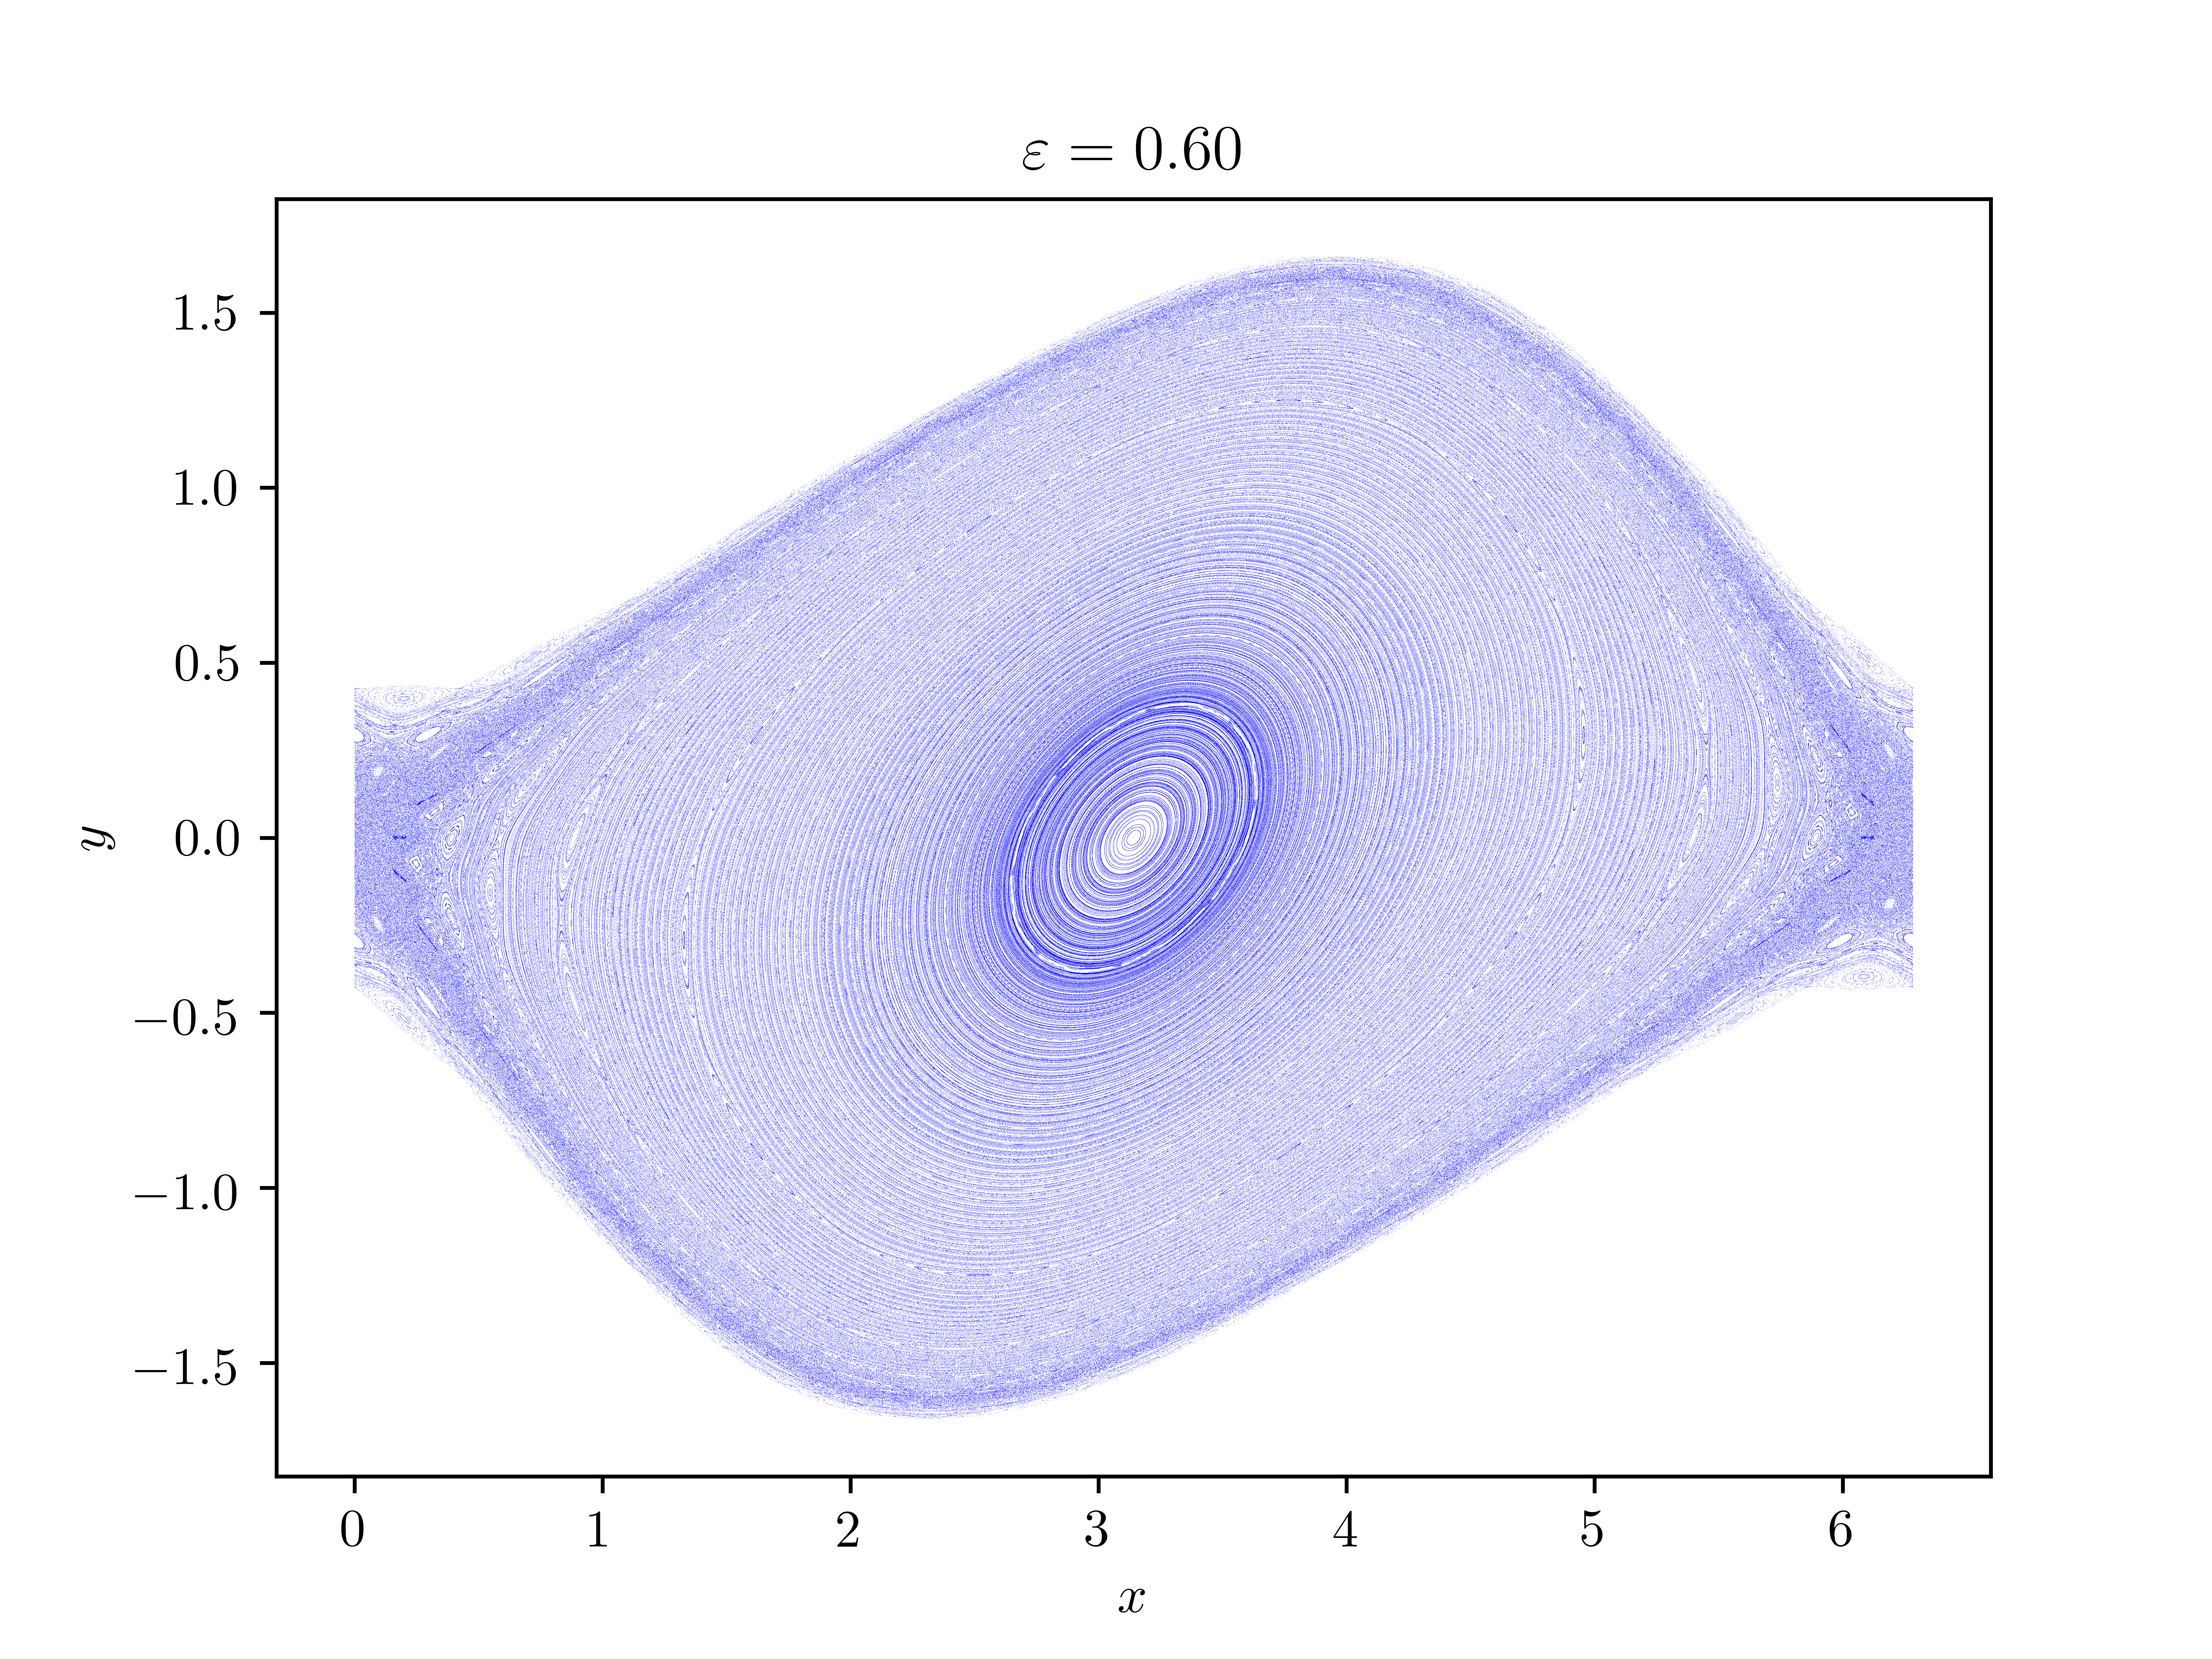
\includegraphics[width=0.5\textwidth]{img/standard-map/sm3}%
		} \hfill
		\subfloat{%
			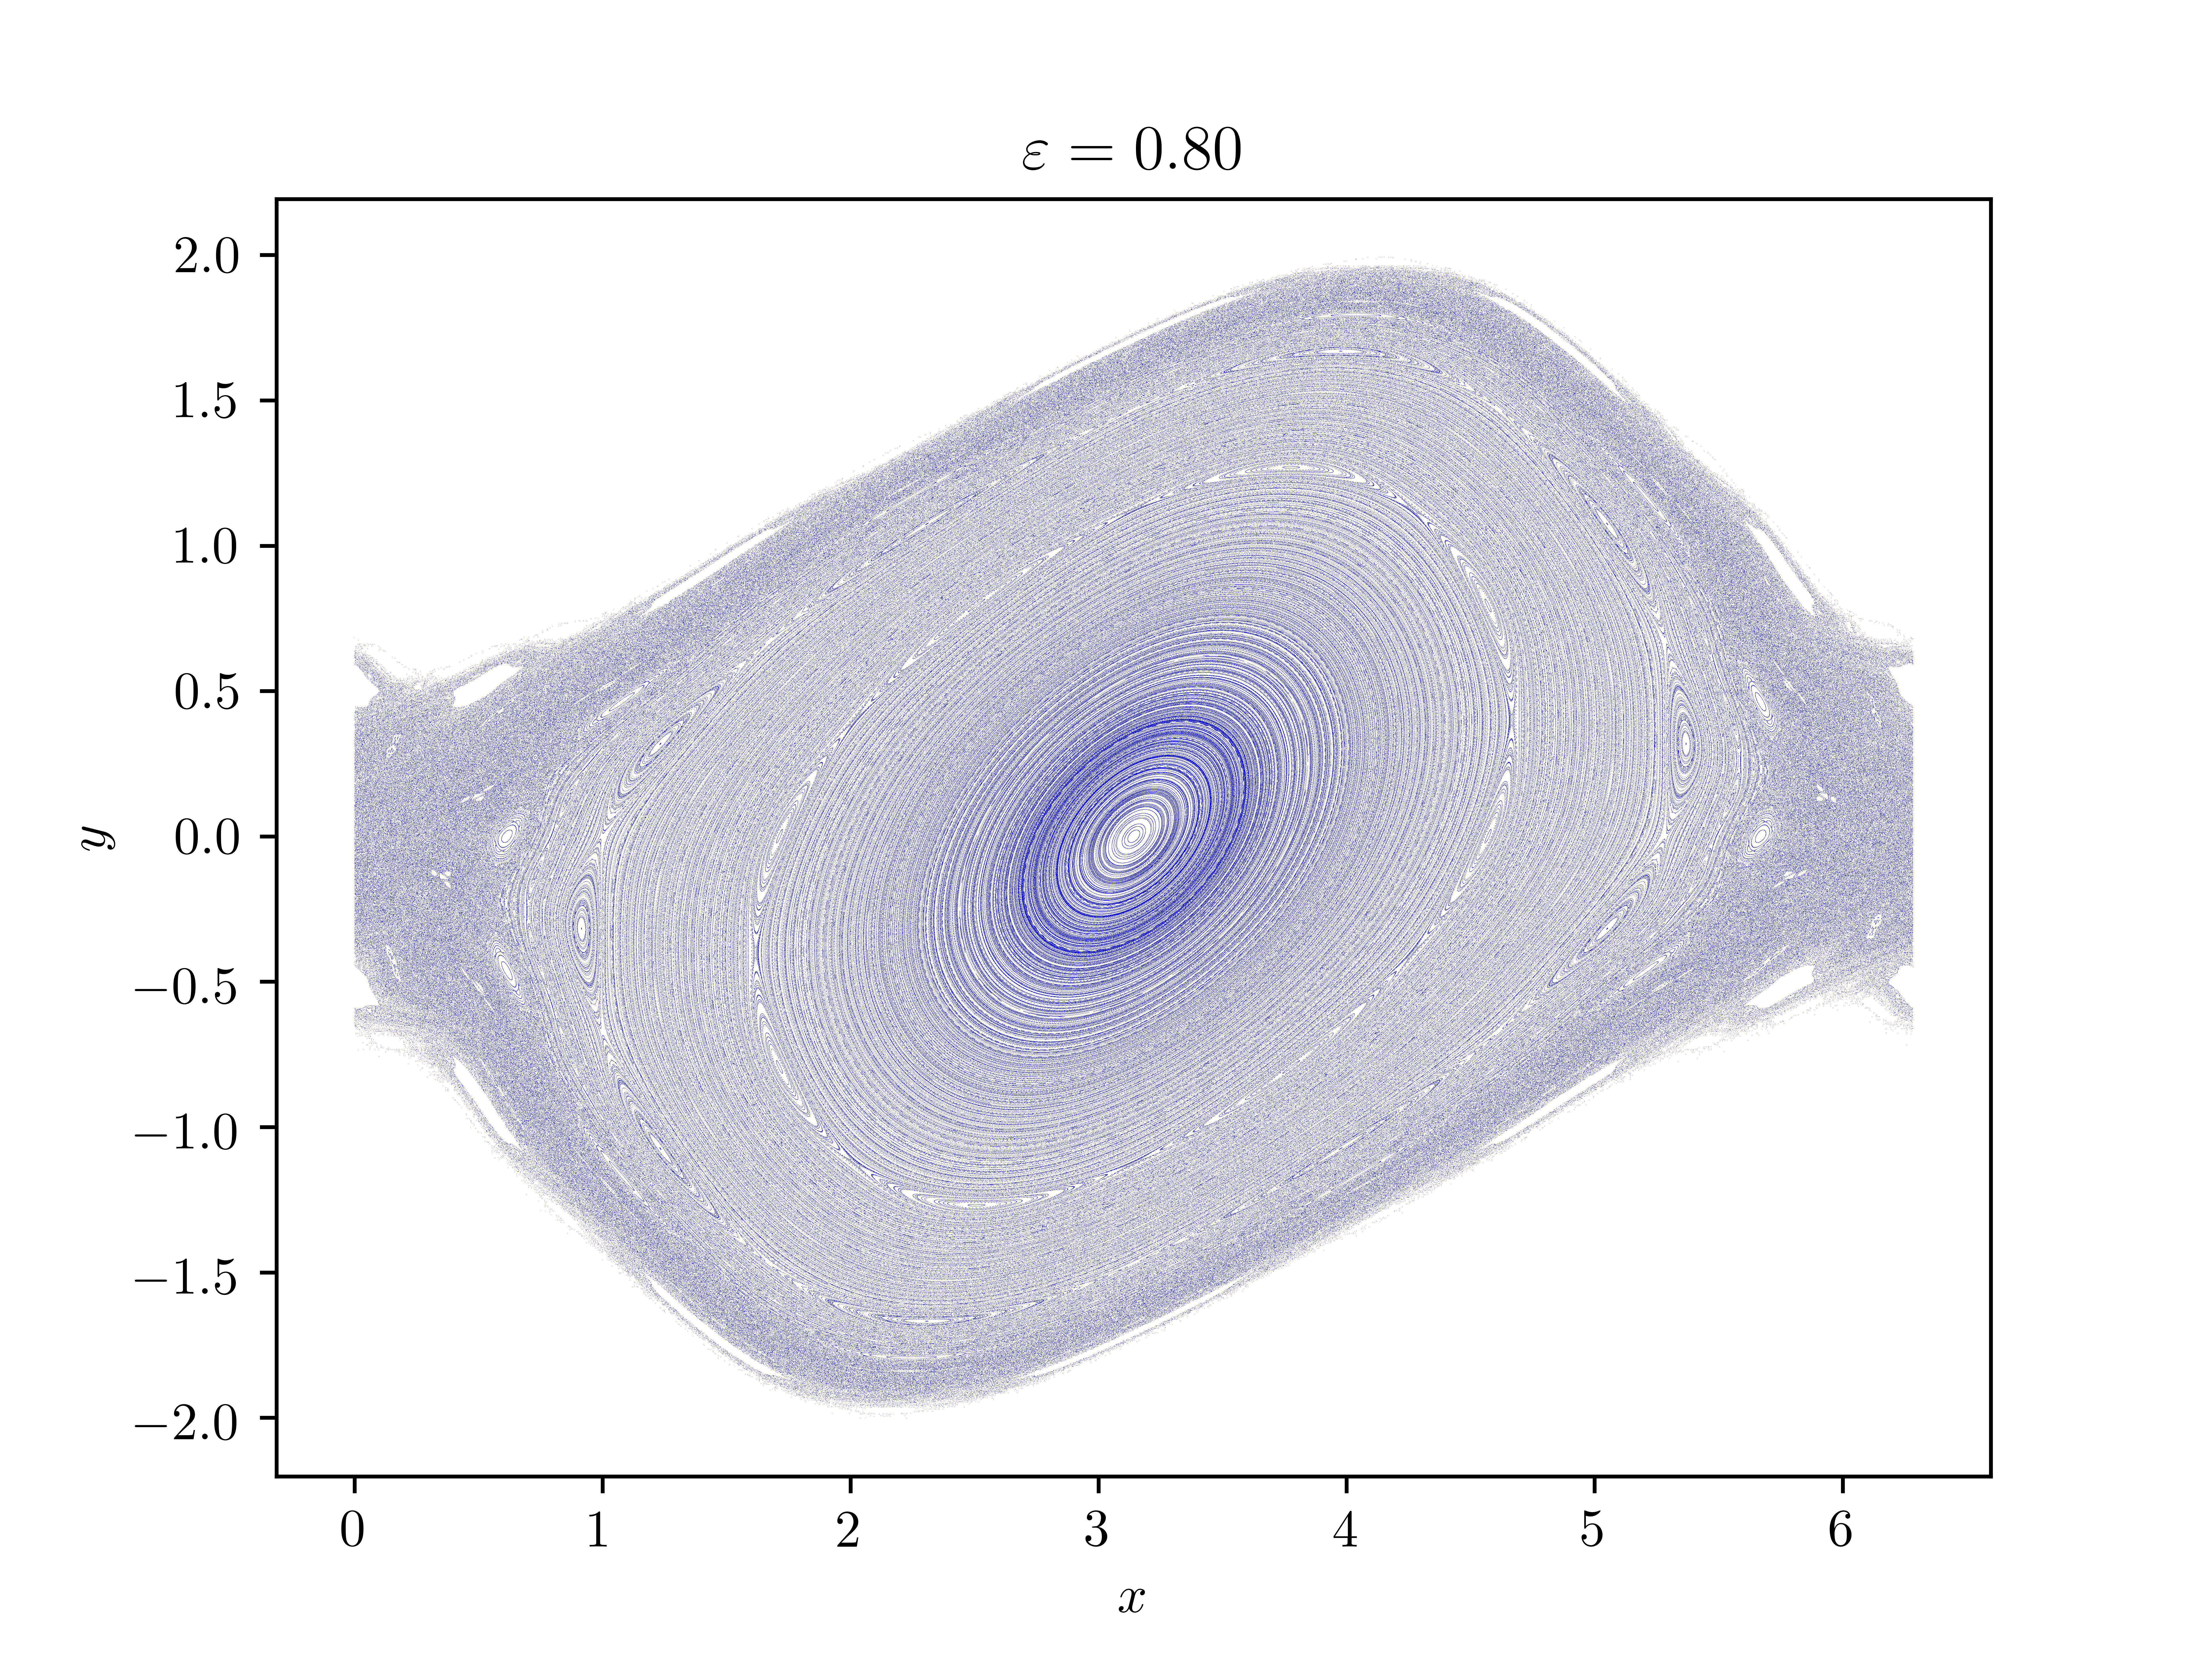
\includegraphics[width=0.5\textwidth]{img/standard-map/sm4}%
		} 
		\subfloat{%
			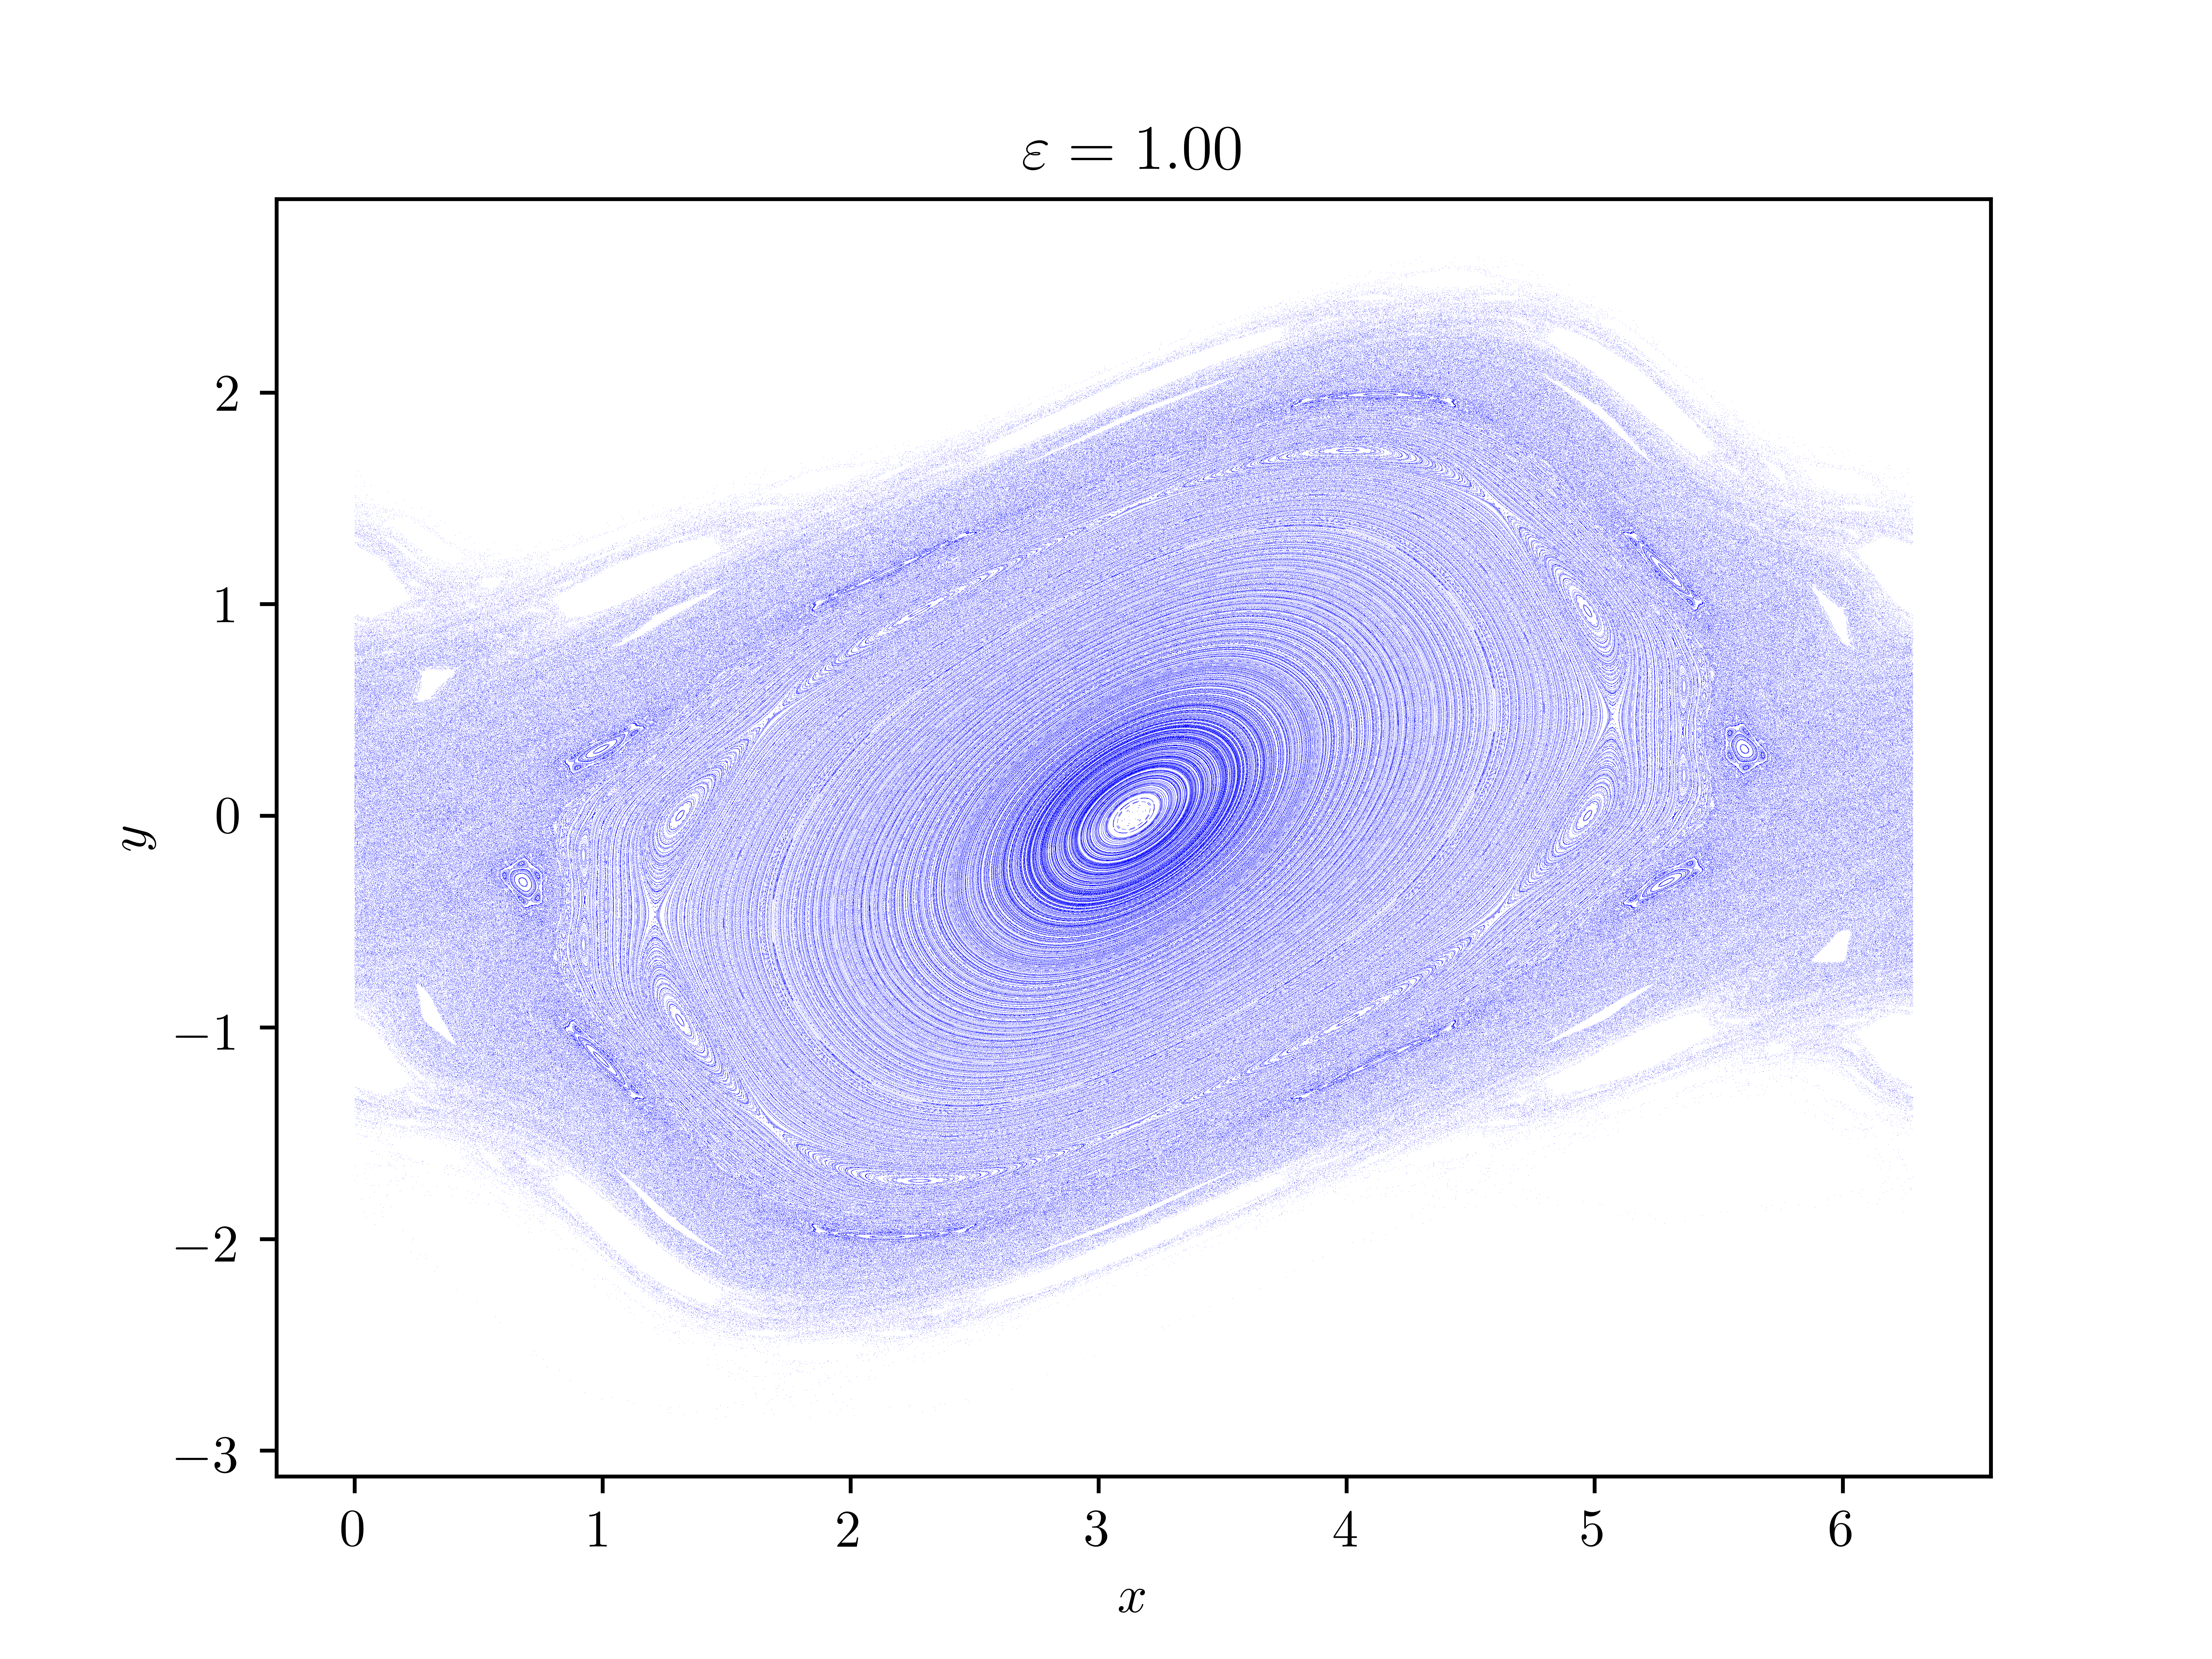
\includegraphics[width=0.5\textwidth]{img/standard-map/sm5}%
		} \hfill
		\caption{Equazione del pendolo discretizzazione per diversi valori di $ \epsilon $}
		\label{fig:pendolo-ode-num}
	\end{figure}
	\fi
	
\end{example}

\section{Lezione del 10/10/2018 [Grotto]}
\subsection{Introduzione}
La Teoria della Misura nasce a inizio '900 per formalizzare la probabilità e per cercare di fondare una teoria dell'integrazione che risulti più efficace di quella di Riemann. Per alcuni sottoinsiemi di $\R$, in particolare per gli intervalli limitati, abbiamo un concetto intuitivo di ``misura'', ovvero la lunghezza dell'intervallo:
\[ \lambda\left([a,b]\right) = b-a. \]
L'obiettivo della teoria della misura è estendere questa nozione ad altri sottoinsiemi di $\R$ in modo coerente, ovvero in modo da rispettare, ad esempio, la proprietà di additività:
\[ A \cap B = \emptyset \Rightarrow \lambda(A\cup B) = \lambda(A) + \lambda(B) \]

Sia $X$ un insieme, $\mathscr{P}(X)$ l'insieme delle parti di X.

\begin{definition}
	$\mathcal{A} \subseteq \mathscr{P}(X)$ è detto \emph{anello} se è chiuso per intersezione, unione e differenza:
	\[ \forall A, B \in \mathcal A \quad A\cup B,\ A\cap B,\ A\smallsetminus B \in \mathcal{A} \]
\end{definition}

\begin{definition}
	$\mathcal{A}$ è un'\emph{algebra} se $X\in \mathcal{A}$.
\end{definition}

\begin{definition}
	$\mathcal{F} $ è una \emph{$\sigma$-algebra} se è un'algebra ed è chiusa per unione numerabile:
	\[ \forall (A_n)_{n\in\N}\subseteq \mathcal{F},\ \bigcup_{n\in \N} A_n \in \mathcal{F} \]
\end{definition}

\begin{exercise}
	Dimostrare che intersezioni di anelli, algebre, $\sigma$-algebre sono ancora rispettivamente anelli, algebre e $\sigma$-algebre.
\end{exercise}

\begin{definition}
	Dato $C\subseteq \mathscr{P}(X)$, la $\sigma$-algebra generata da $C$ è:
	\[ \sigma(C)= \left\{\bigcap \mathcal{F}: \mathcal{F} \text{ è una $\sigma$-algebra} \wedge C\subseteq \mathcal{F} \right\} \]
\end{definition}

\begin{definition}
	Sia $\mathcal{A}$ anello e sia data una funzione $\mu:\mathcal{A} \rightarrow[0,+\infty]$. Allora:
	\begin{itemize}
		\item $\mu$ è \emph{additiva} se $\forall A,B \in \mathcal{A}, A\cap B=\varnothing,\ \mu( A\cup B)=\mu(A)+\mu(B)$;
		\item $\mu$ è \emph{$\sigma$-additiva} se $\forall (A_n)_{n\in\N}\subseteq \mathcal{A}, \forall i\neq j \in \N \ A_i\cap A_j =\varnothing$, allora chiamato $ A=\bigcup\limits_{n\in\N}A_n$ si ha $\mu(A)=\sum\limits_{n\in\N} \mu(A_n)$.
	\end{itemize}
\end{definition}

\begin{oss}
	Se $\mu$ è additiva, $\mu(\varnothing)=\mu(\varnothing)+\mu(\varnothing)$ da cui $\mu(\varnothing)=0$.
\end{oss}

\subsection{Spazi di misura}
\begin{definition}
	Si chiama \emph{spazio di misura} una terna $(X,\mathcal{F}, \mu)$ dove $X$ è un insieme, ${\mathcal{F}\subseteq \mathscr{P}(X)}$ una $\sigma$-algebra e $\mu\colon\mathcal{F} \to [0,+\infty]$ è $\sigma$-additiva. $\mu$ viene detta \emph{misura} e gli insiemi di $\mathcal{F}$ vengono detti \emph{misurabili}.
	Inoltre:
	\begin{itemize}
		\item Se $\mu(X)<+\infty$, allora $\mu$ viene detta \emph{misura finita}. Questo implica che $\forall A \in \mathcal{F}, {\mu(A) < +\infty} $;
		\item Se $\mu(X)=1$ allora $\mu$ viene detta \emph{probabilità};
		\item Se $\exists (A_n)_{n\in\N}\subseteq\mathcal{F} : \bigcup\limits_{n\in\N}A_n=X$ e $\forall n \in\N \ \mu(A_n) <+\infty$, allora $\mu$ si dice \emph{$\sigma$-finita}.
	\end{itemize}
\end{definition}
Introduciamo le seguenti notazioni:
\[ A_n \uparrow   A \text{ se } \forall n \in\N \ A_n \subseteq A_{n+1} \text{ e } \bigcup\limits_{n\in \N}A_n = A \]
\[ A_n \downarrow A \text{ se } \forall n \in\N \ A_n \supseteq A_{n+1} \text{ e } \bigcap\limits_{n\in \N}A_n = A \]
Dato $(A_n)_{n\in\N}$, si definiscono $\underset{n\to+\infty}{\liminf}A_n \coloneqq\underset{n\in\N}{\bigcap}\underset{k\geq n}{\bigcup}A_k$ l'insieme di tutti gli elementi che appaiono frequentemente tra gli $A_n$, e $\underset{n\to +\infty}{\limsup}A_n\coloneqq\underset{n\in\N}{\bigcup}\underset{k\geq n}{\bigcap}A_k$ l'insieme di tutti gli elementi che appaiono definitivamente tra gli $A_n$.

\begin{exercise}
	Data $\mu$ additiva su $\mathcal{A}$ anello, $\mu$ è $\sigma$-additiva se e soltanto se $\forall A_n \uparrow A$ con $\forall n\; A_n,A \in \mathcal{A}$ $\mu(A)=\lim_{n\to +\infty} \mu(A_n)$.
\end{exercise}
\begin{exercise}
	Data $\mu$ $\sigma$-additiva su $\mathcal{A}$ anello, allora $\forall A_n \downarrow A$ con $\forall n\; A_n,A \in \mathcal{A}$ e $\mu(A_n) < + \infty$ definitivamente, vale $\mu(A)=\lim_{n\rightarrow +\infty} \mu(A_n)$.
\end{exercise}
\begin{exercise}
	Dato $(X,\mathcal{F}, \mu)$ spazio di misura, $\forall (A_n)_{n\in\N}\subseteq\mathcal{F}$  si ha $\mu\left(\underset{n\rightarrow +\infty}{\liminf} A_n\right) \leq \underset{n\rightarrow +\infty}{\liminf} \mu (A_n)$. Inoltre se $\mu\left(\underset{n\in\N}{\bigcup} A_n <+\infty\right)$, allora $\mu\left(\underset{n\rightarrow +\infty}{\limsup} A_n\right) \leq \underset{n\rightarrow +\infty}{\limsup} \mu (A_n)$.
\end{exercise}
\begin{exercise}[Borel-Cantelli]
	Se $\sum\limits_{n\in\N} \mu(A_n) < +\infty$, allora $\mu\left(\underset{n\rightarrow +\infty}{\limsup} A_n\right)=0$.
\end{exercise}
\begin{example}
	Dato $X$ insieme, $\mathcal{F}\subseteq \mathscr{P}(X)$ una $\sigma$-algebra, sono esempi di misure:
	\begin{itemize}
		\item \emph{Misura finita}: se $A$ è finito allora $\mu(A)=\card{A}$, altrimenti $\mu(A)=+\infty$;
		\item \emph{Misura di Dirac}: Dato $x\in X$, se $x\in A$ allora $\delta_x(A)=1$, altrimenti $\delta_x(A)=0$;
		\item Definita la \emph{$\sigma$-algebra dei singoletti} di $ X $ come:
		\[ \mathcal{F} \coloneqq \sigma\left( \left\{ \{x\} : x\in X \right\} \right) = \left\{ A\subseteq X : A \text{ o } X\smallsetminus A \text{ è al più numerabile} \right\} \]
		Supponiamo $ X $ sia più che numerabile. Poniamo: $ \mu(A) = 0 $ se $ A $ è al massimo numerabile, $ \mu(A) = +\infty $ altrimenti. 
		Allora per ogni sequenza $(A_n)_{n\in\N}\subseteq\mathcal{F},\ \bigcup_{n\in\N} A_n=X$, almeno uno degli $A_n$ deve essere più che numerabile, quindi la sua misura è $+\infty$ e pertanto $ \mu $ è una misura non $ \sigma $-finita.
	\end{itemize}
\end{example}
\begin{example}
	Prendendo $X=\N,\ \mathcal{F} =\mathscr{P}(\N)$, si possono definire le distribuzioni di probabilità discrete e le relative misure. Data una funzione di probabilità $p: \N \rightarrow [0,+\infty)$ che soddisfi $\sum_{n\in\N} p(n)=1$, questa induce una misura $\mu$ definita come $\mu(A)=\sum_{n\in A} p(n)$. Esempi sono:
	\begin{itemize}
	\item Distribuzione di Bernoulli di parametro $0<q<1$: $p(0)=1-q$, $p(1)=q$, $p(n)=0$ per $n\geq 2$;
	\item Distribuzione Binomiale di parametro $0<q<1$: $\displaystyle p(k)=\binom{n}{k} q^k (1-q)^{n-k}$;
	\item Distribuzione di Poisson di parametro $\lambda\in\R$: $\displaystyle p(n)=\frac{\lambda^ne^{-\lambda}}{n!}$.
	\end{itemize}
\end{example}
\begin{proposition}
	Sia $(X,\mathcal{F}, \mu)$ uno spazio di misura e sia $\mathcal{E} \subseteq \mathcal{F}$ una sotto-$\sigma$-algebra, allora $\mu\lvert_{\mathcal{E}}$ è una misura di $(X,\mathcal{E})$.
\end{proposition}
\begin{definition}
	Se $Y\subseteq X$, la \emph{sotto $\sigma$-algebra di sottoinsiemi} di $Y$ è $\mathcal{E}_Y=\{A\in \mathcal{F} : A \subseteq Y\}$.
\end{definition}
\begin{exercise}
	$\mu\lvert_{Y}(A)=\mu\lvert_{\mathcal{E}_Y}(A)$. Inoltre se $Y$ è misurabile (cioè $Y\in \mathcal{F}$), allora questo è uguale a $\mu(A\cap Y)$.
\end{exercise}
\begin{definition}
	Dato $(X,\mathcal{F}, \mu)$ uno spazio di misura, se per $A\in \mathcal{F}$ vale $\mu(A)=0$ allora $A$ si dice \emph{trascurabile}. L'insieme $\mathscr{N}=\left\{A\in \mathcal{F} : \mu(A)=0 \right\}$ è l'insieme di tutti i punti trascurabili. Se una certa proprietà vale $\forall x \in X\smallsetminus \mathscr{N}$ si dice che vale \emph{quasi ovunque} (o \emph{quasi certamente} se $ \mu $ è una probabilità).
\end{definition}

\begin{thm}[Coincidenza delle misure]
	Sia $X$ insieme, $\mathcal{F}$ una $\sigma$-algebra e $\mu, \nu$ due misure su $(X,\mathcal{F})$. Sia $K\subseteq \mathcal{F}, K\neq \varnothing$ con le seguenti proprietà:
	\begin{enumerate}[label=(\roman*)]
	\item $\forall A \in K, \mu(A)=\nu(A)$, cioé $\mu$ e $\nu$ coincidono su tutto $K$;
	\item $K$ è chiuso per intersezioni;
	\item $\sigma(K)=\mathcal{F}$;
	\item\label{th:coin:cusumano} $\exists (X_n)_{n\in \N}\subseteq K, \; X_n \uparrow X$ e $\forall n\; \mu(X_n)=\nu(X_n)<+\infty$.
	\end{enumerate}
Allora $\mu$ e $\nu$ coincidono su tutto $\mathcal{F}$.
\end{thm}
\begin{exercise}
	Trovare un controesempio al teorema se non vale il punto \ref{th:coin:cusumano}, ovvero $X, \mathcal{F} \supseteq K$ e due misure $\mu,\nu$ che coincidano su $K$ ma non su tutto $\mathcal{F}$.
\end{exercise}
\begin{thm}[Estensione di Carathéodory]
	Sia $X$ insieme e $\mathcal{A}\subseteq \mathscr{P}(X)$ un anello. Se $\mu\colon\mathcal{A}\to[0,+\infty]$ è $\sigma$-additiva, esiste un'estensione di $\mu$ ad una misura $\tilde\mu$ su $\sigma(\mathcal{A})$. Inoltre se l'estensione $\tilde\mu$ è $\sigma$-finita, allora essa è unica.
\end{thm}
\begin{example}
	Siano $ X = \R $ e $ \mathcal{A} $ l'anello generato dagli intervalli della forma $[a,b)$. Sia:
	\[ \mu\left( \bigcup_{i=1}^N [a_i,b_i) \right) \coloneqq \sum_{i=1}^N (b_i-a_i) \]
	Per il teorema di Carathéodory, esiste una misura $\lambda$ su $\sigma(\mathcal{A})=\sigma(\tau)$\footnote{Data una topologia $ \tau $, $ \mathcal{B} \coloneqq \sigma(\tau) $ è detta \emph{$ \sigma $-algebra dei Boreliani}.} che estende $\mu$.
\end{example}

\begin{definition}
	Dato $(X,\tau)$ spazio topologico, $\sigma(\tau)$ è la $\sigma$-algebra dei Boreliani $\mathcal{B}$.
\end{definition}
\begin{exercise}
	Preso $ (\R,\tau_{\text{eu}}) $, $\card{\mathcal{B}} = |2^{\N}| $.
	\textcolor{red}{Hint: facile per induzione transfinita.}
\end{exercise} 
\begin{exercise}
	Dato $(\R^d, \mathcal{B}, \mu)$ spazio di misura sulla $\sigma$-algebra dei Boreliani, con $\mu$ misura finita sui compatti e invariante per traslazione (ovvero $\forall x \in \R^d,\ \forall A \in \mathcal{B},\ \mu(x+A)=\mu(A)$), allora $\exists c > 0 : \mu=c\lambda$ dove $\lambda$ è la misura di Lebesgue.
\end{exercise}
\begin{exercise}
	È possibile non solo traslare lo spazio, ma anche trasformarlo tramite applicazioni lineari. Sia $T\in\mathrm{GL}(d,\R),\ \phi\colon\R^d \to \R^d,\ \phi(x)=Tx$. Allora $\forall A \in \mathcal{B}$, $ {\lambda(\phi(A))=\lambda(A)\abs{\det T} }$.
	Hint:
	\begin{enumerate}
		\item $\mu\left ([0,1]^d\right )=c\Rightarrow \mu\left ([0, \frac{1}{k}]^d\right )=\frac{c}{k^d}\Rightarrow \mu=c\lambda$ su $\mathcal{A}$, usare il teorema sopra {\color{red}[NOTA: quale dei due?]};
		\item Se $\mathbb{T} \in \mathrm{GL}(n,\R)$, allora esistono $P_1, P_2$ ortogonali e $D$ diagonale tali che $\mathbb{T}=P_1DP_2$.
	\end{enumerate}
\end{exercise}

\begin{definition}[$ \sigma $-ideale]
	Sia $ (X,\mathcal{F},\mu) $ uno spazio di misura. Diciamo che $ I\subseteq\mathcal{F} $ è un \emph{$ \sigma $-ideale} di $ \mathcal{F} $ se sono soddisfatte le seguenti proprietà:
	\begin{enumerate}[label=(\roman*)]
		\item $ \emptyset\in I $;
		\item $ \forall N\in I,\ A\subseteq N \Rightarrow A \in I $;
		\item $ \left\{A_n \right\}_{n\in\mathbb{N}} \subseteq I \Rightarrow \bigcup\limits_{n\in\mathbb{N}} A_n\in I $.
	\end{enumerate}
\end{definition}

\begin{definition}
	Una misura è \emph{completa} se $ \mathscr{N} $ è $ \sigma $-ideale di $ \mathscr{P}(X) $.
\end{definition}

\begin{thm}[Completamento di Misura]
	Sia $ (X,\mathcal{F},\mu) $ uno spazio di misura. Allora $ \mu $ si estende a una misura completa massimale su:
	\[ \overline{\mathcal{F}} \coloneqq \left\{ A = E \cup N : E\in \mathcal{F},\ N\subseteq N' \in \mathscr{N} \right\} \]
	\textcolor{red}{Siamo sicuri?}
\end{thm}
Dunque la misura sui Boreliani $\big(\R^d, \mathcal{B}, \lambda\big)$ si estende a $\big(\R^d, \mathcal{M}, \tilde\lambda \big)$ con $\tilde\lambda$ completa su \(\mathcal{M}\) insieme dei Lebesgue-misurabili.

\begin{exercise}
	$\card{\mathcal{M}}=|2^{\R}|$.
	Hint: Prendere i sottoinsiemi dell'insieme di Cantor. \textcolor{red}{Difficile per induzione transfinita.}
\end{exercise}
\begin{exercise}[Insieme di Vitali]
	Esiste $V\subseteq \R$, $V\not\in \mathcal{M}$, ovvero non misurabile secondo Lebesgue.
\end{exercise}
\begin{exercise}
	Esiste un'estensione propria di $(\R^d, \mathcal{M}, \lambda)$ invariante per traslazione.
\end{exercise}
\begin{exercise}
	In ZF senza l'assioma della scelta, esiste un modello in cui $\mathcal{M}=\mathscr{P}(\R^d)$, ovvero tutti gli insiemi sono Lebesgue-misurabili.
\end{exercise}

\subsection{Funzioni misurabili}
\begin{definition}
	Siano $ (X,\mathcal{E},\mu) $ e $ (Y,\mathcal{F},\nu) $ spazi di misura e sia $ f\colon X\to Y $.
	Diciamo che $ f $ è \emph{$ \mathcal{E} $-misurabile} se:
	\[ \forall F \in \mathcal{F}, \ f^{-1}(F) \in \mathcal{E} \]
	(controimmagini di misurabili sono misurabili).
\end{definition}
\begin{exercise}
	$ \chi_A \colon X \to \{0,1\} $ è misurabile se \textcolor{red}{e solo se} $ A $ è misurabile.
\end{exercise}
\begin{oss}
	La funzione vuota è misurabile.
\end{oss}

\begin{definition}[Funzione semplice]
	Sia $ \phi\colon (X,\mathcal{E}) \to (\R \cup \{\pm\infty\}, \mathcal{B}) $. Diciamo che $ \phi $ è \emph{semplice} se si può scrivere come:
	\[ \phi(x) = \sum_{i=0}^N a_i \chi_{A_i}(x) \]
	con $ a_i \in (-\infty, +\infty] $ e $ A_i \in \mathcal{E} $. \textcolor{red}{Non sono sicuro sugli infiniti.}
\end{definition}
\begin{oss}
	Funzioni semplici sono misurabili.
\end{oss}
\begin{proposition}
	Sia $ f\colon (X,\mathcal{E}) \to [0, +\infty] $ misurabile. Allora
	\[ \exists (\phi_n)_{n\in\N},\ \phi_n \text{ semplici},\ \phi_n \nearrow f \]
	cioè ogni funzione misurabile $ f $ si può approssimare con una successione di funzioni semplici $ \phi_n $ crescenti in $ n $ e che tendono puntualmente a $ f $.
	Inoltre, se $ f\colon (X,\mathcal{E}) \to [0,+\infty) $, si può avere $ \phi_n \rightrightarrows f $.
\end{proposition}
\begin{proof}
	Poniamo:
	\[ \phi_n (x) \coloneqq
    \begin{cases}
			\frac{k}{2^n} & \text{se } x \in f^{-1}\left( \left[\frac{k}{2^n}, \frac{k+1}{2^n} \right)  \right) \quad\text{per } k=0,\cdots,n2^n-1\\
			n             & \text{se } x \in f^{-1}\left( [n, +\infty] \right)
		\end{cases}
	 \]
	Questa è una funzione semplice ben definita in quanto è costante su insiemi misurabili (le controimmagini tramite $ f $), $ \phi_n $ è non decrescente ed ovviamente vale $ \phi_n(x) \leq f(x)\ \forall x\in X $.
	Fissiamo $ x\in X $. Se $ f(x)<+\infty $ fissiamo $ \epsilon > 0 $ e prendiamo $ \bar n > \max\{ f(x), -\log_2(\epsilon) \} $. Allora $ \exists k : x\in f^{-1}\left( \left[\dfrac{k}{2^{\bar n} }, \dfrac{k+1}{2^{\bar n} } \right) \right) $ e quindi $ \forall n\ge \bar{n}\ \abs{\phi_n(x) - f(x)} \leq \abs{\phi_{\bar{n}}(x) - f(x)} \leq \dfrac{1}{2^{\bar n}} < \epsilon $.

	Se invece $ f(x) = +\infty $ allora $ \forall n\ x\in f^{-1}\left( [n, +\infty] \right) $ e quindi $ \phi_n(x) = n \to +\infty = f(x) $. Questo dimostra la convergenza puntuale.

	\textcolor{red}{Convergenza uniforme?}
\end{proof}
\begin{proposition}[Criterio di Doob]
	Date $ f $ e $ g $ misurabili come da diagramma, esiste $ h $ misurabile tale che $ g=h\circ f $:
	\begin{center}
		\begin{tikzcd}
			(X,\mathcal{E}) \arrow[r, "g \text{ mis.}"] \arrow[d, "f \text{ mis.}" left] & (\R,\mathcal{B}) \\
			(Y,\mathcal{F}) \arrow[ru, dashed, "\exists h \text{ mis.}" below right]
		\end{tikzcd}
	\end{center}
\end{proposition}
\begin{proof}
	\textcolor{red}{content}
\end{proof}

\begin{definition}[Misura immagine]
	Sia $ f\colon (X,\mathcal{E}) \to (Y,\mathcal{F}) $ e sia $ \mu $ una misura su $ (X,\mathcal{E}) $. Chiamiamo \emph{misura immagine di $ \mu $ tramite $ f $} la misura così definita:
	\begin{align*}
		f_\sharp \mu\colon \mathcal{F} & \to [0,+\infty]                      \\
		A                              & \mapsto \mu \left( f^{-1}(A) \right)
	\end{align*}
	Inoltre, se $ (X,\mathcal{E}) = (Y,\mathcal{F}) $ e $ f_\sharp\mu = \mu $ diciamo che $ \mu $ è $ f $-invariante.
\end{definition}
\begin{example}
	Sia $ X = [0,1] $ con la misura di Lebesgue $ \lambda $ (che in questo caso è una probabilità). Sia $ f\colon X\to X $.
	\begin{itemize}
		\item Se $ f(x) \equiv 0 $, allora $ f_\sharp \lambda = \delta_0 $.
		\item \emph{Lancio della moneta}: se $ f(x) = \chi_{[0,\frac{1}{2}]}(x) $, allora $ f_\sharp \lambda (A) =
		\begin{cases}
			1	& \text{se } 0\in A \wedge 1 \in A \\
			1/2 & \text{se } 0\in A \veebar 1\in A \\
			0			& \text{altrimenti}
		\end{cases} $
	\end{itemize}
\end{example}
\begin{example}
	Sia $ \tau_x\colon \R^d\to\R^d $ la traslazione di $ x\in\R^d $: $ \tau_x(y) \coloneqq x+y $.
	Allora $ (\tau_x)_\sharp\lambda = \lambda $, cioè la misura di Lebesgue è invariante per traslazioni.

	Consideriamo invece $ \phi_A\colon\R^d\to\R^d $ definita come $ \phi(x) \coloneqq Ax $ con $ A \in\mathrm{GL}(d,\R) $. Allora $ (\phi_A)_\sharp\lambda = \lambda\abs{\det A}^{-1} $.
\end{example}

\section{Lezione del 16/10/2018 [Marmi]}
\begin{definition}[orbita pre-periodica e periodica] Sia $f\colon X \to X$ un sistema dinamico. Un'orbita $\mathcal{O}^f(x)$ si dice pre-periodica se contiene un numero finito di elementi. Se inoltre $ f $ è invertibile l'orbita si dice periodica e la sua cardinalità si dice periodo.
    
Infine, se $f$ non è invertibile, possono esistere punti $ x $ (che costituiscono il pre-periodo) tali che $ \forall n > 0\ f^n (x) \neq x $.
\end{definition}

\begin{example}[Congettura di Collatz]
Si consideri il sistema dinamico $f \colon \N \to \N$:
\[
    f(n) = 
    \begin{cases}
    	n/2 & \text{se $ n $ è pari}\\
    	3n+1 		& \text{se $ n $ è dispari} \\	
    \end{cases}
\]
La congettura\footnote{È attualmente un problema aperto.} di Collatz asserisce che tutti gli $n \in \N$ sono preperiodici e che l'unico ciclo è $ 1 \to 4 \to 2 \to 1 $.
\end{example}

\begin{definition}[Sistemi dinamici coniugati]
Siano $f\colon X \to X$ e $g\colon Y \to Y$ due sistemi dinamici. Questi si dicono coniugati se esiste $h \colon X \to Y$ invertibile tale che $h \circ f = g \circ h$, cioè tale da far commutare il seguente diagramma:
\begin{center}
	\begin{tikzcd}
	X \arrow[r, "f"] \arrow[d, "h"]	& X \arrow[d, "h"] \\
	Y \arrow[r, "g"] & Y 
	\end{tikzcd}
\end{center}
Se $h$ è solamente surgettiva si dice che $g$ è un \emph{fattore} di $f$ oppure che $f$ è un'\emph{estensione} di $g$. Se invece $h$ è solo iniettiva allora si dice che $f$ è un \emph{sottosistema} di $g$.
\end{definition}

\begin{example}
Si considerino i seguenti sistemi dinamici $ \C \to \C$:
\[ Q_\lambda(z) = \lambda z (1-z) \] 
\[ P_c(z) = z^2 + c \qquad \text{con } c = - \frac{\lambda^2}{4} +  \frac{\lambda}{2}. \]
Le funzioni $ Q_\lambda $ sono dette \emph{trasformazioni di Ulam-Von Neumann}, mentre $P_c$ è la funzione che genera l'\emph{insieme di Mandelbrot}.
I due sistemi risultano coniugati attraverso la funzione
\[ h_\lambda(z) = -\lambda z + \frac{\lambda}{2}\;. \]
\end{example}

\section{Lezione del 17/10/2018 [Grotto]}
\subsection{Integrali}
\begin{definition}[Integrale di una funzione semplice]
    Sia $ (X,\mathcal{F},\mu) $ uno spazio di misura e sia $ \phi\colon X\to [0,+\infty] $ una funzione semplice $ \phi(x) \coloneqq \sum_{i=1}^N a_i\chi_{A_i}(x)$ con $ a_i\in[0,+\infty] $. Definiamo l'integrale di $ \phi $ come:
    \[ \int_X \phi(x)\dif\mu(x) \coloneqq \sum_{i=1}^{N} a_i \mu(A_i) \]
\end{definition}
\begin{definition}[Integrale di funzioni non negative]
    Sia $ f\colon X\to [0,+\infty] $ una funzione misurabile. Definiamo il suo integrale come:
    \[ \int_X f(x)\dif\mu(x) \coloneqq \sup\left\{ \int_X \phi(x)\dif\mu(x) : 0 \leq \phi(x) \leq f(x) \text{ con $\phi$ semplice} \right\} \]
    Se l'integrale di $ f $ è finito, questa si dirà \emph{integrabile} o \emph{sommabile}.
\end{definition}
\begin{definition}[Integrale]
    Data $ f\colon X\to\R $ e dette $ f^+(x) = \max\left\{f(x),0\right\} $ e $ f^-(x) = \max\left\{-f(x), 0\right\} $, $ f $ si dice \emph{integrabile} o \emph{sommabile} se lo sono $ f^+ $ e $ f^- $ e in tal caso si pone:
    \[ \int_X f(x)\dif\mu(x) \coloneqq \int_X f^+(x)\dif\mu(x) - \int_X f^-(x)\dif\mu(x) \]
    Se infine $ f\colon X\to\C $ si pone:
    \[ \int_X f(x)\dif\mu(x) \coloneqq \int_X\Re[f(x)]\dif\mu(x) + i\int_X\Im[f(x)]\dif\mu(x) \]
\end{definition}
Elenchiamo alcune proprietà dell'integrale di una funzione $ f\colon X\to \R $:
\begin{itemize}
    \item \emph{Monotonia}: $ 0 \leq g \leq f \Rightarrow \int\! g\dif\mu \leq \int\! f\dif\mu $;
    \item Se $ f=g $ quasi ovunque, allora $ \int f\dif\mu = \int g\dif\mu $;
    \item L'integrale è lineare rispetto all'integranda;
    \item $ f $ è misurabile se e solo se $ \abs{f} $ è integrabile e in tal caso vale:
    \[ \abs{ \int_X f(x)\dif\mu(x)} \leq \int_X \abs{f(x)}\dif\mu(x) \]
    \item I seguenti fatti sono equivalenti:
    \begin{enumerate}[label=(\roman*)]
        \item $ \int_X \abs{f(x)}\dif\mu(x) = 0$;
        \item $ f = 0 $ quasi ovunque;
        \item $ \int_A f(x)\dif\mu(x) $ \textcolor{red}{Boh...} $ \forall A\in\mathcal{F} $ \footnote{Si pone $ \int_A f(x)\dif\mu(x) \coloneqq \int_A f\rvert_A(x) \dif\mu\rvert_A(x) $}
    \end{enumerate}
\end{itemize}
\begin{exercise}[Disuguaglianza di Markov]
    content
\end{exercise}
\section{Lezione del 23/10/18 [Bindini]}

\subsection{Spazi di Hilbert}
\emph{Setting}: $ V $ è uno spazio vettoriale su $ \K = \R \text{ o } \C $. 

\begin{definition}[prodotto scalare]
    Una funzione $ {\langle \; , \, \rangle} \colon V \times V \to \K $ è un prodotto scalare se 
    \begin{enumerate}[label = (\roman*)]
        \item $ \forall v \in V, \ {\langle v, v \rangle} \geq 0 $ e $ {\langle v, v \rangle} \iff v = 0 $;
        \item $ \forall a_1, a_2 \in \K, \forall v_1, v_2, w \in V, \ {\langle a_1v_1 + a_2v_2, w \rangle} = a_1{\langle v_1, w\rangle} + a_2{\langle v_2, w\rangle} $;
        \item $ \forall b_1, b_2 \in \K, \forall w_1, w_2, v \in V, \ {\langle v, b_1w_1 + b_2w_2 \rangle} = \bar{b}_1{\langle v, w_1\rangle} + \bar{b}_2{\langle v, w_2\rangle} $
    \end{enumerate}
\end{definition}

Un prodotto scalare su $ V $ induce una funzione $ \norm{\;} \colon V \to \K  $ detta \emph{norma} definita come $ {\norm{v} \coloneqq \sqrt{{\langle v, v \rangle}}} $. Una norma a sua volta indice una distanza $ d \colon V \times V \to \K $ data da \linebreak $ d(v, w) \coloneqq \norm{v - w} $ che definisce una struttura di spazio metrico e di topologia.

\begin{proposition}[Cauchy-Schwarz]
    Per ogni $ v, w \in V $ vale $ \abs{{\langle v, w \rangle}} \leq \norm{v} \cdot \norm{w} $. 
\end{proposition}

\begin{definition}[sottospazio ortogonale]
    Se $ W \subseteq V $ è un sottospazio definiamo l'ortogonale di $ W $ come 
    \[
        W^{\perp} \coloneqq \{v \in V : \forall w \in W, \ {\langle v, w \rangle} = 0\}.
    \]
\end{definition}

\begin{lemma}
    Il prodotto scalare è una funzione continua rispetto alla topologia indotta dalla norma (e a quella euclidea in arrivo).
\end{lemma}
\begin{proof}
    Fissati $ (v_0, w_0) \in V \times V $, usando la triangolare e Cauchy-Schwarz
    \[
        \abs{{\langle v, w \rangle} - {\langle v_0, w_0 \rangle}} = \abs{{\langle v - v_0, w\rangle} - {\langle v_0, w - w_0 \rangle}} \leq \norm{v - v_0} \, \norm{w} + \norm{v_0} \, \norm{w - w_0}.
    \]
    Quindi se $ v \in B_\delta(v_0) $ e $ w \in B_\delta(w_0) $ si ha
    \[
        \abs{{\langle v, w \rangle} - {\langle v_0, w_0 \rangle}} \leq \delta(\norm{w} + \norm{w_0}) \leq \delta(\norm{w_0} + \norm{v_0} + \delta). \qedhere
    \]
\end{proof}

\begin{proposition}
    $ W^\perp $ è un sottospazio chiuso di $ V $.
\end{proposition}
\begin{proof}
    Il fatto che sia un sottospazio è ovvio per la linearità del prodotto scalare nella prima componente. Fissiamo ora $ w \in W $. Allora $ \{w\}^\perp = \{v \in V : {\langle v, w \rangle} = 0\} $ è un chiuso (controimmagine continua di un chiuso) da cui $ W^\perp = \bigcap_{w \in W} \{w\}^\perp $ è chiuso essendo intersezione di chiusi. 
\end{proof}

\begin{proposition}
    Vale che $ (W^\perp)^\perp = \overline{W} $.
\end{proposition}
\begin{proof}
    Se $ w \in W $ allora $ {\langle v, w \rangle} = 0 $ per ogni $ v \in W^\perp $ da cui $ W \subseteq (W^\perp)^\perp \Rightarrow \overline{W} \subseteq (W^\perp)^\perp $ essendo l'ortogonale di $ W^\perp $ un chiuso. \textcolor{red}{Viceversa}
\end{proof}

\begin{definition}[base ortonormale]
    Una base ortonormale di $ V $ è un insieme $ \{e_j\}_{j \in J} $ con $ J $ al più numerabile tale che
    \begin{enumerate}[label=(\roman*)]
        \item $ \forall j, k \in J, \ {\langle e_j, e_k \rangle} = \delta_{jk} $;
        \item\label{def:coin:base} $ \forall v \in V, \ \exists \{v_j\}_{j \in J} \subseteq \K : v = \displaystyle{\sum_{j \in J} v_j e_j} $. 
    \end{enumerate}
\end{definition} 

Nel caso in cui $ J $ sia numerabile la condizione \ref{def:coin:base} è da intendersi come convergenza rispetto alla norma, cioè
\[
    \norm{v - \sum_{j = 1}^{N} v_j e_j} \to 0 \quad \text{ per } N \to +\infty
\]

\begin{proposition}
   Uno spazio vettoriale $ V $ è separabile\footnote{Uno spazio topologico si dice separabile se contiene un sottoinsieme denso numerabile.} se e solo se ammette una base al più numerabile.
\end{proposition}

\begin{definition}[spazio di Hilbert]
    $ V $ si dice spazio di Hilbert se è separabile e completo rispetto alla norma indotta dal prodotto scalare.
\end{definition}

\begin{thm}[criterio di completezza]
    Sia $ (V, \norm{\;}) $ uno spazio normato. Allora le seguenti proprietà sono equivalenti.
    \begin{enumerate}[label=(\roman*)]
        \item $ V $ è completo.
        \item $ \forall (v_k)_{k \in \N} \subseteq V, \ \displaystyle{\sum_{k \in \N} \norm{v_k} < +\infty \Rightarrow \sum_{k \in \N} v_k} \text{ converge} $. 
    \end{enumerate}
\end{thm}

\begin{example}[$ \R^n, \C^n $]
    Lo spazio $ \C^n $ ($ \R^n $) con il prodotto hermitiano standard (scalare standard) $ {\langle v, w \rangle} = v \cdot w \coloneqq v_1\bar{w}_1 + \ldots v_n\bar{w}_n $ è uno spazio di Hilbert. Più in generale su $ \R^n $ possiamo definire il prodotto scalare $ {\langle v, w \rangle} = v \cdot Qw $ con $ Q $ matrice simmetrica definita positiva che dota $ \R^n $ di una struttura di spazio di Hilbert, di cui una base ortonormale è data dagli autovettori di $ Q $.  
\end{example}

\begin{example}[spazio $ L^2 $]
    Consideriamo lo spazio $ L^2(X, \mathcal{F}, \mu) \coloneqq \faktor{\mathscr{L}^2(X,\mathcal{F},\mu)}{\sim} $ dove
    \[
        \mathscr{L}^2(X,\mathcal{F},\mu) \coloneqq \left\{f \colon X \to \K \ \text{ misurabili tali che } \int_{X} \abs{f}^2 \dif{\mu} < +\infty\right\}
    \]
    e $ f \sim g \iff \mu\text{-q.o.} \ f = g $. Su $ L^2(X, \mathcal{F}, \mu) $ definiamo il prodotto scalare 
    \[
        {\langle f, g \rangle} \coloneqq \int_{X} f(x) \overline{g(x)} \dif{\mu(x)}
    \]
    che induce la norma
    \[
        \norm{f}_2 \coloneqq \left(\int_{X} \abs{f(x)}^2 \dif{\mu(x)}\right)^{1/2}.
    \]
    $ L^2(X, \mathcal{F}, \mu) $ con questo prodotto scalare è uno spazio di Hilbert. 
\end{example}

\begin{example}[spazio $ l^2 $]
    Consideriamo lo spazio
    \[
        \ell^2(\N) \coloneqq \left\{(x_n)_{n \in \N} \subseteq \K : \sum_{n \in \N} \abs{x_n}^2 < +\infty\right\}.
    \]
    Tale spazio può essere visto come un esempio di $ \mathscr{L}^2(X, \mathcal{F}, \mu) $ in cui $ X = \N $, $ \mathcal{F} = \mathscr{P}(\N) $ e $ \mu(E) = \card{E} $ (misura conta punti). Infatti in tale caso le funzioni $ f \colon \N \to \K $ sono successioni a valori nel campo e l'integrale si riduce a una sommatoria. Osserviamo inoltre che, poiché l'unico insieme di misura nulla è il vuoto, la relazione di equivalenza è banale, cioè le classi di equivalenza sono i singoletti di $ \ell^2(\N) $: $ l^2(\N) \simeq \ell^2(\N) = \mathscr{L}^2(\N, \mathscr{P}(\N), \mu) $. Il prodotto scalare su $ l^2(\N) $ è
    \[
        {\langle (x_n), (y_n) \rangle} = \sum_{n \in \N} x_n \bar{y}_n.
    \]
    Tale prodotto scalare è ben definito essendo la serie assolutamente convergente (infatti $ \abs{x_n \bar{y}_n} \leq \abs{x_n}^2 /2 + \abs{y_n}^2 /2 $). Una base di $ l^2(\N) $ è $ \{e^j\}_{j \in \N} $ dove $ e^j_n \coloneqq \delta_{jn} $.
\end{example}

\begin{proposition}
    Lo spazio $ l^2(\N) $ è completo. 
\end{proposition}
\begin{proof}
    \textcolor{red}{Pezzi di 2 dimostrazioni nel \texttt{tex}.}
    \iffalse
    Sia $ (x_k)_{k \in \N} \coloneqq (x_k(n))_{k \in \N} \subseteq l^2(\N) $ una successione di Cauchy. Osserviamo che per ogni $ n \in \N $ e per ogni $ k_1, k_2 \in \N $ vale
    \[
        \abs{x_{k_1}(n) - x_{k_2}(n)}^2 \leq \sum_{n \in \N} \abs{x_{k_1}(n) - x_{k_2}(n)}^2 = \norm{x_{k_1} - x_{k_2}}_2^2.
    \]
    da cui $ \abs{x_{k_1}(n) - x_{k_2}(n)} \leq \norm{x_{k_1} - x_{k_2}}_2 $. Quindi per ogni $ n \in \N $, $ (x_k(n))_{k \in \N} \subseteq \K $ è di Cauchy e pertanto converge. Sia $ \tilde{x}(n) $ il limite e $ \tilde{x} = (\tilde{x}(n))_{n \in \N} $. \\
    Per prima cosa mostriamo che $ \tilde{x} \in l^2(\N) $. Essendo la convergenza di $ (x_k(n))_{k \in \N} $ uniforme in $ n $ si ha
    \begin{align*}
        \norm{\tilde{x}}_2^2 & = \sum_{n \in \N} \abs{\tilde{x}(n)}^2 = \sum_{n \in \N} \abs{\lim_{k \to +\infty} x_k(n)}^2 \\
        & = \sum_{n \in \N} \lim_{k \to +\infty} \abs{x_k(n)}^2 = \lim_{k \to +\infty} \sum_{n \in \N} \abs{x_k(n)}^2 \\
        & = \lim_{k \to +\infty} \norm{x_k}^2_2 = \left(\lim_{k \to +\infty} \norm{x_k}_2\right)^2.
    \end{align*}
    Ma $ \abs{\norm{x_{k_1}}_2 - \norm{x_{k_2}}_2} \leq \norm{x_{k_1} - x_{k_2}} $ quindi $ (\norm{x_k}_2)_k \subseteq \K $ è di Cauchy e quindi converge. Essendo allora $ x_k \in l^2(\N) $ per ogni $ k $ concludiamo che anche il limite di $ (\norm{x_k}_2) $ è finito da cui $ \norm{\tilde{x}}_2 < +\infty $ cioè $ \tilde{x} \in l^2(\N) $. \\
    Mostriamo ora che $ (x_k) $ converge a $ \tilde{x} $ in $ l^2(\N) $ cioè che 
    \[
        \lim_{k \to +\infty} \norm{x_k - \tilde{x}}_2^2 = \lim_{k \to +\infty} \sum_{n \in \N} \abs{x_k(n) - \tilde{x}(n)}^2 = 0.
    \]
    Osserviamo che $  $ \\


    DIM ALTERNATIVA \\
    tale che $ \sum_{k \in \N} \norm{x_k}^2 < +\infty $. Osserviamo che
    \[
        \abs{x_k(n)}^2 \leq \sum_{n \in \N} \abs{x_k(n)}^2 = \norm{x_k}^2 \quad \Rightarrow \quad \abs{x_k(n)} \leq \norm{x_k}.
    \]
    Pertanto $ \bar{x}(n) \coloneqq \sum_{k \in \N} x_k(n) $ è convergente essendo assolutamente convergente ed è il candidato limite di $ \sum_{k \in \N} x_k(n) $. Vogliamo mostrare che $ \norm{x_k - \bar{x}}_2 \to 0 $ cioè che 
    \[
        \sum_{n \in \N} \; \abs{\bar{x}(n) - \sum_{k = 1}^{m} x_k(n)} \to 0 \quad \text{ per } m \to +\infty
    \]
    \fi
\end{proof}

\begin{exercise}
    Dimostrare che lo spazio $ L^2([0, 1]) $ è completo.
\end{exercise}

\chapter{Lezione del 24/10/2018 [Marmi]}

\begin{definition}[numero algebrico]
	Un numero $ \alpha $ in $ \R $ o $ \C $ si dice algebrico se è radice di un polinomio a coefficienti interi, cioè se esiste $ P \in \Z[x] $ tale che $ P(\alpha) = 0 $. \\
	Si definisce \emph{grado} $ d $ di $ \alpha $ se $ \alpha $ è radice di un polinomio di grado $ d $ e di nessun polinomio di grado minore.  
\end{definition}

\begin{thm}[Liouville]
	Se $ \alpha $ è algebrico di grado $ d \geq 2 $ allora $ \forall \epsilon > 0 $ la disequazione
	\[
		\abs{\alpha - \frac{p}{q}} < \frac{1}{q^{d + \epsilon}}
	\]
	ha solo un numero finito di soluzioni. 
\end{thm}
%
\begin{proof}
	Sia $ P \in \Z[x] $ di grado $ d $ indivisibile tale che $ P(\alpha) = 0 $. Osserviamo che per ogni $ p/q \in \Q $ diverso da $ \alpha $ vale che $ P(p/q) = N/q^d $ per un qualche $ N \in \Z \setminus \{0\} $. \\
	Lo sviluppo in serie di Taylor di $ P $ centrato in $ \alpha $ ha espressione finita e pari a 
	\[
		P(x) = \sum_{k = 1}^{d} \frac{P^{(k)}(\alpha)}{k!} (x - \alpha)^k
	\]
	dove abbiamo omesso il termine di grado zero essendo $ P^{(0)}(\alpha) = P(\alpha) = 0 $. Così
	\[
		\abs{P\left(\frac{p}{q}\right)} \leq \sum_{k = 1}^{d} \frac{\abs{P^{(k)}(\alpha)}}{k!} \abs{\frac{p}{q} - \alpha}^k = \abs{\frac{p}{q} - \alpha} \sum_{k = 1}^{d} \frac{\abs{P^{(k)}(\alpha)}}{k!} \abs{\frac{p}{q} - \alpha}^{k - 1}.
	\]
	Se $ \abs{p/q - \alpha} \leq 1 $, posto $ A(\alpha) \coloneqq d \sup_{1 \leq k \leq d} \frac{1}{k!} \abs{P^{(k)}(\alpha)} $ otteniamo 
	\[
		\frac{\abs{N}}{q^d} \leq \abs{\frac{p}{q} - \alpha} A(\alpha).
	\]
\end{proof}

\section{Back to dinamica topologica}
\emph{Setting}: $ (X, d) $ è uno spazio metrico compatto, $ f \colon X \to X $ è una funzione continua e la dinamica è quella data dall'iterazione di $ f $. 

\begin{definition}[funzione topologicamente transitiva]
	$ f $ si dice topologicamente transitiva se esiste un punto la cui orbita è densa cioè $ \exists x \in X : \overline{\mathcal{O}_f(x)} = X $.
\end{definition}

\begin{definition}[funzione minimale]
	$ f $ si dice minimale se $ \forall x \in X, \ \overline{\mathcal{O}_f(x)} = X $. 
\end{definition}

\begin{definition}[insieme minimale]
	Un insieme chiuso, $ f $-invariante e non vuoto $ A \subseteq X $ si dice minimale se $ f\lvert_A $ è minimale. 
\end{definition}

Osserviamo che la transitività topologica così come la minimalità sono invarianti per coniugazione o semi-coniugazione topologica.

\begin{thm}
	Sia $ f \colon X \to X $ un omeomorfismo. I seguenti fatti sono equivalenti.
	\begin{enumerate}[label=(\roman*)]
		\item $ f $ è topologicamente transitiva.
		\item \emph{Idemcomponibilità topologica}: se $ U \subseteq X $ è aperto $ f $-totalmente invariante, i.e. $ U = f(U) = f^{-1}(U) $, allora $ U = \emptyset $ o $ \overline{U} = X $.
		\item Per ogni coppia di aperti non vuoti $ U, V \subseteq X $ esiste un $ n_0 \in \Z $ tale che $ f^{n_0}(U) \cap V \neq \emptyset $. 
		\item $ \{x \in X : \overline{\mathcal{O}_f(x)} = X\} $ è un $ G_\delta $-denso\footnote{%
			Un sottoinsieme $ A $ di uno spazio topologico $ (X, \tau) $ si dice $ G_\delta $-denso se è intersezione numerabile di aperti densi. In particolare per il Teorema di B\^{a}ire tale condizione implica che $ A $ stesso è denso. 
		}.
	\end{enumerate}
\end{thm}
%
\begin{proof}
	Mostriamo le varie implicazioni. 
	\begin{enumerate}
		\item[$ (i) \Rightarrow (ii) $] Per ipotesi $ \exists x \in X : \overline{\mathcal{O}_f(x)} = X $. Allora se $ U \neq \emptyset, \ \exists n \in \Z : f^{n}(U) \in U $ da cui essendo $ f $-totalmente invariante, $ \forall n \in Z, \ f^n(x) \in U $ ovvero $ \overline{U} = \overline{\mathcal{O}_f(x)} = X $. 
		\item[$ (ii) \Rightarrow (iii) $] Dato $ U $ aperto e non vuoto costruiamo un aperto non vuoto e $ f $-totalmente invariante ponendo $ U' \coloneqq \bigcup_{n \in \Z} f^n(U) $. Per ipotesi $ \overline{U'} = X $ da cui $ U' \cap V \neq \emptyset $. Allora per definizione $ \exists n_0 \in \Z : f^{n_0}(U) \cap V \neq \emptyset $.
		\item[$ (iii) \Rightarrow (iv) $] Ricordiamo che gli spazi metrici compatti sono \emph{spazi polacchi} cioè ammettono una base numerabile di aperti $ \{U_i\}_{i \in \N} $. Osserviamo che il fatto che $ \overline{\mathcal{O}_f(x)} = X $ è equivalente a chiedere che $ \forall n \in \N, \ \exists j \in \Z : f^j(x) \in U_n $ e cioè che $ x \in \bigcap_{n \in \N} \bigcup_{m \in \Z} f^{m}(U_n) $. Ora per ipotesi $ \bigcup_{m \in \Z} f^m(x) $ ha intersezione non vuota con ogni aperto non vuoto, cioè è denso in $ X $. Per definizione questo implica che $ \{x \in X : \overline{\mathcal{O}_f(x)} = X\} $ è un $ G_\delta $-denso. 
		\item[$ (iv) \Rightarrow (i) $] ?
	\end{enumerate}
\end{proof}

Osserviamo che se $ f \colon X \to X $ è solo continua allora $ (i) $ e $ (ii) $ sono comunque equivalenti a patto che $ X $ non abbia punti isolati. \\

\begin{definition}[integrale primo]
	Un integrale primo è una funzione $ \varphi \colon X \to \R $ tale che $ \varphi \circ f = \varphi $, cioè che è costante sulle orbite. 
\end{definition}

\begin{proposition}
	Se $ f $ è topologicamente transitiva allora gli unici integrali primi continui sono funzioni costanti.
\end{proposition}
%
\begin{proof}
	Se $ \varphi $ è un integrale primo allora $ \varphi(\mathcal{O}_f(\bar{x})) = c $ con $ c \in \R $ dove $ \bar{x} \in X $ è il punto le cui orbite sono dense in $ X $. Allora se $ x \in \R $ esiste una successione $ (x_k)_{k \in \N} \subseteq \mathcal{O}_f(\bar{x}) $ tale che $ x_k \to x $. Essendo $ \varphi $ continua allora $ \varphi(x) = \lim_{k} \varphi(x_k) = \lim_{k} c = c $ da cui segue la tesi. 
\end{proof}

\begin{definition}[topologicamente mescolante]
	Una dinamica definita da $ f $ si dice topologicamente mescolante se $ \forall U, V $ aperti non vuoti $ \exists n_0 \in \N : \forall n \geq n_0, \ f^n(U) \cap V \neq \emptyset $. 
\end{definition}

\begin{example}[dilatazione sul toro e shift]
	Fissato $ m \geq 2 $ intero sia $ E_m \colon \T^1 \to \T^1 $ data da $ E_m(x) \coloneqq mx \pmod{1} $. (\texttt{forse}) Su $ \T^1 $ poniamo la distanza euclidea modulo 1, cioè $ d(x, y) = \inf_{p \in \Z} \abs{x - y - p} $ rispetto alla quale è uno spazio metrico compatto. Osserviamo i seguenti fatti
	\begin{itemize}
		\item $ E_m $ è una mappa \emph{espansiva}, cioè se $ x, y \in \T^1  $ e $ d(x, y) = d_0 $ allora $ d(E_m(x), E_m(y)) = m d_0 $. ?? (0.1, 0.9)
		\item $ E_m $ conserva la misura di Lebesgue 
	\end{itemize}
\end{example}


\section{Lezione del 30/10/18 [Bindini]}

\subsection{Convergenza debole}
\emph{Setting}: $ V $ spazio di Hilbert su $ \K = \R \text{ o } \C $.

\begin{definition}[convergenza debole]
    Diciamo che $ (v_n)_{n \in \N} \subseteq V $ converge debolmente a $ v \in V $, e scriviamo $ v_n \todeb v $, se $ \forall w \in V, \ {\langle v_n, w \rangle} \to {\langle v, w \rangle} $ (o analogamente $ {\langle v_n - v, w \rangle} \to 0 $) dove la convergenza del prodotto scalare è intesa rispetto alla distanza euclidea su $ \K $. 
\end{definition}

\begin{oss}
    Su $ \C^n $ o più in generale spazi di dimensione finita la convergenza debole è equivalente a quella rispetto alla norma. Infatti per avere la convergenza in norma è sufficiente guardare la convergenza sugli elementi di una base $ \{e^j\} $ e $ v_n^j = {\langle v_n, e^j\rangle} \to {\langle v, e^j\rangle} = v^j $. Il viceversa è invece ovvio.
\end{oss}

\begin{lemma}
    Sia $ (v_n)_{n \in \N} \subseteq V $. Se $ v_n \to v $ allora $ v_n \todeb v $.
\end{lemma}

\begin{lemma}
    Sia $ (v_n)_{n \in \N} \subseteq V $. Se $ v_n \todeb v $ e $ \norm{v_n} \to \norm{v} $ allora $ v_n \to v $.
\end{lemma}
\begin{proof}
    Infatti $ \norm{v_n - v}^2 = \norm{v_n}^2 + \norm{v}^2 - 2 {\langle v_n, v \rangle} \to 2\norm{v}^2 - 2\norm{v}^2 = 0 $.
\end{proof}

\begin{thm} \label{thm:Banach-Alaoglu-facile}
    La palla $ B_1(0) \subseteq V $ è relativamente compatta rispetto alla convergenza debole, cioè per ogni $ (v_n)_{n \in \N} \subseteq V $ con $ \norm{v_n} \leq 1 $ esiste una sottosuccessione $ (v_{n_k})_{k \in \N} \subseteq V $ e un $ v \in V $ tali che $ v_{n_k} \todeb v $.
\end{thm}
\begin{proof}
    (Idea)
    Per ogni $ v \in V $, consideriamo $ D_v \coloneqq \overline{B_{\norm{v}}(0)} \subseteq \C $ e l'insieme $ K \coloneqq \prod_{v \in V} D_v $. Essendo $ D_v $ compatto per ogni $ v $, $ K $ è compatto per il Teorema di Tychonoff. Sia ora 
    \begin{align*}
        \varphi \colon B_1(0) \subseteq V & \to K \\
        w & \mapsto ({\langle w, v \rangle})_{v \in V}
    \end{align*}
    Tale mappa è ben definita essendo $ \abs{{\langle v_n, v \rangle}} \leq \norm{w} \norm{v} \leq \norm{w} $. Basterà allora mostrare che la ``restrizione di $ \varphi $ nell'immagine'' $ \psi \colon B_1(0) \to \varphi(B_1(0)) $ è continua con inversa continua (prendendo su $ K $ al topologia indotta e su $ B_1(0) $ quella indotta della convergenza debole) e che $ \varphi(B_1(0)) $. Essendo allora $ \varphi(B_1(0)) $ chiusa in un compatto otteniamo che è compatta e dato che $ \psi $ è un omeomorfismo otteniamo che $ B_1(0) $ è compatta.
\end{proof}

\begin{proposition}
    Sia $ \{e_n\}_{n \in \N} $ un insieme ortonormale in $ V $. Le seguenti proprietà sono equivalenti. 
    \begin{enumerate}[label=(\roman*)]
        \item $ \forall v \in V, \ v = \sum_{n = 0}^{+\infty} {\langle v, e_n \rangle} e_n $;
        \item $ \forall v \in V, \ \exists \{a_n\}_{n \in \N} \subseteq \K : v = \sum_{n = 0}^{+\infty} a_n e_n $;
        \item $ \operatorname{Span}{(\{e_n\})} $\footnote{Con $ \operatorname{Span}{(\{w_n\})} $ si intende l'insieme delle combinazioni lineari \emph{finite} di elementi $ w_n $.} è denso in $ V $;
        \item $ {\langle v, e_n \rangle} = 0 \ \forall n \in \N \Rightarrow v = 0 $.
    \end{enumerate}
    Se è verificata una di queste proprietà si dice che $ \{e_n\} $ è un \emph{insieme completo}.
\end{proposition}
\begin{proof}
    Mostriamo le varie implicazioni.
    \begin{itemize}
        \item[$ (i) \Rightarrow (ii) $] Ovvio.
        \item[$ (ii) \Rightarrow (iii) $] Prendo $ v \in V $ che scrivo come $ \sum_{n = 0}^{+\infty} a_n v_n $. Ora se $ w_{N} \coloneqq \sum_{n = 0}^{N} a_ne_n $ ho per ipotesi che $ w_N \to v $. 
        \item[$ (iii) \Rightarrow (iv) $] Sia $ v \in V $ tale che $ \forall n \in \N, \ {\langle v, e_n \rangle} = 0 $. Siano $ (w_k)_{k \in \N} \subseteq \operatorname{Span}{(\{e_n\})} $ tali che $ w_k \to v $. Ma allora $ w_k \todeb v $ quindi $ {\langle v, v \rangle} = \lim_{k} {\langle v, w_k \rangle} = 0 $ essendo $ {\langle v, w_k \rangle} = \sum_{n = 0}^{N} a_n^k {\langle v, e_n \rangle} = 0 $. Così $ \norm{v} = 0 \Rightarrow v = 0 $.
        \item[$ (iv) \Rightarrow (i) $] Fissato $ v \in V $ poniamo $ v_N \coloneqq \sum_{n = 0}^{N} {\langle v, e_n \rangle} e_n $. Essendo $ \{e_n\} $ un insieme ortonormale
        \[
            {\langle v - v_N, v_N \rangle} = {\langle v, v_N \rangle} - {\langle v_N, v_N \rangle} = \sum_{n = 0}^{N} \overline{{\langle v, e_n \rangle}}{\langle v, e_n \rangle} - \norm{v_N}^2 = 0.
        \]
        Pertanto
        \[
            \norm{v}^2 = \norm{v - v_N}^2 + \norm{v_N}^2 \geq \norm{v_N}^2 = \sum_{n = 0}^{N} \abs{{\langle v, e_n \rangle}}^2.
        \]
        Ora $ \norm{v_N} \leq \norm{v} $ quindi per il Teorema \ref{thm:Banach-Alaoglu-facile} esiste $ (v_{N_k}) $ e $ \tilde{v} $ con $ \norm{\tilde{v}} \leq \norm{v} $ tale che $ v_{N_k} \todeb \tilde{v} $. Osservando quindi che
        \[
            {\langle v - \tilde{v}, e_n \rangle} = {\langle v, e_n \rangle} - {\langle \tilde{v}, e_n \rangle} = {\langle v, e_n \rangle} - \lim_{k \to + \infty} {\langle v_{N_k}, e_n \rangle} = {\langle v, e_n \rangle} - {\langle v, e_n \rangle} = 0.
        \]
        Per ipotesi allora $ \tilde{v} = v $. Mostriamo che $ (v_{N_k}) $ tende a $ v $ in norma. Infatti
        \[
            \norm{v - v_{N_k}}^2 = {\langle v - v_{N_k}, v - v_{N_k}\rangle} = {\langle v - v_{N_k}, v \rangle} - {\langle v - v_{N_k}, v_{N_k} \rangle} = {\langle v - v_{N_k}, v \rangle} \to 0.
        \]
        Finora abbiamo dunque estratto una sottosuccessione di $ v_N $ che tende a $ v $. Possiamo applicare lo stesso procedimento su un'arbitraria sottosuccessione di $ v_N $, estraendo da ciascuna una sotto-sottosuccessione convergente a $ v $. Per un noto lemma, quindi, l'intera successione $ v_N $ deve convergere a $ v $. \qedhere
    \end{itemize}
\end{proof}

\subsection{Spazio $ L^2([0, 2\pi]) $}
Consideriamo lo spazio $ L^2([0, 2\pi]) $.
Una sua base ortonormale di è $ e_n(\theta) = \frac{1}{\sqrt{2\pi}}e^{i n \theta} $ con $ n \in \Z $ e $ \theta \in [0, 2\pi] $ ed è detta \emph{base di Fourier}.

\begin{oss}
    Al contrario delle funzioni di $ L^2(\T^1) $, le funzioni di $ L^2([0, 2\pi]) $ possono assumere valori diversi in $ 0 $ e $ 2\pi $. Prima di passare $ [0,2\pi] $ al quoziente, quindi, i due spazi non sono del tutto analoghi.
\end{oss}

\begin{definition}[polinomi trigonometrici]
    Chiamiamo polinomi trigonometrici di grado minore o uguale a $ N $ gli elementi di
    $ T_N \coloneqq \left\{\sum_{n = -N}^{N} a_n e^{i n \theta}, \ a_n \in \C\right\} $
\end{definition}

\begin{thm}
    La base di Fourier è un insieme completo di $ L^2([0,2\pi]) $.
\end{thm}
\begin{proof}
    Road map
    \begin{enumerate}
        \item Se $ f \in L^2([0, 2\pi]) $, $ \hat{f}(n) \coloneqq {\langle f, e_n \rangle} = \frac{1}{2\pi} \int_{0}^{2\pi} f(\theta) e^{-i n\theta} \dif{\theta} $ sono i candidati coefficienti;
        \item Mostro che per ogni $ p \in T_N $ vale $ \norm{f - \sum_{n = -N}^{N} \hat{f}(n) e_n}_2 \leq \norm{f - p}_2 $;
        \item Considero la famiglia di mollificatori $ \{Q_k\} $, con $ Q_k(t) \coloneqq \lambda_k (\frac{1 + \cos{t}}{2})^k $, dove $ \lambda_k $ è il fattore di normalizzazione. Questo è un polinomio trigonometrico di grado $ k $ e che ``tende alla delta di Dirac''. Mostro che
        \[
            (f * Q_k)(x) \coloneqq \int_{-\pi}^{\pi} f(y) Q_k(x - y) \dif{y} \overset{k}{\to} f(x)
        \]
        e uso il punto precedente per concludere. \textcolor{red}{Non chiaro}.
    \end{enumerate}
\end{proof}

\begin{exercise}
    Si calcolino i coefficienti di Fourier per la funzione
    \[
        f(\theta) \coloneqq
        \begin{cases}
            1  & \text{se } 0 \leq \theta \leq \pi \\
            -1 & \text{se } \pi < \theta \leq 2\pi
        \end{cases}
    \]
\end{exercise}

\section{Lezione del 14/11/2018 [Marmi]}

\subsection{Dinamica misurabile e teoria ergodica}

\begin{definition}[sistema dinamico misurabile]
    Un sistema dinamico misurabile è una quaterna $ (X, \mathcal{A}, \mu, f) $ dove
    \begin{enumerate}[label=(\roman*)]
        \item $ (X, \mathcal{A}, \mu) $ è uno spazio di probabilità, cioè un insieme $ X $ (spazio delle fasi) con una $ \sigma $-algebra $ \mathcal{A} $ e una misura $ \mu $ tale che $ \mu(X) = 1 $;
        \item $ f \colon X \to X $ è una funzione misurabile e tale che $ \mu $ sia $ f $-invariante, cioè tale che $ \forall A \in \mathcal{A}, \ f_{\sharp}\mu (A) = \mu(f^{-1}(A)) = \mu(A) $;
        \item la dinamica è data dall'iterazione di $ f $.
    \end{enumerate}
\end{definition}

\textcolor{red}{Ho riscritto un po' la definizione seguente per renderla più simmetrica, controllare che sia equivalente a quella data a lezione}

\begin{definition}[isomorfismo di sistemi dinamici misurabili]
    Due sistemi dinamici misurabili $ (X, \mathcal{A}, \mu, f) $ e $ (Y, \mathcal{B}, \nu, g) $ si dicono isomorfi se esistono una funzione $ h \colon X \to Y $ e una funzione $ k \colon Y \to X $ che siano una l'inversa dell'altra a meno di un insieme di misura nulla e facciano commutare il seguente diagramma:
    \begin{center}
        \begin{tikzcd}
        X \arrow[r, "f"] \arrow[d, shift right, "h" left] & X \arrow[d, shift left, "h" right]\\
        Y \arrow[r, "g" below] \arrow[u, shift right, "k" right] & Y \arrow[u, shift left, "k" left]
        \end{tikzcd}
    \end{center}
    Più precisamente chiediamo che $ \exists X' \subseteq X : \mu(X \setminus X') = 0 $, $ \exists Y' \subseteq Y : \nu(Y \setminus Y') = 0 $ e $ \exists h \colon X' \to Y' $ e $ k \colon Y' \to X' $ tali che
    \begin{enumerate}[label=(\roman*)]
        \item $ h \circ k = \Id_{Y'} $;
        \item $ k \circ h = \Id_{X'} $;
         \item $ h $ faccia commutare il diagramma di sopra, cioè $ g \circ h = h \circ f $ $ \mu $-q.o. o in modo equivalente $ k $ faccia commutare il diagramma, cioè $ f \circ k = k \circ g $ $ \nu $-q.o.;
        \item $ h $ sia misurabile, cioè $ \forall B \in \mathcal{B}, \ h^{-1}(B) \in \mathcal{A} $; \textcolor{red}{condizione più forte della misurabilità?}    
        \item $ \nu $ sia la misura immagine di $ \mu $ secondo $ h $, cioè $ {\forall B \in \mathcal{B}, \ h_\sharp \mu(B) = \mu(h^{-1}(B)) = \nu(B)} $;   
        \item $ k $ sia misurabile, cioè $ \forall A \in \mathcal{A}, \ h^{-1}(A) \in \mathcal{B} $; \textcolor{red}{condizione più forte della misurabilità?} 
        \item $ \mu $ sia la misura immagine di $ \nu $ secondo $ k $, cioè $ \forall A \in \mathcal{A}, \ k_\sharp \nu(A) = \nu(k^{-1}(A)) = \mu(A) $.
    \end{enumerate}
\end{definition}

\begin{oss}
    Le nozioni di dinamica misurabile e teoria ergodica che andremo ad enunciare sono invarianti per isomorfismo di sistemi dinamici.
\end{oss}


\textcolor{red}{in Tabella \ref{tab:ergodica-vs-probabilia}, confronto tra il linguaggio probabilistico e quello usato in teoria ergodica.}
\begin{table}[h!]
    \centering
    \begin{tabularx}{\textwidth}{cXX}
        & \textsc{Teoria ergodica} & \textsc{Probabilità} \\ \toprule
        $ X $ & spazio delle fasi & spazio dei campioni \\
        $ \mathcal{A} $ & $ \sigma $-algebra dei misurabili & collezione degli eventi \\
        $ \mu $ & misura $ \mu(A) $ & probabilità $ \PP{(x \in A)} $ \\
        $ \varphi \colon X \to \R $ & osservabile & variabile aleatoria \\
        $ \varphi_n \coloneqq (\varphi \circ f^{n})_{n \in \N} $ & valore di un'osservabile lungo un'orbita & processo stocastico con distribuzione  $ \PP{(\varphi_1 \in A_1, \ldots, \varphi_k \in A_k)} =  \mu\left(\bigcup_{j = 1}^{k} \{x \in X : \varphi(f^{j}(x)) \in A_j\}\right) $ \\
        & $ f $-invarianza di $ \mu $ & processo stazionario \\ \bottomrule
    \end{tabularx}
    \caption{Teoria ergodica e probabilità}
    \label{tab:ergodica-vs-probabilia}
\end{table}

\begin{exercise}
    Sia $ f \colon [0, 1] \to [0, 1] $ monotona e $ C^1 $ a tratti (anche numerabili). Su $ [0, 1] $ è posta una misura con densità $ \rho(x) $, cioè tale che $ \mu(A) \coloneqq \int_A \rho(x) \dif{x} $ dove $ \dif{x} $ è la misura di Lebesgue. Mostrare che $ \mu $ è $ f $-invariante se e solo se
    \[
        \sum_{x \in f^{-1}(\{y\})} \frac{\rho(x)}{\abs{f'(x)}} = \rho(y).
    \]
\end{exercise}

\textcolor{red}{Esercizi e esempi}

Il seguente teorema definisce un collegamento tra un sistema dinamico topologico e un sistema dinamico misurabile e stabilisce che il sistema dinamico dato dall'iterazione di $ f $ su uno spazio metrico compatto ammette almeno una misura invariante. 

\begin{thm}[Krylov–Bogolyubov]
    Sia $ (X, d, f) $ un sistema dinamico topologico. Allora esiste almeno una misura $ \mu $ di probabilità sui boreliani di $ X $ che sia $ f $-invariante.
\end{thm}

\begin{definition}[frequenze di visita]
    Sia $ (X, \mathcal{A}, \mu, f) $ un sistema dinamico misurabile. Dato $ A \in \mathcal{A} $, $ x \in A $ e $ n \in \N $ definiamo la frequenza media delle visite ad $ A $ dell'orbita di $ x $ da $ 0 $ a $ n $ come
    \[
        \nu(x, A, n) \coloneqq \frac{1}{n} \sum_{j = 0}^{n-1} \chi_A(f^{j}(x)).
    \]
    Definiamo inoltre
    \begin{align*}
        \overline{\nu}(x, A) & \coloneqq \limsup_{n \to +\infty} \nu(x, A, n) \\
        \underline{\nu}(x, A) & \coloneqq \liminf_{n \to +\infty} \nu(x, A, n)
    \end{align*}
    Se $ \overline{\nu} = \underline{\nu} $ allora ha senso definire la frequenza media delle visite ad $ A $ dell'orbita di $ x $
    \[
        \nu(x, A) \coloneqq \lim_{n \to +i\infty} \frac{1}{n} \sum_{j = 0}^{n-1} \chi_A(f^{j}(x)).
    \]
\end{definition}

\begin{definition}[sistema ergodico]
    Un sistema dinamico misurabile $ (X, \mathcal{A}, \mu, f) $ si dice ergodico se $ \forall A \in \mathcal{A} $ e per $ \mu $-q.o. $ x \in A $ esiste la frequenza di visita di $ x $ ad $ A $ e vale
    \[
        \nu(x, A) = \mu(A)
    \]
    cioè se la frequenza statistica delle visite coincide con la probabilità a priori. 
\end{definition}
\section{Lezione del 20/11/2018 [Marmi]}

\emph{Setting}: $ (X, \mathcal{A}, \mu, f) $ è un sistema dinamico misurabile.

\begin{thm}[Birkoff] \label{thm:Birkoff}
    Sia $ (X, \mathcal{A}, \mu, f) $ un sistema dinamico misurabile. Allora $ \forall A \in \mathcal{A} $, per $ \mu $-q.o. $ x \in X $, $ \overline{\nu}(x, A) = \underline{\nu}(x, A) $ cioè
    \[
    \exists \, \nu(x, A) \coloneqq \lim_{n \to +i\infty} \frac{1}{n} \sum_{j = 0}^{n-1} \chi_A(f^{j}(x)).
    \]
    Inoltre $ \forall \varphi \in L^1(X, \mathcal{A}, \mu; \R) $ e per $ \mu $-q.o. $ x \in X $
    \[
    \exists \, \tilde{\varphi}(x) = \lim_{n \to +\infty} \frac{1}{n} \sum_{j=0}^{n-1} (\varphi \circ f^j)(x). 
    \]
\end{thm}

\begin{thm}
    Le seguenti proprietà sono equivalenti.
    \begin{enumerate}[label=(\roman*)]
        \item $ (X, \mathcal{A}, \mu, f) $ è ergodico.
        \item $ (X, \mathcal{A}, \mu, f) $ è \emph{metricamente indecomponibile} cioè $ \forall A, \in \mathcal{A} : f(A) \subseteq A, \ \mu(A) \nu(X \setminus A) = 0 $ ovvero lo spazio delle fasi non può essere separato in due insiemi disgiunti $ f $-invarianti entrambi di misura non nulla. 
        \item $ (X, \mathcal{A}, \mu, f) $ ha solo integrali primi del moto banali cioè $ \forall \varphi \in \textcolor{red}{L^1}(X, \mathcal{A}, \mu; \R) $ tale che $ \varphi \circ f = \varphi $ $ \mu $-q.o. si ha $ \varphi $ è costante $ \mu $-q.o.
        \item $ \forall \varphi \in \textcolor{red}{L^1}(X, \mathcal{A}, \mu; \R) $ la media temporale di $ \varphi $ (che esiste per il Teorema \ref{thm:Birkoff})è $ \mu $-q.o. uguale alla media spaziale 
        \[
            \lim_{n \to +\infty} \frac{1}{n} \sum_{j=0}^{n-1} (\varphi \circ f^j)(x) = \int_{X} \varphi \dif{\mu} \qquad \text{per } \mu\text{-q.o. } x \in X.
        \]
        \item $ \forall A, B \in \mathcal{A}, \ \displaystyle{\lim_{n \to +\infty} \frac{1}{n} \sum_{j=0}^{n-1} \mu(f^{-j}(A) \cap B) = \mu(A) \mu(B)} $ per $ \mu $-q.o. $ x \in X $. 
    \end{enumerate}
\end{thm}
\begin{proof}
    Mostriamo le varie implicazioni.
    \begin{description}
        \item[$ (i) \Rightarrow (ii) $] 
        \item[$ (ii) \Rightarrow (iii) $] 
        \item[$ (iii) \Rightarrow (iv) $] 
        \item[$ (iv) \Rightarrow (i) $] 
        \item[$ (iv) \Rightarrow (v) $] 
        \item[$ (v) \Rightarrow (ii) $] 
    \end{description}
\end{proof}

\begin{proposition}
    La rotazione $ R_\alpha \colon \T^1 \to \T^1 $ è ergodica se e solo se $ \alpha \in \R \setminus \Q $. 
\end{proposition}
\begin{proof}
    Usiamo la caratterizzazione con gli integrali primi. Prendo $ \varphi \colon \T^1 \to \R $ in $ L^2 $ e lo sviluppo in serie di Fourier:
    \[
        \varphi(x) = \sum_{n \in \Z} \hat{\varphi}(n) e^{2\pi i n x}
    \]
    Componendola con la rotazione
    \[
        (\varphi \circ R_\alpha)(x) = \varphi(x + \alpha) = \sum_{n \in \Z} \hat{\varphi}(n) e^{2\pi i n \alpha} e^{2\pi i n x}.
    \]
    Affinché $ \varphi $ sia un integrale primo deve valere per ogni $ n \in \Z $
    \[
        \hat{\varphi}(n) \left(e^{2\pi i n \alpha} - 1 \right) = 0.
    \]
    Ora se $ \alpha \in \R \setminus \Q, \ e^{2\pi i n \alpha} \neq 1 $ per ogni $ n \neq 0 $ così $ \varphi(x) = \hat{\varphi}(0) $ cioè $ \varphi $ è costante q.o. Per mostrare la freccia inversa supponiamo per assurdo che $ \alpha \in \Q $ e della forma $ p/q $; allora $ e^{2\pi i n \alpha} - 1 = 0 $ per ogni $ n $ della forma $ kq $ con $ k \in \Z $ da cui possiamo trovare un integrale primo non costante contro l'ipotesi che $ R_\alpha $ fosse ergodico. 
\end{proof}

\begin{exercise}
    Mostrare che le dilatazioni sul toro sono ergodiche.
\end{exercise}

\begin{exercise}
    La trasformazione del panettiere è ergodica. 
\end{exercise}


\section{Lezione del 21/11/2018 [Marmi]}

\begin{thm}[di ricorrenza di Poincaré]
    Sia $ (X, \mathcal{A}, \mu, f) $ un sistema dinamico misurabile. Allora $ \forall A \in \mathcal{A} $, per $ \mu $-q.o. $ x \in A $, $ x $ è ricorrente in $ A $.
\end{thm}
\begin{proof}
    Sia $ A_r \coloneqq \{x \in A : x \text{ è ricorrente in } A\} \subseteq A $. Osserviamo che possiamo scrivere
    \[
        A_r = A \setminus \bigcup_{n \geq 1} B_n
    \]
    dove $ B_n $ è l'insieme degli $ x \in A $ che non visitano più $ A $ dopo il tempo $ n $ o più formalmente
    \[
        B_n \coloneqq A \setminus \bigcup_{j \geq n} f^{-j}(A).
    \]
    Essendo $ A_r $ differenza e unione numerabile di insiemi misurabili, anche $ A_r $ misurabile. Osservando che $ A \subseteq \bigcup_{j \geq 0} f^{-j}(A) $ essendo $ f^{0}(A) = A $ otteniamo che
    \[
        B_n \subseteq \bigcup_{j \geq 0} f^{-j}(A) \setminus  \bigcup_{j \geq n} f^{-j}(A).
    \]
    Definendo allora $ \overline{A} \coloneqq \bigcup_{j \geq 0} f^{-j}(A) $ abbiamo che
    \[
        \mu(B_n) \leq \mu(\overline{A}) - \mu\left(\textstyle{\bigcup_{j \geq n}} f^{-j}(A)\right) = \mu(\overline{A}) - \mu\left(f^{-n}\left(\textstyle{\bigcup_{j \geq 0}} f^{-j}(A)\right)\right) = \mu(\overline{A}) - \mu(f^{-n}(\overline{A})).
    \]
    Ma $ \mu $ è $ f $-invariate quindi
    \[
        \mu(B_n) \leq \mu(\overline{A}) - f_{\sharp}\mu(\overline{A}) = \mu(\overline{A}) - \mu(\overline{A}) = 0.
    \]
    da cui $ \mu\left(\bigcup_{n \geq 1} B_n\right) \leq \sum_{n \geq 1} \mu(B_n) = 0 $. Così concludiamo che
    \[
        \mu(A_r) = \mu(A) - \mu\left(\textstyle{\bigcup_{n \geq 1}} B_n\right) = \mu(A)
     \]
    cioè $ \mu $-q.o. $ x \in A $ è ricorrente in $ A $.
\end{proof}

\begin{thm}[Birkhoff] \label{thm:Birkoff}
    Sia $ (X, \mathcal{A}, \mu, f) $ un sistema dinamico misurabile. Allora $ \forall A \in \mathcal{A} $, per $ \mu $-q.o. $ x \in X $, $ \overline{\nu}(x, A) = \underline{\nu}(x, A) $ cioè
    \[
        \exists \, \lim_{n \to +\infty} \frac{1}{n} \sum_{j = 0}^{n-1} \chi_A(f^{j}(x)) \eqqcolon \nu(x, A).
    \]
    Inoltre $ \forall \varphi \in L^1(X, \mathcal{A}, \mu; \R) $ e per $ \mu $-q.o. $ x \in X $
    \[
        \exists \, \lim_{n \to +\infty} \frac{1}{n} \sum_{j=0}^{n-1} (\varphi \circ f^j)(x) \eqqcolon \tilde{\varphi}(x).
    \]
\end{thm}
\begin{proof}
    Trattiamo solo la parte con le funzioni caratteristiche. Sappiamo che esistono
    \[
        \underline{\nu}(x, A) \coloneqq \liminf_{n \to +\infty} \nu(x, A, n) \qquad \overline{\nu}(x, A) \coloneqq \limsup_{n \to +\infty} \nu(x, A, n)
    \]
    dove $ \nu(x, A, n) \coloneqq \frac{1}{n} \sum_{j = 0}^{n-1} \chi_A(f^{j}(x)) = \frac{1}{n} T(x, A, n) $. Sicuramente vale $ \underline{\nu}(x, A) \leq \overline{\nu}(x, A) $ quindi è sufficiente mostrare la disuguaglianza opposta. \\
    Fissato $ \epsilon > 0 $ sia
    \[
        \overline{\tau}(x, A, \epsilon) \coloneqq \min{\{n \in \N : \nu(x, A, n) \geq \overline{\nu}(x, A) - \epsilon\}}.
    \]
    Supponiamo per ora che tale quantità sia uniformemente limitata cioè $ \exists M_\epsilon > 0 : \forall x \in X, \ \overline{\tau}(x, A, \epsilon) \leq M_\epsilon $. L'idea è di dividere l'orbita da 0 a $ n $ (abbiamo in mente $ n \gg M_\epsilon $ in quanto manderemo poi $ n \to +\infty $) in sotto-segmenti di lunghezza $ \overline{\tau} $ su cui abbiamo un controllo essendo $ \overline{\tau} $ limitato. Dato $ n > M_\epsilon $ consideriamo quindi il segmento di orbita $ (f^{j}(x))_{j = 0}^{n-1} $ di lunghezza $ n $. Definiamo la successione ricorsiva
    \[
        \begin{cases}
        x_0 = x & \tau_0 = \overline{\tau}(x_0, A, \epsilon) \\
        x_{k+1} = f^{\overline{\tau}(x, A, \epsilon)}(x_k) = f^{\tau_k}(x_0) & \tau_k = \sum_{j = 0}^{k} \overline{\tau}(x_j, A, \epsilon)
        \end{cases}
    \]
    definita da $ k = 0 $ fino a $ k = K $ tale che $ \tau_{K} < n $ ma $ \tau_{K+1} \geq n $. \\
    Ora per definizione $ \nu(x, A, \overline{\tau}(x, A , \epsilon)) \geq \overline{\nu}(x, A) - \epsilon $ mentre per $ f $-invarianza $ \overline{\nu}(f(x), A) = \overline{\nu}(x, A) $ quindi per ogni $ k \in \{0, \ldots, K\} $ il numero di visite in ogni sotto-segmento si stima come
    \begin{align*}
        T(x_k, A, \overline{\tau}(x_k, A, \epsilon)) & = \overline{\tau}(x_k, A, \epsilon) \cdot \nu(x_k, A, \overline{\tau}(x, A , \epsilon)) \\
        & \geq \overline{\tau}(x_k, A, \epsilon) \cdot (\overline{\nu}(x_k, A) - \epsilon) \\
        & = \overline{\tau}(x_k, A, \epsilon) \cdot (\overline{\nu}(x, A) - \epsilon).
    \end{align*}
    Il numero totale di visite lungo il segmento di orbita di lunghezza $ n $ si stima considerando i sotto-segmenti come
    \begin{align*}
        T(x, A, n) & = \left[\sum_{k = 0}^{K} T(x_k, A, \overline{\tau}(x, A, \epsilon))\right] + T(x_{K}, A, n - \tau_{K}) \\
        & \geq \left[\sum_{k = 0}^{K}  \overline{\tau}(x_k, A, \epsilon)\right] (\overline{\nu}(x, A) - \epsilon) = \tau_{K} \cdot (\overline{\nu}(x, A) - \epsilon) \\
        & \geq (n - M_\epsilon)(\overline{\nu}(x, A) - \epsilon)
    \end{align*}
    dove abbiamo maggiorato il termine $ T(x_{K}, A, n - \tau_{K}) $ con $ 0 $ in quanto è il pezzo di orbita su cui non abbiamo controllo e abbiamo osservato che per costruzione la somma dei tempi $ \tau_K \geq n - M_{\epsilon} $. Ora per $ f $-invarianza della misura
    \[
        \int_{X} T(x, A, n) \dif{\mu} = \sum_{j = 0}^{n-1} \int_{X} \chi_A(f^{j}(x)) \dif{\mu}(x) = \sum_{j = 0}^{n-1} \int_{X} \chi_A(x) \dif{\mu}(x) = n \cdot \mu(A)
    \]
    così per monotonia
    \begin{gather*}
        n \cdot \mu(A) = \int_{X} T(x, A, n) \geq (n - M_\epsilon) \left(\int_{X}(\overline{\nu}(x, A) - \epsilon) \dif{\mu}(x)\right) \\
        \mu(A) \geq \frac{n - M_\epsilon}{n} \left(\int_{X}\overline{\nu}(x, A) \dif{\mu}(x) - \epsilon\right)
    \end{gather*}
    Passando prima al limite in $ n $ e poi all'estremo superiore su $ \epsilon $ otteniamo infine
    \[
        \mu(A) \geq \int_{X}\overline{\nu}(x, A) \dif{\mu}(x).
    \]
    Ripetendo lo stesso ragionamento con $ \underline{\nu} $, cioè supponendo che la quantità
    \[
        \underline{\tau}(x, A, \epsilon) \coloneqq \min{\{n \in \N : \nu(x, A, n) \leq \overline{\nu}(x, A) + \epsilon\}}
    \]
    sia uniformemente limitata e dividendo il segmento di orbita da $ 0 $ a $ (n-1) $ in sotto-segmenti giungiamo alla disuguaglianza opposta
    \[
        \mu(A) \leq \int_{X}\underline{\nu}(x, A) \dif{\mu}(x).
    \]
    Combinando le due disuguaglianze abbiamo quindi che
    \[
        \int_{X}\underline{\nu}(x, A) \dif{\mu}(x) \geq \int_{X}\overline{\nu}(x, A) \dif{\mu}(x).
    \]
    Ma d'altra parte essendo $ \underline{\nu}(x, A) \leq \overline{\nu}(x, A) $ per ogni $ x \in X $ anche
    \[
        \int_{X}\underline{\nu}(x, A) \dif{\mu}(x) \leq \int_{X}\overline{\nu}(x, A) \dif{\mu}(x).
    \]
    Così
    \[
        \int_{X} \overline{\nu} \dif{\mu} = \int_{X} \underline{\nu} \dif{\mu} \quad \Rightarrow \quad \int_{X} \left(\overline{\nu} - \underline{\nu}\right) \dif{\mu} = 0.
    \]
    Ma dato che l'integrando è positivo concludiamo che $ \mu $-q.o. si ha $ \overline{\nu}(x, A) = \underline{\nu}(x, A) $. \\
    \textcolor{red}{Dobbiamo ora rimuovere l'ipotesi della limitatezza.}
\end{proof}

\begin{proposition}
    Sia $ (X, \mathcal{A}, \mu_1, f) $ un sistema ergodico e $ \mu_2 $ una misura di probabilità su $ (X, \mathcal{A}) $, $ f $-invariante. Allora i seguenti fatti sono equivalenti:
    \begin{enumerate}[label=(\roman*)]
        \item $ \mu_1 \neq \mu_2 $;
        \item $ \mu_2 $ non è assolutamente continua rispetto a $ \mu_1 $, cioè $ \exists A \in \mathcal{A} $ tale che $ \mu_1(A) = 0 $ ma $ \mu_2(A) > 0 $;
        \item $ \exists A \in \mathcal{A} $ $ f $-invariante tale che $ \mu_1(A) = 0 $ e $ \mu_2(A) > 0 $.
    \end{enumerate}
\end{proposition}

Tale teorema stabilisce che un sistema dinamico misurabile può essere ergodico rispetto a due misure ``che non si parlano''. Ci sono tuttavia dei sistemi dinamici che ammettono una sola misura invariante. In tale caso si dà la seguente
\begin{definition}[sistema unicamente ergodico]
    $ (X, \mathcal{A}, \mu, f) $ si dice unicamente ergodico se esiste un'unica misura di probabilità su $ (X, \mathcal{A}) $ che sia $ f $-invariante.
\end{definition}

Tale definizione è ben posta perché un sistema unicamente ergodico è anche ergodico. Se infatti per assurdo $ (X, \mathcal{A}, \mu, f) $ non fosse ergodico esisterebbe $ A \in \mathcal{A} $ $ f $-invariante tale che $ \mu(A) > 0 $ e $ \mu(X \setminus A) > 0 $. Possiamo allora definire le misure
\[
     \nu_1(E) \coloneqq \frac{\mu(A \cap E)}{\mu(A)}
     \qquad
     \nu_2(E) \coloneqq \frac{\mu((X \setminus A) \cap E)}{\mu(X \setminus A)}
\]
che sono misure di probabilità diverse e $ f $-invarianti contro l'ipotesi. Per l'invarianza basta osservare che per l'invarianza di $ \mu $ si ha
\[
    \nu_1(f^{-1}(E)) = \frac{\mu(A \cap f^{-1}(E))}{\mu(A)} \textcolor{red}{=} \frac{\mu(f^{-1}(A) \cap f^{-1}(E))}{\mu(A)} = \frac{\mu(f^{-1}(A \cap E))}{\mu(A)} = \frac{\mu(A \cap E)}{\mu(A)} = \nu_1(E).
\]

\begin{thm}
    Se $ (X, \mathcal{B}, \mu, f) $, con $ X $ spazio topologico e $ \mathcal{B} $ la $ \sigma $-algebra dei boreliani, è un sistema unicamente ergodico e $ \varphi \colon X \to \R $ è continua allora si ha convergenza uniforme della media temporale dell'osservabile:
    \[
        \frac{1}{n} \sum_{j=0}^{n-1} (\varphi \circ f^j)(x) \, \touf \, \int_X \varphi \dif{\mu}.
    \]
\end{thm}

\subsection{Iterated function systems}

\section{Lezione del 27/11/2018 [Marmi]}

\subsection{Mescolamento di un sistema dinamico misurabile}
\emph{Setting}: $ (X, \mathcal{A}, \mu, f) $ sistema dinamico misurabile. \\

Intuitivamente in un sistema "mescolante" un insieme viene spalmato su tutto lo spazio delle fasi sotto l'iterazione di $ f $. Se $ A $ e $ B $ sono insiemi misurabili, consideriamo l'evoluzione di $ A $ sotto $ f $: essendo lo spazio di probabilità $ \mu(f^{-n}(A) \cap B) $ è la "percentuale" di $ f^{-n}(A) $ contenuta in $ B $; se allora $ \mu $ è $ f $-invariante, $ \mu(A) $ viene preservato dall'iterazione di $ f $ e quindi ci aspettiamo che $ \mu(f^{-n}(A) \cap B) $ tenda a $ \mu(A) \mu(B) $. Più formalmente diamo la seguente definizione. 

\begin{definition}[mescolamento forte]
    Un sistema dinamico misurabile si dice (fortemente) mescolante se $ \forall A, B \in \mathcal{A} $
    \[
        \lim_{n \to +\infty} \mu\left(f^{-n}(A) \cap B\right) = \mu(A) \mu(B).
    \]
\end{definition}

\begin{definition}[operatore di Koopman]
    Definiamo l'operatore di Koopman $ \mathcal{U}_f $ associato a $ (X, \mathcal{A}, \mu, f) $ come la mappa che a $ \varphi \in L^2(X, \mathcal{A}, \mu, \R) $ associa la funzione $ \mathcal{U}_f \varphi \coloneqq \varphi \circ f $.  
\end{definition}

\begin{exercise}
    Mostrare che $ \mathcal{U}_f $ è un'isometria di $ L^2(X, \mathcal{A}, \mu, \R) $.
\end{exercise}
\begin{solution}
    Basta mostrare che per ogni $ \varphi, \psi \in L^2(X, \mathcal{A}, \mu, \R) $ si ha $ \langle{\mathcal{U}_f \varphi, \mathcal{U}_f \psi}\rangle = \langle{\varphi, \psi}\rangle $ dove $ \langle{\, , \, }\rangle $ è il prodotto scalare standard di $ L^2 $. Infatti usando l'$ f $-invarianza della misura
   \begin{align*}
       \int_{X} \mathcal{U}_f \varphi \; \mathcal{U}_f \psi \dif{\mu} & =  \int_{X} \varphi(f(x)) \psi(f(x)) \dif{\mu}(x) \\
       & = \int_{f(X)} \varphi(y) \psi(y) \dif{\mu}(f^{-1}(y)) = \int_{f(X)} \varphi(y) \psi(y) \dif{\mu}(y) \\
       & \textcolor{red}={} \int_{X} \varphi(y) \psi(y) \dif{\mu}(y).
   \end{align*}
\end{solution}


\section{Lezione del 19/12/2018 [Marmi]}

\subsection{Entropia di Shannon}
Claude Shannon: \emph{A Mathematical Theory of Communication}, 1948. \\

Sia $ (X, \mathcal{A}, \mu) $ uno spazio di probabilità e consideriamo una partizione dello spazio \linebreak $ X = A_1 \sqcup \ldots \sqcup A_n \pmod{0} $ cioè tale che gli insiemi $ A_i $ sono a due a due disgiunti a meno di insiemi di misura nulla e la loro unione è $ X $ a meno di un insieme di misura nulla. Sia $ p_i \coloneqq \mu(A_i) $ che definisce un vettore di probabilità $ p \coloneqq (p_1, \ldots, p_n) \in \R^n_+ $ essendo $ \sum_{i = 1}^{n} p_i = 1 $. Indichiamo con $ \Delta^{(n)} \coloneqq \{(p_1, \ldots, p_n) \in \R^n_+ : \sum_{i=0}^{n} p_i\} $ lo spazio dei vettori di probabilità in $ \R^n $.

\begin{thm}[entropia di Shannon]
    Sia $ H^{(n)} \colon \Delta^{(n)} \to [0, +\infty) $ una funzione reale sullo spazio dei vettori di probabilità che chiamiamo entropia. Supponiamo che:    \begin{enumerate}[label=(\roman*)]
        \item $ H^{(n)} $ sia continua e non identicamente costante;
        \item $ H^{(n)} $ sia simmetrica nei suoi argomenti;
        \item $ H^{(n)}(1, 0, \ldots, 0) = 0 $;
        \item le entropie sono "concatenate": $ H^{(n)}(0, p_2, \ldots, p_n) = H^{(n-1)}(p_2, \ldots, p_n) $;
        \item l'entropia massima è quella "più casuale": $ H^{(n)}(p_1, \ldots, p_n) \leq H^{(n)}\left(\dfrac{1}{n}, \ldots, \dfrac{1}{n}\right) $;
        \item l'entropia una partizione in $ n \cdot l $ insiemi è l'entropia degli $ n $ raggruppamenti della partizione in $ l $ insiemi più la media pesata delle "entropie relative" all'interno di ciascun raggruppamento, calcolate con la probabilità condizionata. In formule
        \[
            H^{(nl)}(\pi_{11}, \ldots, \pi_{1l}, \ldots, \pi_{n1}, \ldots, \pi_{nl}) = H^{n}(p_1, \ldots, p_n) + \sum_{i = 0}^{n} p_i \, H^{(l)} \left(\dfrac{\pi_{i1}}{p_i}, \ldots, \dfrac{\pi_{il}}{p_i}\right)
        \]
        dove $ p_i \coloneqq \sum_{j = 1}^{l} \pi_{ij} $.
    \end{enumerate}
    Allora $ \exists C > 0 $ costante positiva tale che
    \[
        H^{(n)}(p_1, \ldots, p_n) = -C \cdot \sum_{i = 1}^{n} p_i \, \log{p_i}
    \]
    e viene detta entropia di Shannon.
\end{thm}
\begin{proof}
    Per prima cosa mostreremo che la tesi vale per $ K(n) \coloneqq H^{(n)}\left(\frac{1}{n}, \ldots, \frac{1}{n}\right) $. Useremo l'ultima proprietà per trovare l'espressione di $ H^{(n)} $ sui razionali e concluderemo così per densità. \textcolor{red}{Mancante}
\end{proof}

Data una partizione $ \mathcal{P} \coloneqq \{A_1, \ldots, A_n\} $ di $ X \pmod{0} $ scriveremo più brevemente $ H(\mathcal{P}) \coloneqq H^{(n)}(\mu(A_1). \ldots, \mu(A_n)) $.

\subsection{Entropia metrica o di Kolmogorov-Sinai}

\begin{definition}[raffinamento di due partizioni]
    Se $ \mathcal{P} \coloneqq \{A_, \ldots, A_n\} $ e $ \mathcal{Q} \coloneqq \{B_1, \ldots, B_m\} $ sono due partizioni di $ X \pmod{0} $ si definisce il raffinamento di $ \mathcal{P} $ e $ \mathcal{Q} $ la partizione
    \[
        \mathcal{P} \vee \mathcal{Q} \coloneqq \{A_i \cap B_j : i = 1, \ldots, n \text{ e } j = 1, \ldots, m\}.
    \]
\end{definition}

Dato un sistema dinamico misurabile $ (X, \mathcal{A}, \mu, f) $ possiamo considerare il raffinamento delle iterazioni di $ f $ su $ \mathcal{P} $. Posto $ f^{-k}\mathcal{P} \coloneqq \{f^{-k}(A_i) : A_i \in \mathcal{P}\} $ sia
\[
    \mathcal{P}^{(n)} \coloneqq \mathcal{P} \vee (f^{-1}\mathcal{P}) \vee \cdots \vee (f^{-(n-1)}\mathcal{P}).
\]

\begin{definition}[entropia di Kolmogorov-Sinai]
    Sia $ (X, \mathcal{A}, \mu, f) $ un sistema dinamico misurabile. L'entropia del sistema è
    \[
        h_\mu(f) \coloneqq \sup_\mathcal{P} {\lim_{n \to +\infty} \frac{1}{n}H(\mathcal{P}^{(n)})}
    \]
    dove l'estremo superiore è fatto al variare di $ \mathcal{P} $ partizione finita (o numerabile) di $ X \pmod{0} $.
\end{definition}

Questa è una buona definizione in virtù del seguente
\begin{lemma}[Fekete] \label{lem:fekete}
    Se $ a \colon \N^{*} \to \R $ è una successione subadditiva allora esiste
    \[
        \lim_{n\to+\infty} \frac{a(n)}{n} = \inf_{n\geq1}a(n).
    \]
\end{lemma}
\begin{proof}
    \textcolor{red}{Mancante}
\end{proof}

\begin{exercise}
    Calcolare l'entropia metrica degli \emph{schemi di Bernoulli}.
\end{exercise}


%\appendix
%\chapter{Appendice}

%\backmatter
%\bibliography{bibliografia}

\end{document}
